%%% MEMOIR CLASS %%%
\documentclass[twoside,12pt,openright,final,english]{memoir}
% Memoir Divisions: \book, \part, \chapter, \section, \subsection
% Fine divisions:   \subsubsection, \paragraph \subparagraph.
%%% END MEMOIR CLASS %%%

\usepackage{graphicx}
% For full size print graphics
%\graphicspath{{./images-original/}}
% For web quality output
\graphicspath{{./images-1600x1200/}}

\makeindex
%%% GLOSSARY
\makeglossary
%%% END GLOSSARY

\usepackage{color}
\usepackage[usenames,dvipsnames,svgnames,table]{xcolor}

%%% PAGE, STOCK, AND MARGIN SIZE %%%
% Lulu 7.44 x 9.68"   18.90 x 24.58cm
\setstocksize{24.58cm}{18.90cm} % { height }{ width }
\settrimmedsize{\stockheight}{\stockwidth}{*}

%\settypeblocksize{ height }{ width }{ ratio }
\settypeblocksize{19.0cm}{*}{*}

%\setlrmarginsandblock{ spine }{ edge }{ ratio }
% make the spine have more space than outer edge
\setlrmarginsandblock{*}{2.5cm}{1.2}

% \setulmargins{ upper }{ lower }{ ratio }
\setulmargins{2.0cm}{*}{*}

% \setheadfoot{ headheight }{ footskip }
\setheadfoot{12pt}{2cm}

\checkandfixthelayout[fixed]
%%% END PAGE, STOCK, AND MARGIN SIZE %%%

%%% INCLUDED FILES %%%
% select which chapters to render:
\newif\iftitle\titletrue
\newif\ifcopyright\copyrighttrue
\newif\ifwarnings\warningstrue %true
\newif\ifunpacking\unpackingtrue %true
\newif\ifsetup\setuptrue %true
\newif\ifsoftware\softwaretrue %true
\newif\iffilament\filamenttrue %true
\newif\iffirstprint\firstprinttrue %true
\newif\ifmaintenance\maintenancetrue %true
\newif\ifadvanced\advancedtrue %true
\newif\iffaq\faqfalse %false - Not yet written
\newif\iftroubleshooting\troubleshootingfalse %false - Not yet written
\newif\ifsource\sourcetrue %true
\newif\ifsupport\supporttrue %true
\newif\ifcontact\contacttrue %true
\newif\ifcolophon\colophontrue %true
%% or just render everything:
\newif\ifrendereverything\rendereverythingfalse
\ifrendereverything \titletrue \copyrighttrue \warningstrue \unpackingtrue \setuptrue \softwaretrue \filamenttrue \firstprinttrue \maintenancetrue \advancedtrue \faqtrue \troubleshootingtrue \colophontrue \fi
%%% END INCLUDED FILES %%%

\setcounter{secnumdepth}{3}
\setcounter{tocdepth}{3}

\usepackage[english]{babel}
\usepackage{ucs}

%%% PDFLATEX %%%
\usepackage{etex}

\usepackage[protrusion,expansion,spacing,kerning,babel,final]{microtype}
\usepackage[utf8x]{inputenc}

\usepackage{ledmac}

%%% PAGE STYLE %%%
\makepagestyle{jebstyle}
\pagestyle{jebstyle}
\makeevenhead{jebstyle}{}{\hspace{2em}\itshape\small\leftmark}{} % KLUDGE
\makeoddhead{jebstyle}{}{\scshape\small\rightmark}{}
\makeevenfoot{jebstyle}{}{\hspace{2em}\thepage}{} % KLUDGE
\makeoddfoot{jebstyle}{}{\thepage}{}
%%% END 

%%% jebinski CHAPTER STYLE %%%
\makechapterstyle{jebinski}{%
% Clear out the chapter name (e.g. capítulo)
  \renewcommand*{\printchaptername}{}
% Clear out the chapter number
  \renewcommand*{\printchapternum}{}
% Set chapter font
  \renewcommand*{\chaptitlefont}{\normalfont\large\scshape}
  \renewcommand*{\printchaptertitle}[1]{%
     \hrule\vskip\onelineskip \centering \chaptitlefont{##1}\par}
  \renewcommand*{\afterchaptertitle}{\vskip\onelineskip \hrule\vskip
     \afterchapskip}
}
%%% END jebinski CHAPTER STYLE %%%

%%% FORMATTING KLUDGES %%%
% fewer overfull lines compared with \fussy and fewer obvious
% large interword spaces than with \sloppy.
\midsloppy
% "fix" for Overfull \hbox
%\emergencystretch=8pt
\setlength{\emergencystretch}{3em}
% \tolerance is a paragraph parameter, probably ignored here
\tolerance=5000 % allow looser spacing 
%\tolerance=95000 % allow waaay looser spacing 
% 10000 almost prevents hyphenation. What's default?
\hyphenpenalty=500 % 500 seems reasonable
%the default \flushbottom
%\sloppypar
\setlength{\topskip}{1.6\topskip}
\checkandfixthelayout
%\sloppybottom
\raggedbottom
%%%%%%%% WIDOWS AND ORPHANS %%%%%%%%%%%
\widowpenalty=10000
\clubpenalty=10000
%%%%%%%% END WIDOWS AND ORPHANS %%%%%%%%%%%
%%% END FORMATTING KLUDGES %%%

%%% FOOTNOTES %%%
% no horizontal rule before footnotes:
\let\oldfootnoterule\footnoterule
\renewcommand*{\footnoterule}{}
% This indents the footnote, or it lines up too far to the
% left on the spanish side. The right page note should really
% move over more to the left
% KLUDGE
\setlength{\footmarkwidth}{3.5em}
%%% END FOOTNOTES %%%

%%% Fancy dings %%%
\usepackage{pifont}

%%% DEBUG %%%
%\showoutput
%\typeoutlayout
%\typeoutstandardlayout
%%% END DEBUG %%%

%%% END OF PREAMBLE %%%

\begin{document}

%%% BEGIN FRONT MATTER %%%
\frontmatter

% Set page numbers to lowercase roman numerals, and reset the count to 1 (no *)
\pagenumbering{roman}

%%% TITLE PAGE %%%
% We want the title to be on the right hand page.
% If we pad a page, it gives us two with openright
\iftitle
{%
% Title.tex
% Title Page.
%
% LulzBot TAZ User Manual
%
% Copyright (C) 2014 Aleph Objects, Inc.
%
% This document is licensed under the Creative Commons Attribution 4.0
% International Public License (CC BY-SA 4.0) by Aleph Objects, Inc.
%

% clear the page style
\date {}
\thispagestyle{empty}
\begingroup
\centering 

\begin{center}
%%{\huge \scshape TAZ Six User Manual}
\fontspec{Outage.ttf}\fontsize{24pt}{1em}\selectfont LulzBot TAZ
%%%\fontspec{Titillium-BoldUpright.otf}\fontsize{24pt}{1em}\selectfont 6

\includegraphics[keepaspectratio=true,angle=0,height=0.03\textheight]{outage-6.png}
\fontspec{Outage.ttf}\fontsize{24pt}{1em}\selectfont User Manual
\end{center}

\par


%\vspace*{0.1\textheight} 
%%% SET TITLE FONT

%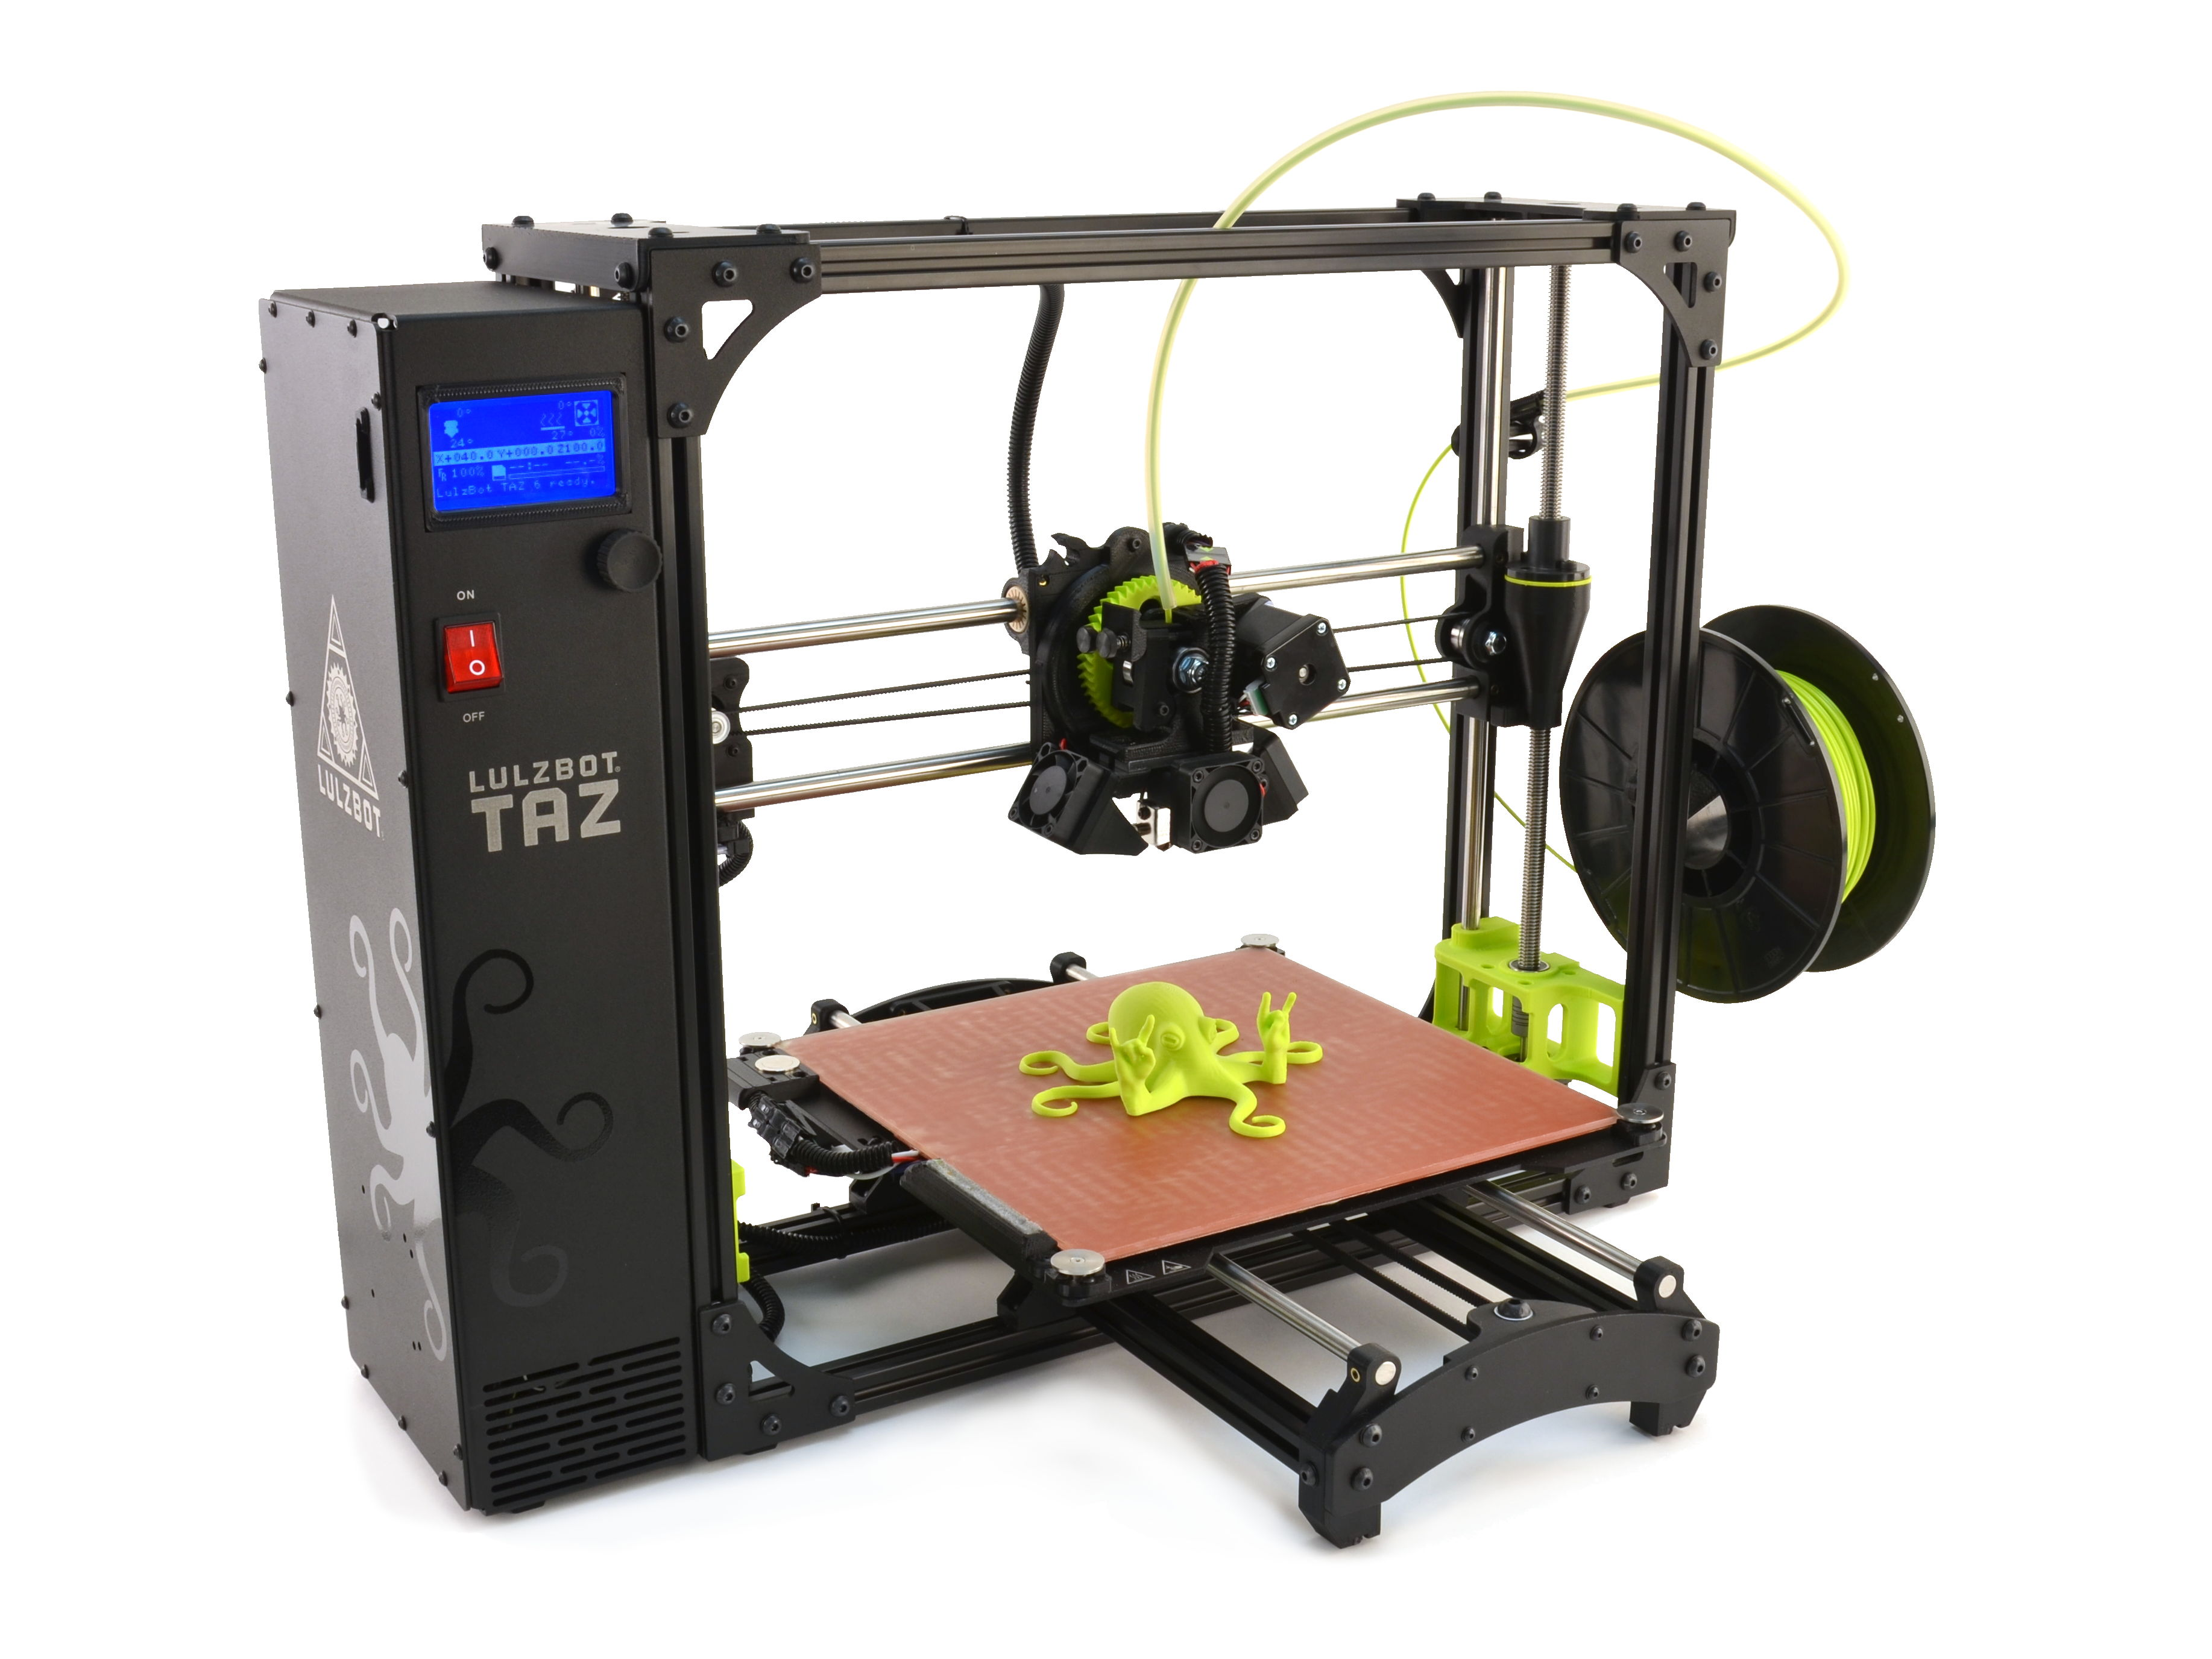
\includegraphics[keepaspectratio=true,angle=0,height=1.0\textheight,width=1.0\textwidth]{TAZ_6_Angle.JPG}

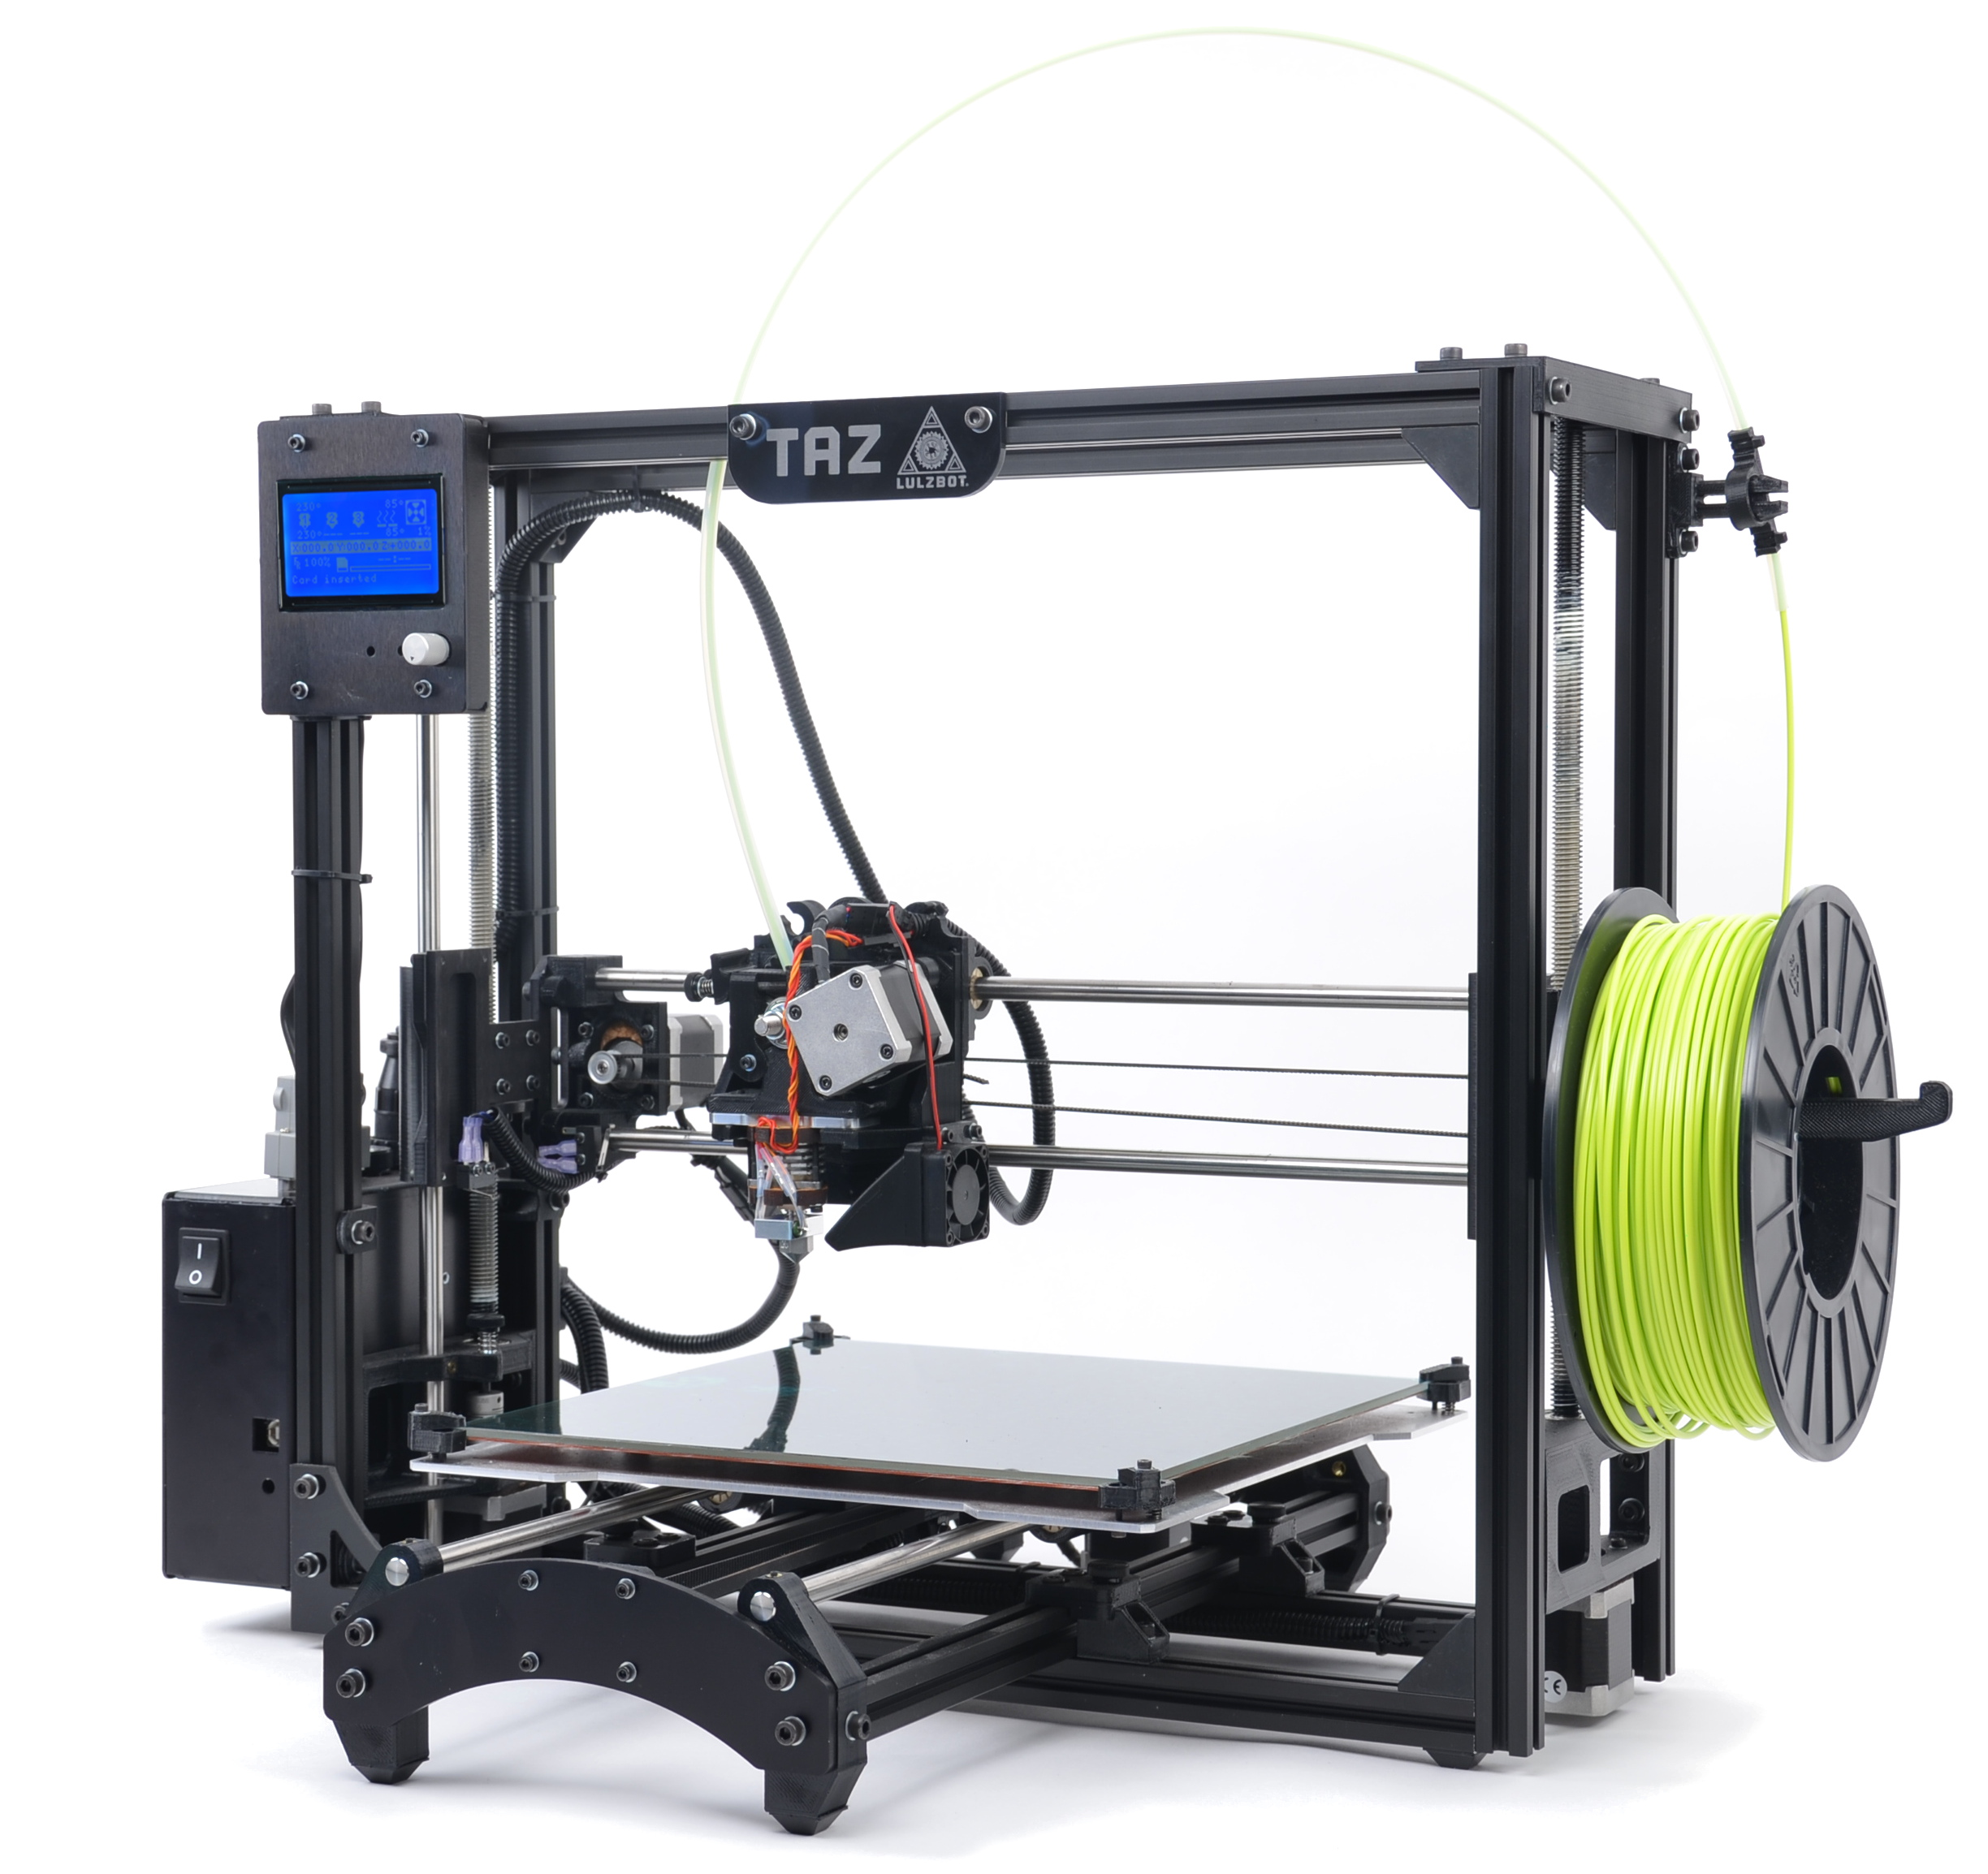
\includegraphics[keepaspectratio=true,angle=0,height=1.0\textheight,width=1.0\textwidth]{taz.jpg}


%\null\vfill
%\rule{0.4\textwidth}{0.4pt}
%\par
\begin{center}

\includegraphics[keepaspectratio=true,angle=0,height=0.25\textheight,width=0.25\textwidth]{Lulzbot_Logo_R_CMYK.eps}

{\large \itshape Aleph Objects, Inc.}
\end{center}
\endgroup
%\vspace*{0.1\textheight} 
%\newpage
%\clearpage
}
\fi
%%% END TITLE PAGE

%%% COPYRIGHT PAGE %%%
\ifcopyright
{\clearpage\null\vfill
\begingroup 
%\vfill\null 
\thispagestyle{empty}
\footnotesize\raggedright
\setlength{\parskip}{0.5\baselineskip}

\textbf{LulzBot\textsuperscript{\miniscule{\texttrademark}} TAZ 2.0 User Manual}

by Aleph Objects, Inc.

Copyright \copyright\ \the\year\ Aleph Objects, Inc.\par
Permission is granted to copy, distribute and\slash or modify 
this document under the terms of the
Creative Commons Attribution-ShareAlike 3.0 Unported license
(CC BY-SA 3.0).

Published by Aleph Objects, Inc., 123 SW 12th Street, Loveland, Colorado, 80537 USA.

For more information, call +1-970-377-1111 or go to \texttt{www.LulzBot.com} and \texttt{www.AlephObjects.com}.

ISBN: 978-0-9893784-2-0
\hfill\texttt{\the\year\the\month\the\day}
\endgroup
\pagebreak{}
}
\fi
%%% END COPYRIGHT PAGE %%%


%%% TABLE OF CONTENTS ToC %%%
\maxtocdepth{section}
% Dots
% space between dots
\renewcommand{\cftchapterdotsep}{15}
% dot symbol (default is period)
\renewcommand{\cftdot}{\textperiodcentered}	% centered period
% Set space between each entry in ToC
\setlength{\cftbeforechapterskip}{5pt}  % 5pt % 3pt
\tableofcontents*
%%% END TABLE OF CONTENTS ToC %%%

%%% LIST OF FIGURES %%%
%\addtodef{\listoffigures}{\clearpage\pagestyle{lof}}{}
% Fit all of List of Figures on one page
\renewcommand*{\lofheadstart}{\vspace{1cm}}
\clearpage
\listoffigures*
%%% END LIST OF FIGURES %%%

%%% CHAPTER STYLE %%%
\chapterstyle{jebinski} % defined in preamble
\def\topblockvspace{0.11}


%%% WARNINGS %%%
\ifwarnings
\chapter{\emph{WARNINGS}\protect \\
{Safety Information}}
\thispagestyle{empty}
\markboth{WARNING!}{Be Safe!}
{%
% Warnings.tex
%
% LulzBot® TAZ User Manual
%
% Copyright (C) 2014 Aleph Objects, Inc.
%
% This document is licensed under the Creative Commons Attribution 4.0
% International Public License (CC BY-SA 4.0) by Aleph Objects, Inc.
%

\section{\texttt{Read Me First!}}
\index{warnings}
\index{hazards}
\textcolor{red}{READ THIS MANUAL COMPLETELY BEFORE UNPACKING AND POWERING UP YOUR PRINTER.}

\section{\texttt{Hazards and Warnings}}

Your LulzBot\textsuperscript{\miniscule{\textregistered}} TAZ 3D printer has motorized and heated parts.  Always be aware of possible hazards when the printer is operational.


\subsection{\textcolor{red}{Electric Shock Hazard}}
\index{electronics}
\index{wires}
\index{power supply}
Never open the electronics case when the printer is powered on. Before removing the electronics case cover always power down the printer and completely turn off and unplug the power supply. Allow the power supply to discharge for at least one minute.

\subsection{\textcolor{red}{Burn Hazard}}
\index{extruder}
\index{heater block}
\index{temperature}
\index{burns}
Never touch the extruder nozzle or heater block without first turning off the hot end and allowing it to completely cool down. The hot end can take up to 20 minutes to completely cool. Never touch recently extruded plastic. The plastic can stick to your skin and cause burns. The heated bed can reach high temperatures that are capable of causing burns.

\subsection{\textcolor{red}{Fire Hazard}}
Never place flammable materials or liquids on or near the printer when it is powered on or operational. Liquid acetone and vapors are extremely flammable.

\subsection{\textcolor{red}{Pinch Hazard}}

When the printer is operational take care to never put your fingers in any moving parts including belts, pulleys, or gears. Tie back long hair or clothing that can get caught in the moving parts of the printer.

\subsection{\textcolor{red}{Static Charge}}
\index{static}
Make sure to ground yourself before touching the printer, especially its electronics. Electrostatic discharge can damage electronic components. Ground yourself by touching a grounded source like your computer case.

\subsection{\textcolor{red}{Age Warning}}

For users under the age of 18, adult supervision is recommended. Beware of choking hazards around small children.

\subsection{\textcolor{red}{Modifications and Repairs Warning}}

At Aleph Objects, Inc.\textsuperscript{\miniscule{\textregistered}} we respect your freedom to modify your LulzBot\textsuperscript{\miniscule{\textregistered}} desktop 3D printer. However any modifications or attempted repairs that cause damage are not covered under the Warranty. Questions? Contact Technical Support by emailing support@lulzbot.com, or by calling +1-970-377-1111.

\subsection{\texttt{Federal Communications Commission Statement}}
\index{FCC}
Note: This equipment has been tested and found to comply with the limits for a Class A digital device, pursuant to part 15 of the FCC Rules. These limits are designed to provide reasonable protection against harmful interference when the equipment is operated in a commercial environment. This equipment generates, uses, and can radiate radio frequency energy and, if not installed and used in accordance with the instruction manual, may cause harmful interference to radio communications. Operation of this equipment in a residential area is likely to cause harmful interference in which case the user will be required to correct the interference at his own expense.

This device complies with part 15 class A of the FCC Rules. Operation is subject to the following two conditions:
\begin{enumerate}
\item This device may not cause harmful interference and
\item This device must accept any interference received, including interference that may cause undesired operation.
\end{enumerate}

\textcolor{red}{FCC Warning:}
\textcolor{red}{Changes or modifications not approved by the party responsible for compliance could void the users authority to operate the equipment.}



}
\fi
%%% END WARNINGS %%%

%%% END FRONTMATTER %%%
%%% BEGIN MAINMATTER %%%
\mainmatter*

% Set page numbering to arabic, but don't reset numbering (*)
\pagenumbering*{arabic}

%%% UNPACKING %%%
\ifunpacking
\chapter{\emph{Unpacking Your Printer}}
\thispagestyle{empty}
\markboth{Unpacking Your Printer}{LulzBot\textsuperscript{\miniscule{\texttrademark}} TAZ User Manual}
{\index{instructions}

\begin{figure}[hbt]
\centering
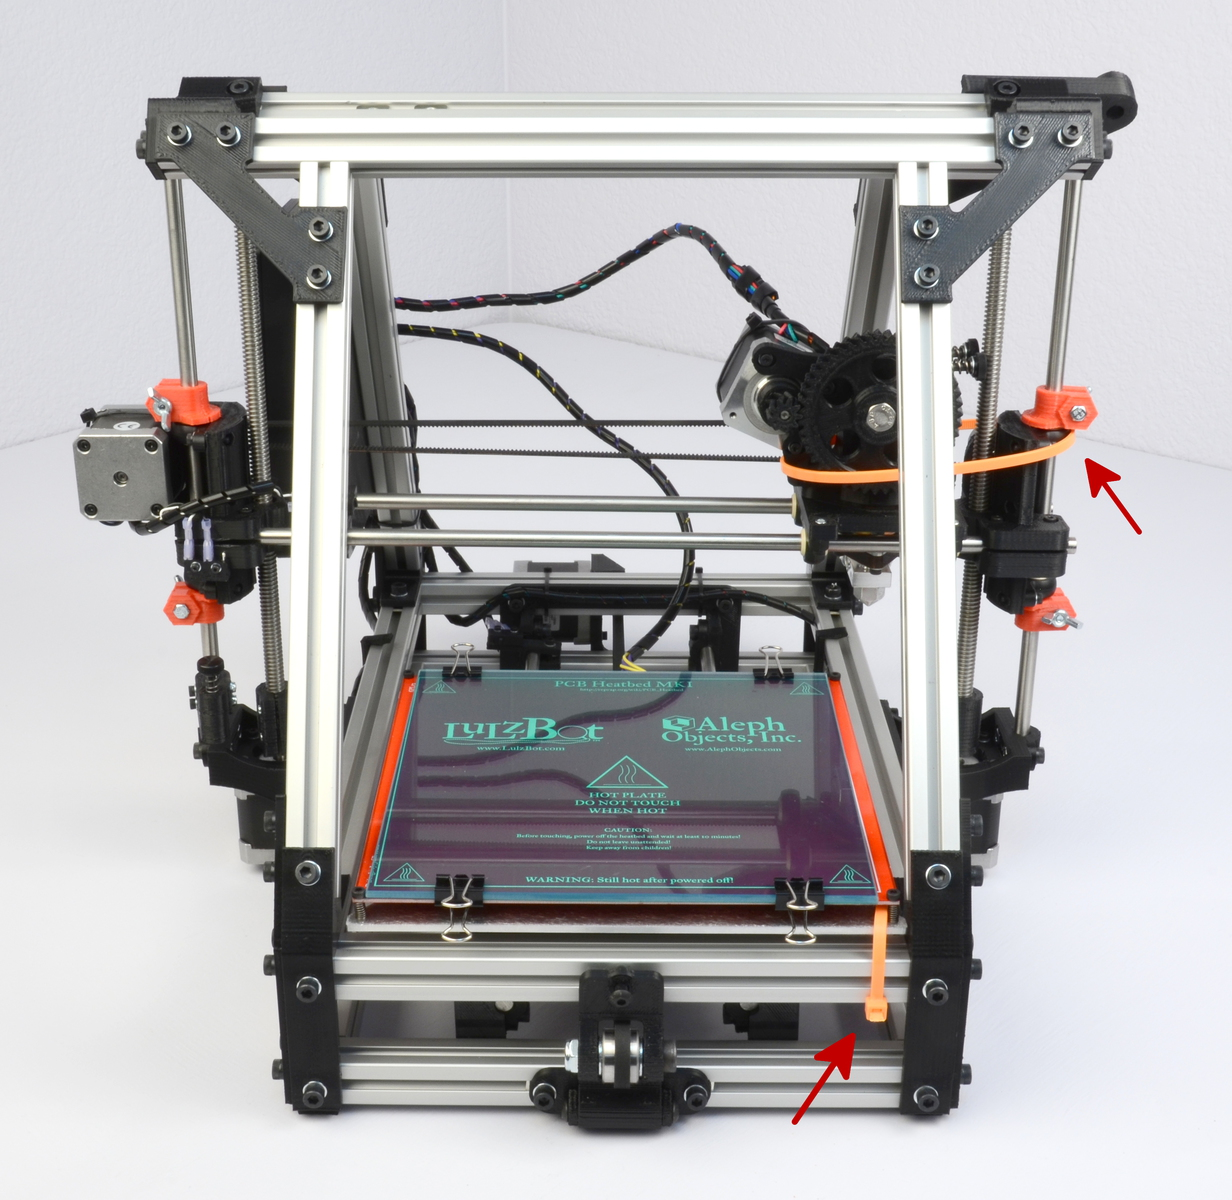
\includegraphics[keepaspectratio=true,angle=0,height=0.4\textheight,width=1.0\textwidth]{zip_ties.jpg}
\caption{Orange Zip Ties}
\label{fig:zip_ties}
\end{figure}

\begin{enumerate}
\item Remove the plastic bag containing instructions, cords, and small parts.

\index{foam padding}
\item Remove the top foam padding. 

\index{filament spool}
\index{filament guide}
\item Slowly remove the two smaller foam pads. One of these pads will contain the plastic filament spool and plastic filament guide. The other pad will contain the 5lb coil of ABS plastic filament. With the two small foam pads remove and set aside these items.

\index{power supply}
\index{tool bag}
\item Remove the white power supply box and the black tool bag. These items are along opposite sides of the printer.

\item Grab the top of the wrapped printer on the top center where you will feel two lengths of square aluminum tubing. Holding the top two tubes, SLOWLY pull the printer upwards out of the box. The two large side foam pads should fall off when the printer is out of the box.

\item Set you printer on a stable level surface.

\item Gently unwrap the pink ESD plastic covering the printer. Remove the rolled sheet of PET tape from below the print bed. Gently lift the printer to slide the plastic wrapping from under the printer. 

\item Find the item list attached to the plastic bag of parts. Before you move on to setting up your printer make sure all of the items on the list are in your package.

\item Using scissors or wire cutters, cut and remove the two ORANGE plastic zip ties
(Fig. \ref{fig:zip_ties}, page \pageref{fig:zip_ties})
. One zip tie is located on the bottom front of the printer on the print bed. The other zip tie is wrapped around the extruder carriage and X axis. Make sure to not cut any of the surrounding wires or belts.

\begin{figure}[hbt]
\centering
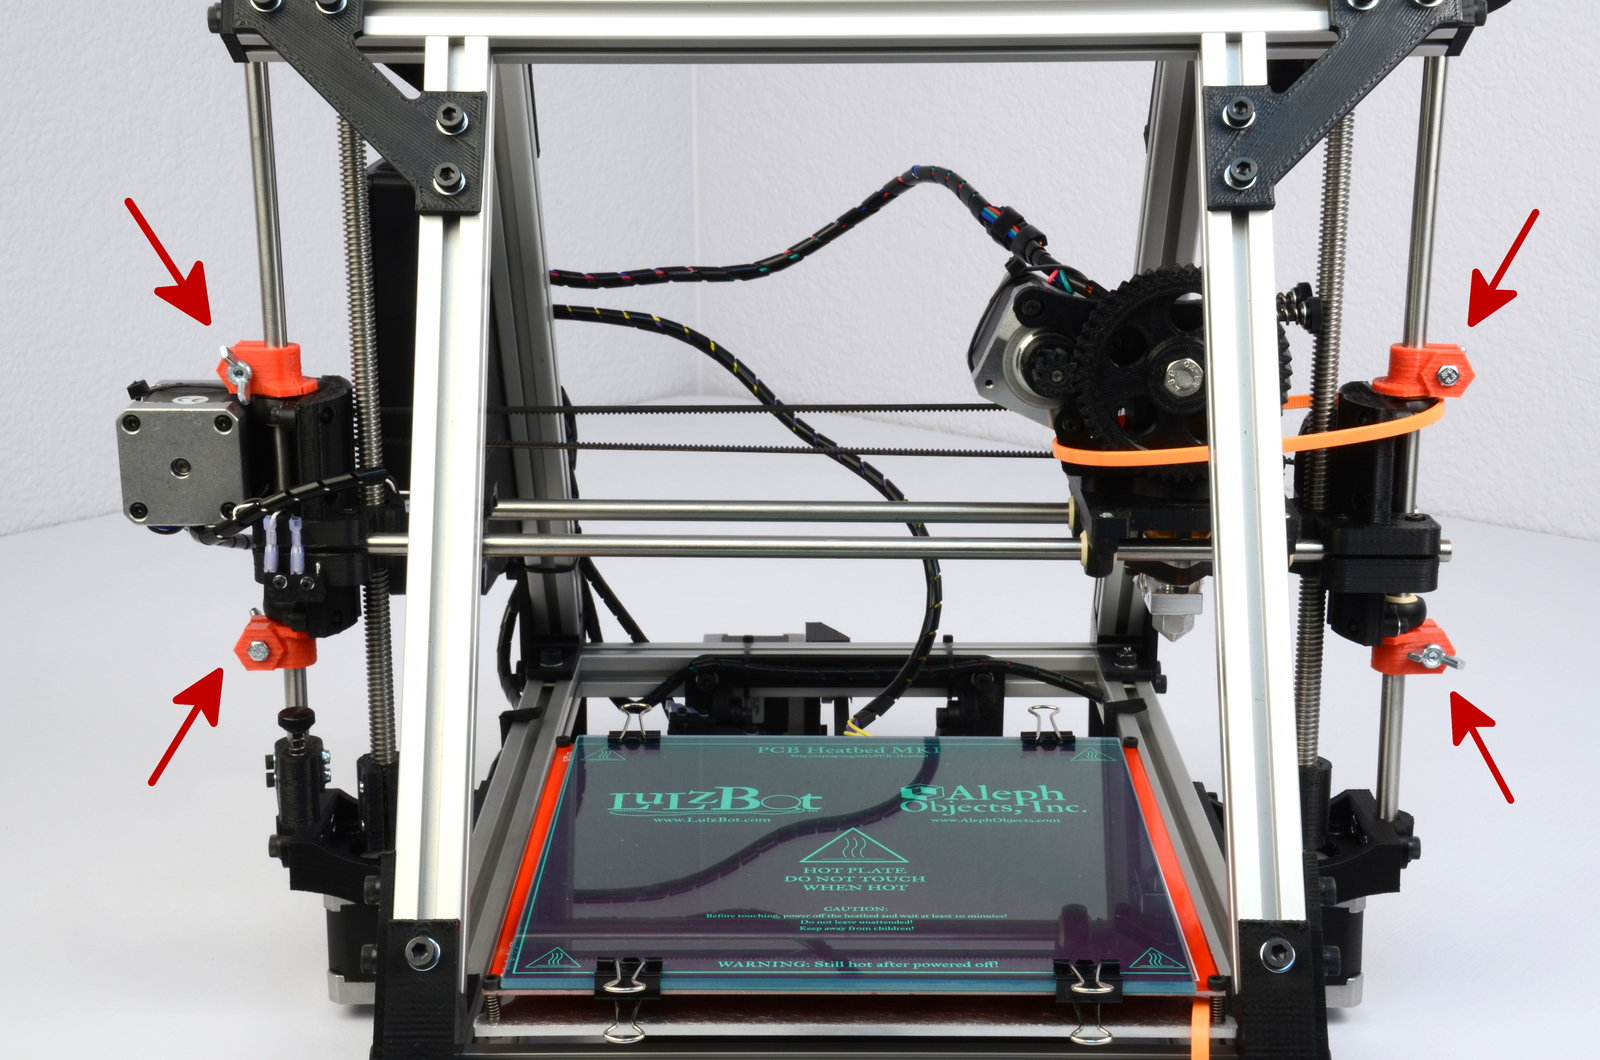
\includegraphics[keepaspectratio=true,angle=0,height=0.4\textheight,width=1.0\textwidth]{shipping_clamps.jpg}
\caption{Red Shipping Clamps}
\label{fig:shipping_clamps}
\end{figure}

\index{shipping clamps}
\index{x-end motor mount}
\index{idler}
\item Remove the four red shipping clamps above and below the x-end motor mount and idler
(Fig. \ref{fig:shipping_clamps}, page \pageref{fig:shipping_clamps}).

\item Loosen and remove the wing nut and screw on each of the four clamps. Remove each of the four clamps by popping them off of the smooth rod. Use a screwdriver or wrench to pry open and remove the clamps if you have trouble removing them by hand (Fig. \ref{fig:shipping_clamps_pry}, page \pageref{fig:shipping_clamps_pry}). Keep the clamps and hardware for future use if you need to ship or transport your printer.

\begin{figure}[hbt]
\centering
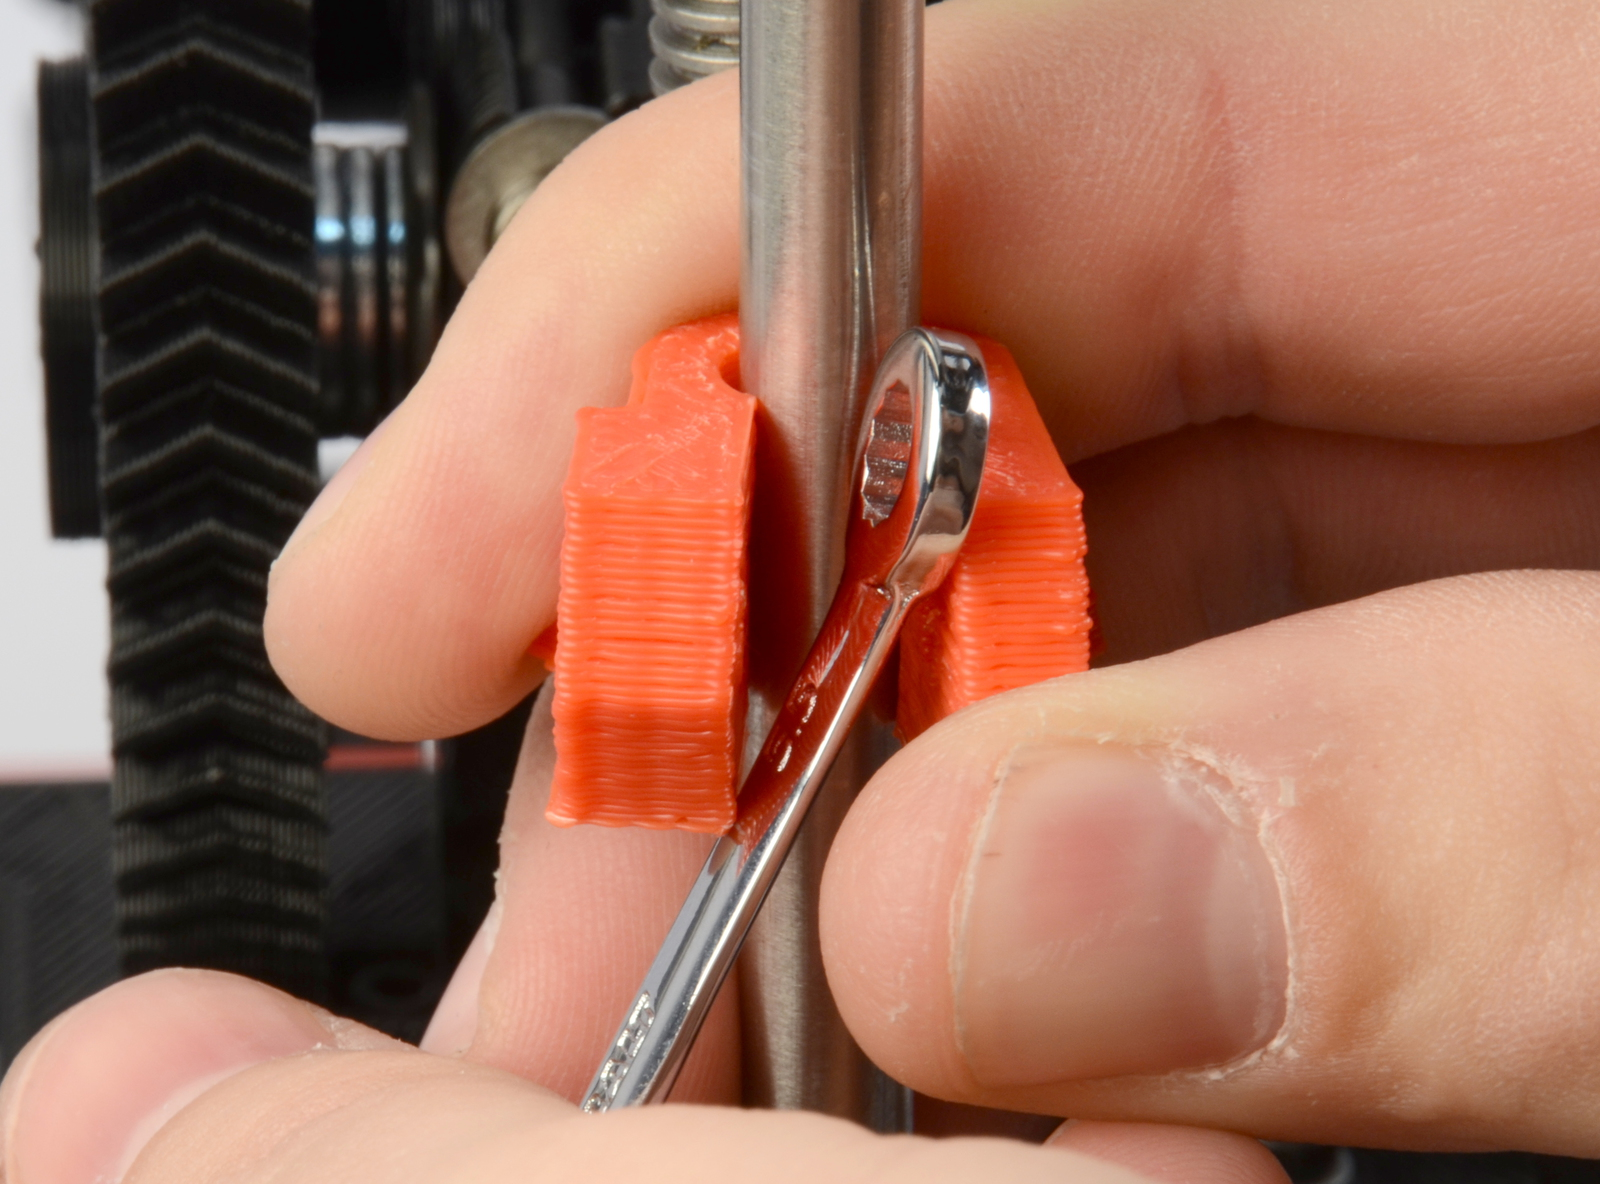
\includegraphics[keepaspectratio=true,angle=0,height=0.4\textheight,width=1.0\textwidth]{shipping_clamps_pry.jpg}
\caption{Using a wrench to pry off the shipping clamps}
\label{fig:shipping_clamps_pry}
\end{figure}

\index{blue tape}
\index{PET sheet}
\item Remove the blue tape from the sides of the print surface. Make sure to not remove the green PET tape on the glass print surface. The PET tape helps keep the print attached to the print surface during printing.

\end{enumerate}
}
\fi
%%% END UNPACKING %%%

%%% SETUP %%%
\ifsetup
\chapter{\emph{Setup Your Printer}}
\thispagestyle{empty}
\markboth{Setup Your Printer}{LulzBot\textsuperscript{\miniscule{\texttrademark}} TAZ User Manual}
{\begin{enumerate}
\item Your printer has been pre-calibrated and tested; however, after unpacking all of the components you will need to re-mount the Y axis onto the frame and connect the bed and Y axis connectors. You will also need to re-mount the extruder toolhead. Please follow the steps completely to make certain that the extruder toolhead and Y axis are re-mounted correctly and you will be on your way to your first print.

\item Place the TAZ frame and Y axis assembly on a flat and level surface. Move to the Y axis assembly and find the four Y axis bolts. The four bolts, located on the Y axis aluminum frame bars, have large plastic knobs that allow the bolts to be easily turned by hand (Fig. \ref{fig:Y_axis_bolts}, page \pageref{fig:Y_axis_bolts}). Turning counter clock-wise, remove each of the four Y axis bolts and set aside (Fig. \ref{fig:remove_Y_axis_bolts}, page \pageref{fig:remove_Y_axis_bolts}).

\begin{figure}[hp]
\centering
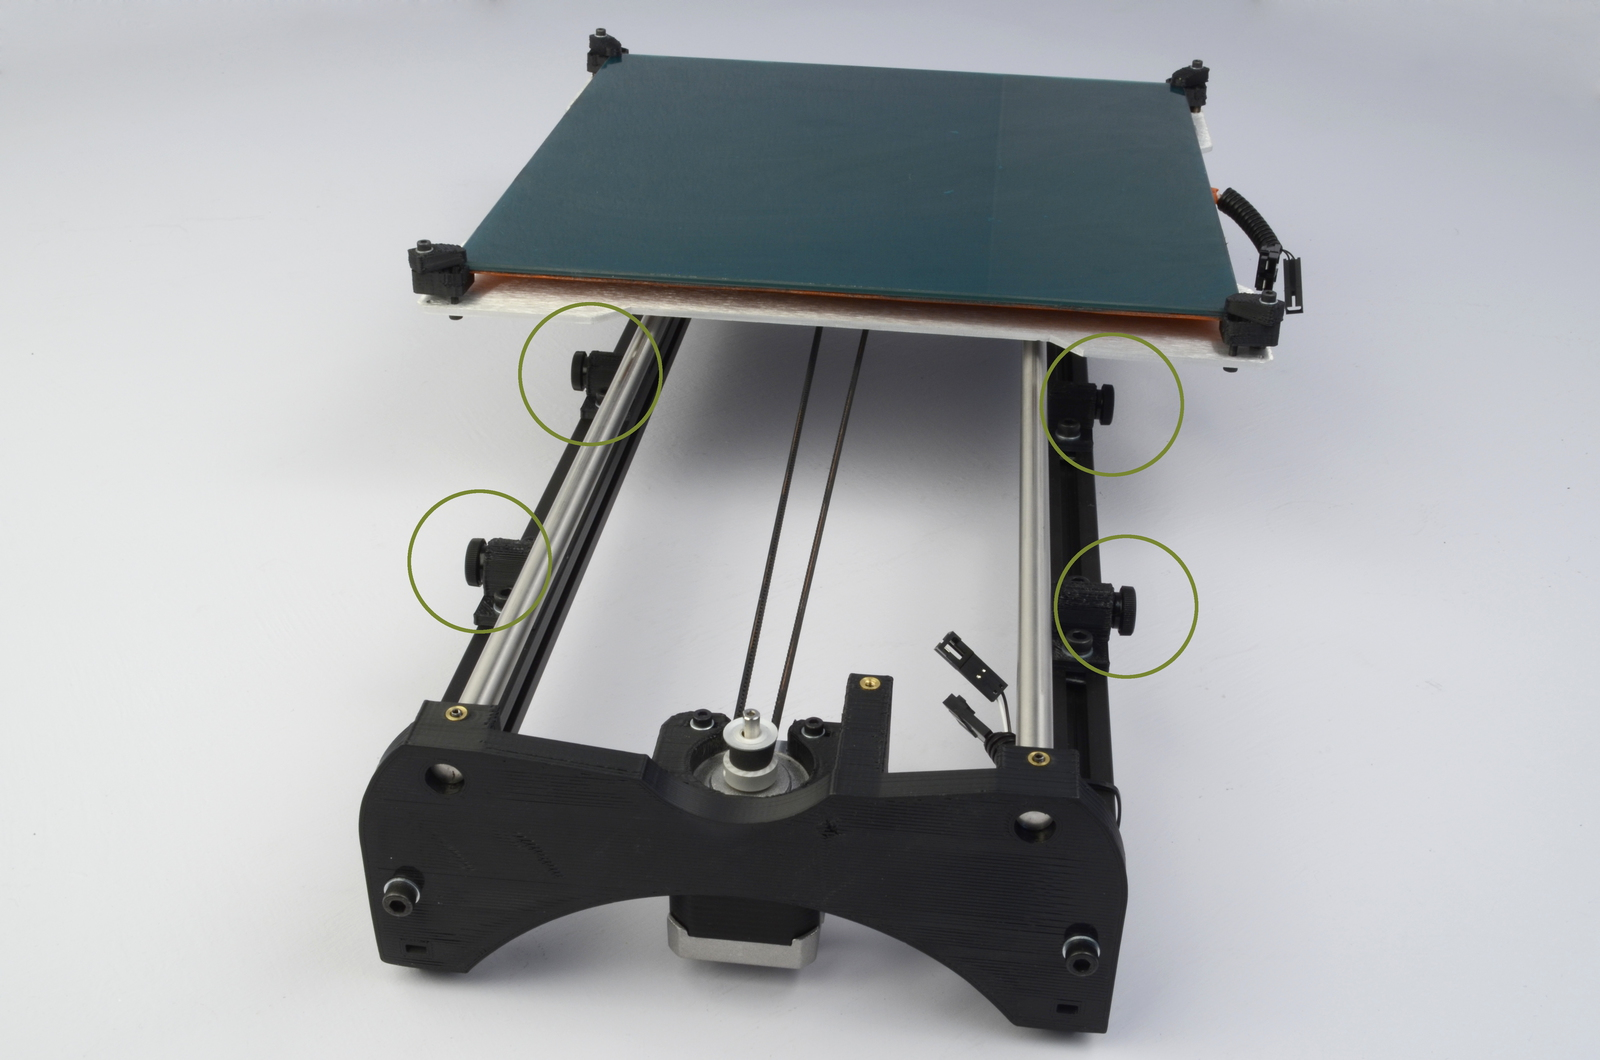
\includegraphics[keepaspectratio=true,angle=0,height=0.4\textheight,width=1.0\textwidth]{y_axis_bolts.JPG}
\caption{Locate the four Y axis bolts}
\label{fig:Y_axis_bolts}
\end{figure}

%\begin{figure}[hp] CD changed to force pic placement
\begin{figure}[H]
\centering
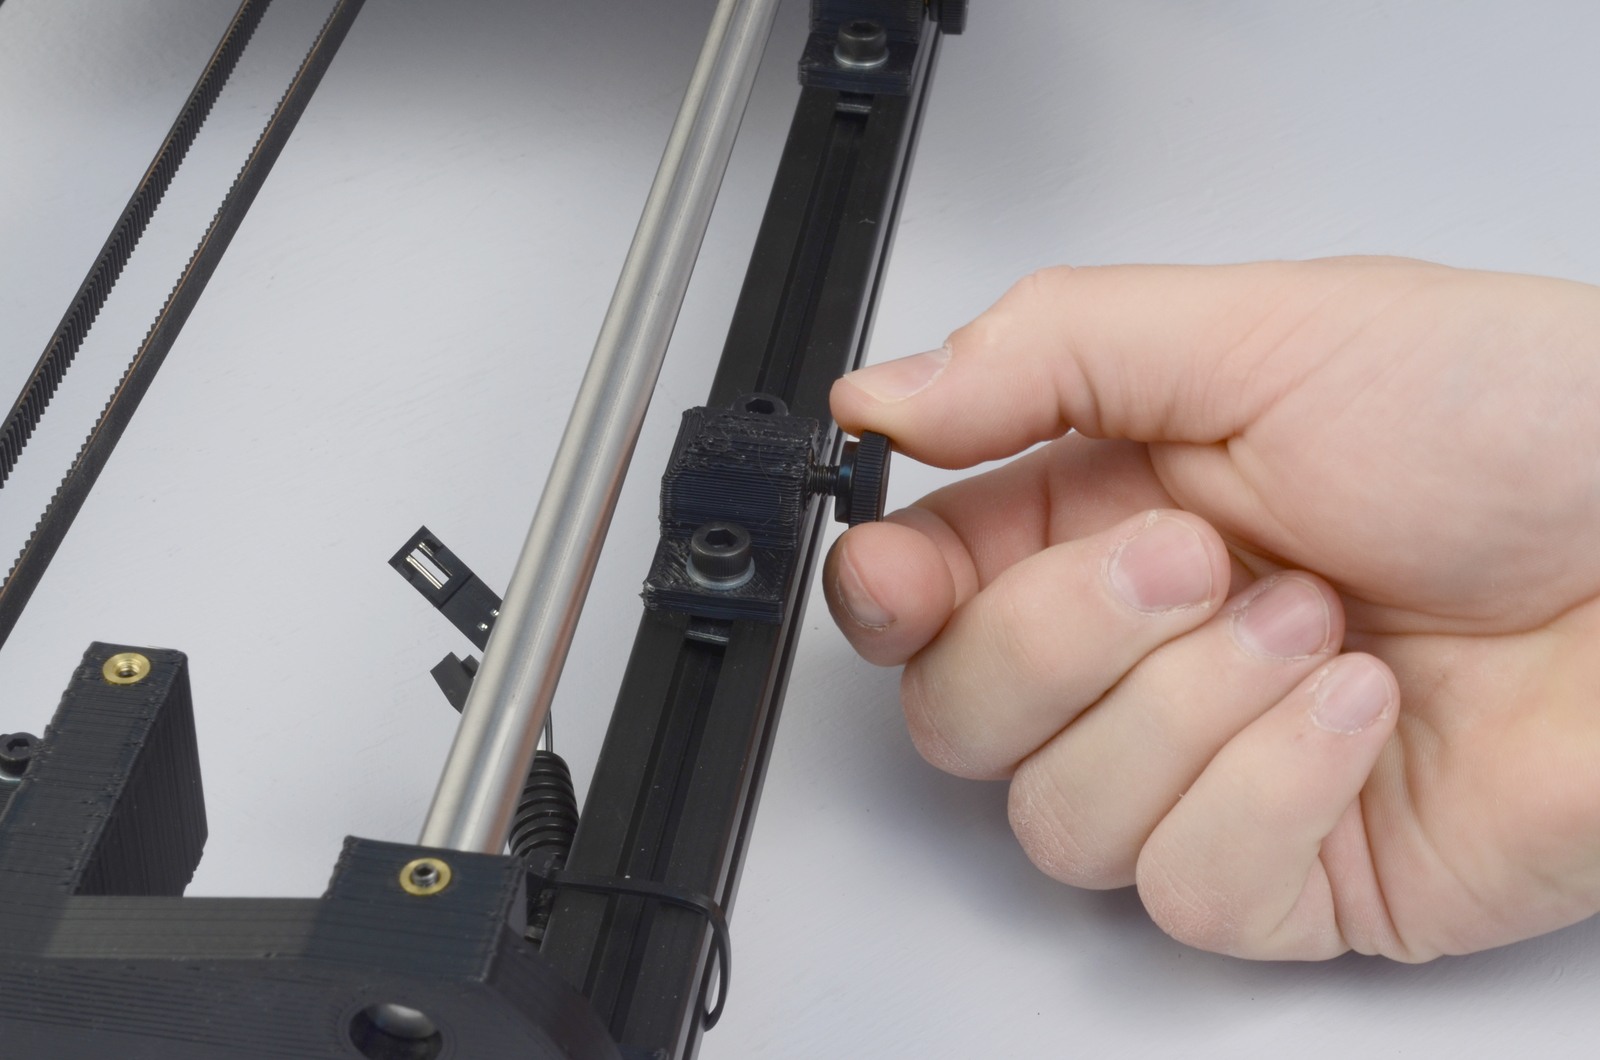
\includegraphics[keepaspectratio=true,angle=0,height=0.4\textheight,width=1.0\textwidth]{y_axis_bolt_remove.JPG}
\caption{Remove the four Y axis bolts}
\label{fig:remove_Y_axis_bolts}
\end{figure}

\item On the TAZ frame locate the four Y axis mount brackets shown in Fig. \ref{fig:frame_Y_axis_mounts} (pg. \pageref{fig:frame_Y_axis_mounts}). With the print surface facing up and the stepper motor end of the Y axis facing back, slide the Y axis assembly in between the Y axis mount brackets. The four Y axis mount brackets will line up with the Y axis bolt holes on the Y axis assembly. Thread the four Y axis bolts through the brackets, into the Y axis assembly (Fig. \ref{fig:Y_axis_bolts_tighten}, page \pageref{fig:Y_axis_bolts_tighten}). Before completely tightening the Y axis bolts make sure the Y axis aluminum bars are pushed down against the TAZ frame lower bars. You can do this by slightly tilting the printer, on the side edge, enough to lift the feet of the Y axis off of the table. The weight of the Y axis will seat it against the TAZ frame. While the printer is slightly tilted tighten the four Y axis bolts. The printer can be now be set flat on the table.
%\begin{figure}[hp] CD forcing image placement
\begin{figure}[H]
\centering
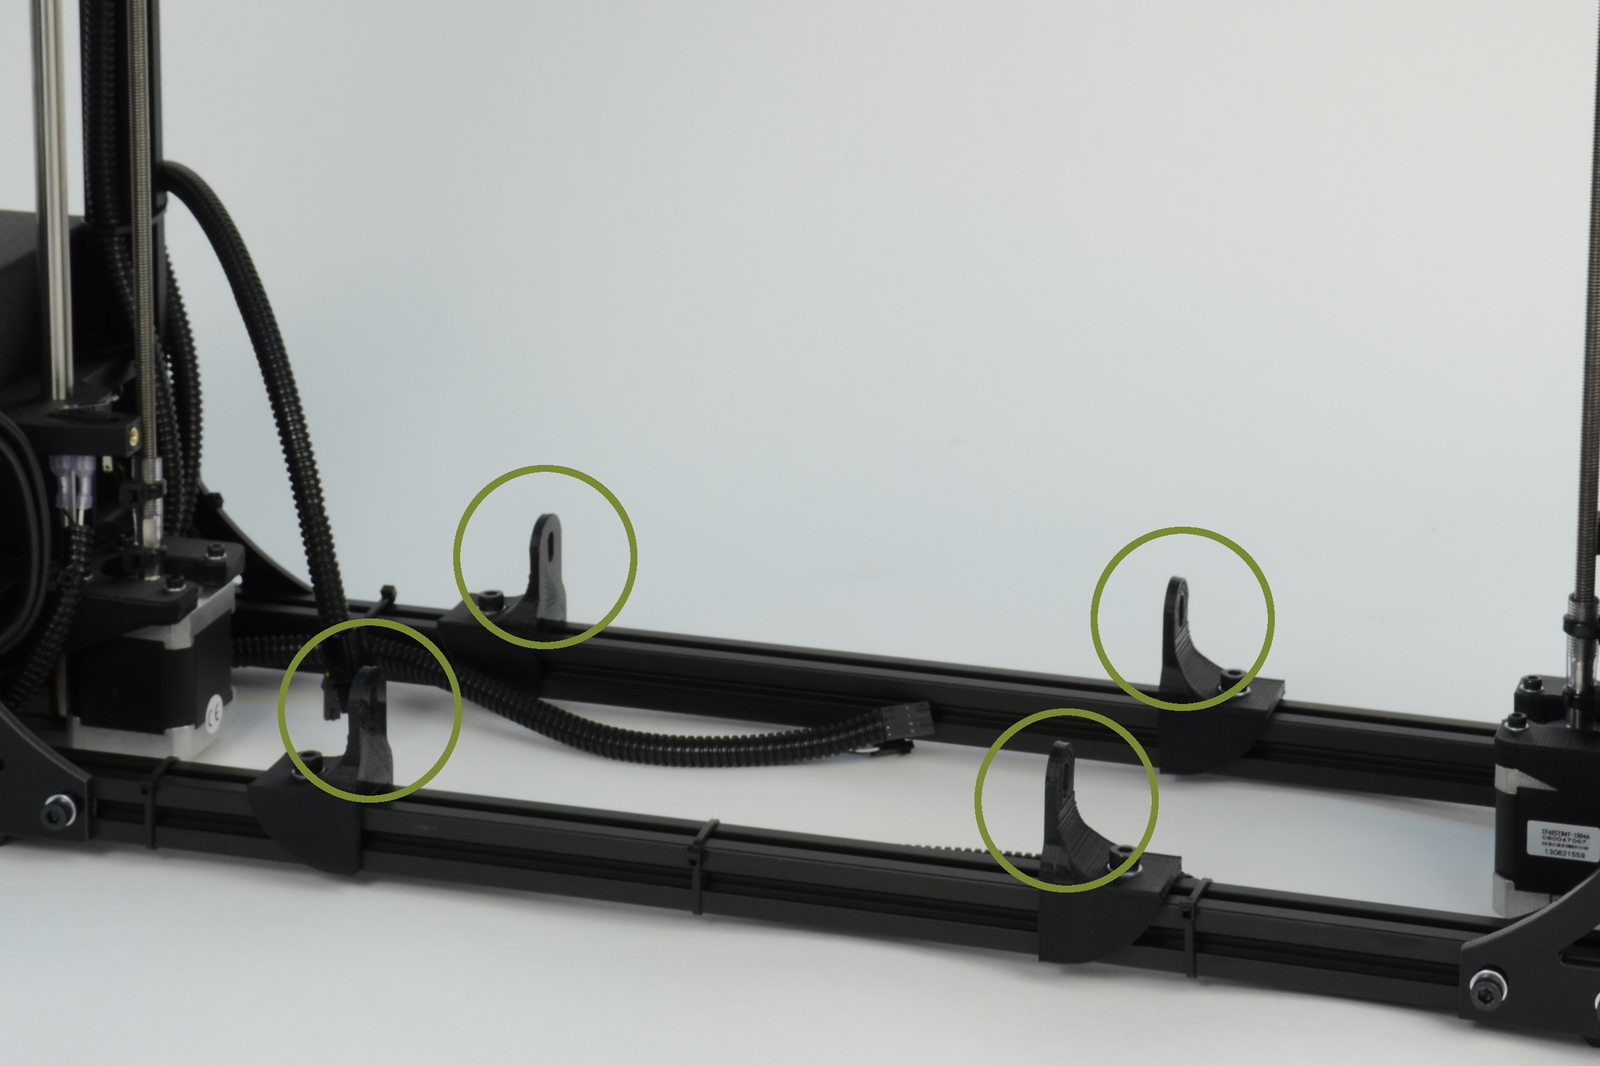
\includegraphics[keepaspectratio=true,angle=0,height=0.4\textheight,width=1.0\textwidth]{frame_y_axis_connector.JPG}
\caption{Locate the four Y axis mounts on the frame}
\label{fig:frame_Y_axis_mounts}
\end{figure}

%\begin{figure}[hp] CD forcing image placement
\begin{figure}[H]
\centering
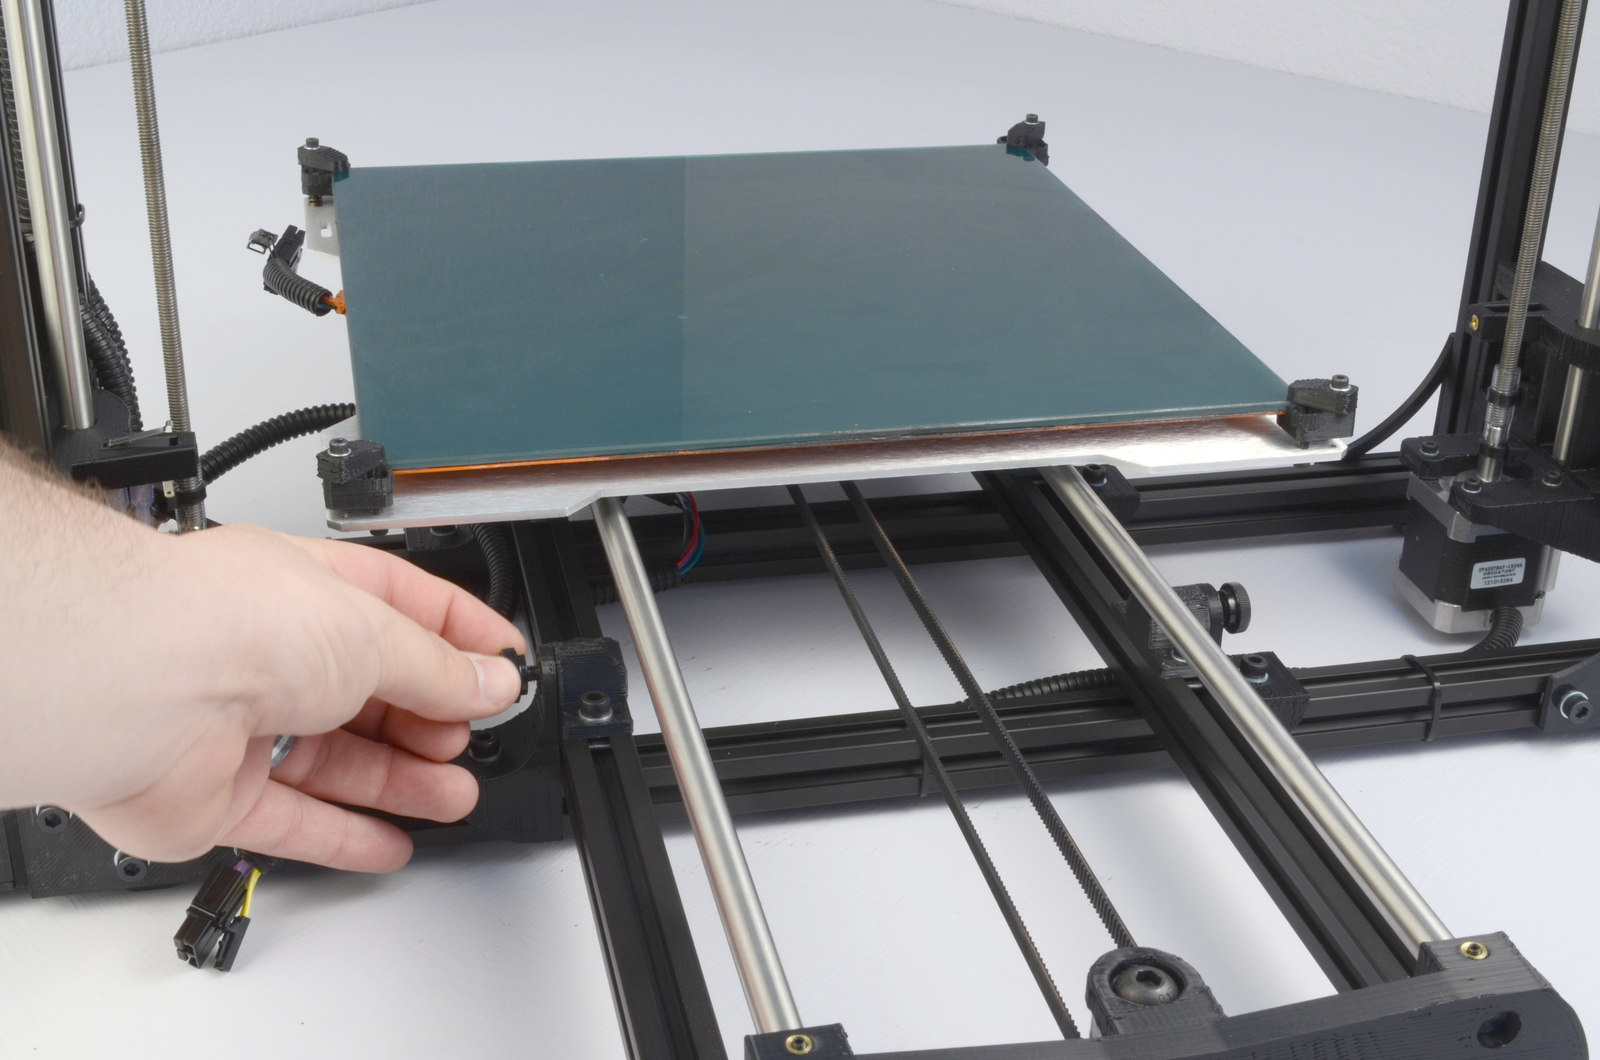
\includegraphics[keepaspectratio=true,angle=0,height=0.4\textheight,width=1.0\textwidth]{y_axis_bolt_tighten.JPG}
\caption{Screw in and tighten the four Y axis bolts}
\label{fig:Y_axis_bolts_tighten}
\end{figure}

\item The final step of installing the Y axis is connecting the print surface connectors and Y axis connectors. Pull the print bed completely to the front of the printer to get access to the Y axis connectors. You will find matching male and female 4 pin stepper motor connectors and two pin end stop connectors. Connect the matching male and female connectors (Fig. \ref{fig:Y_axis_connectors}, page \pageref{fig:Y_axis_connectors}); make sure the connector lock clicks to be sure that the connection is secure.


\begin{figure}[p]
\centering
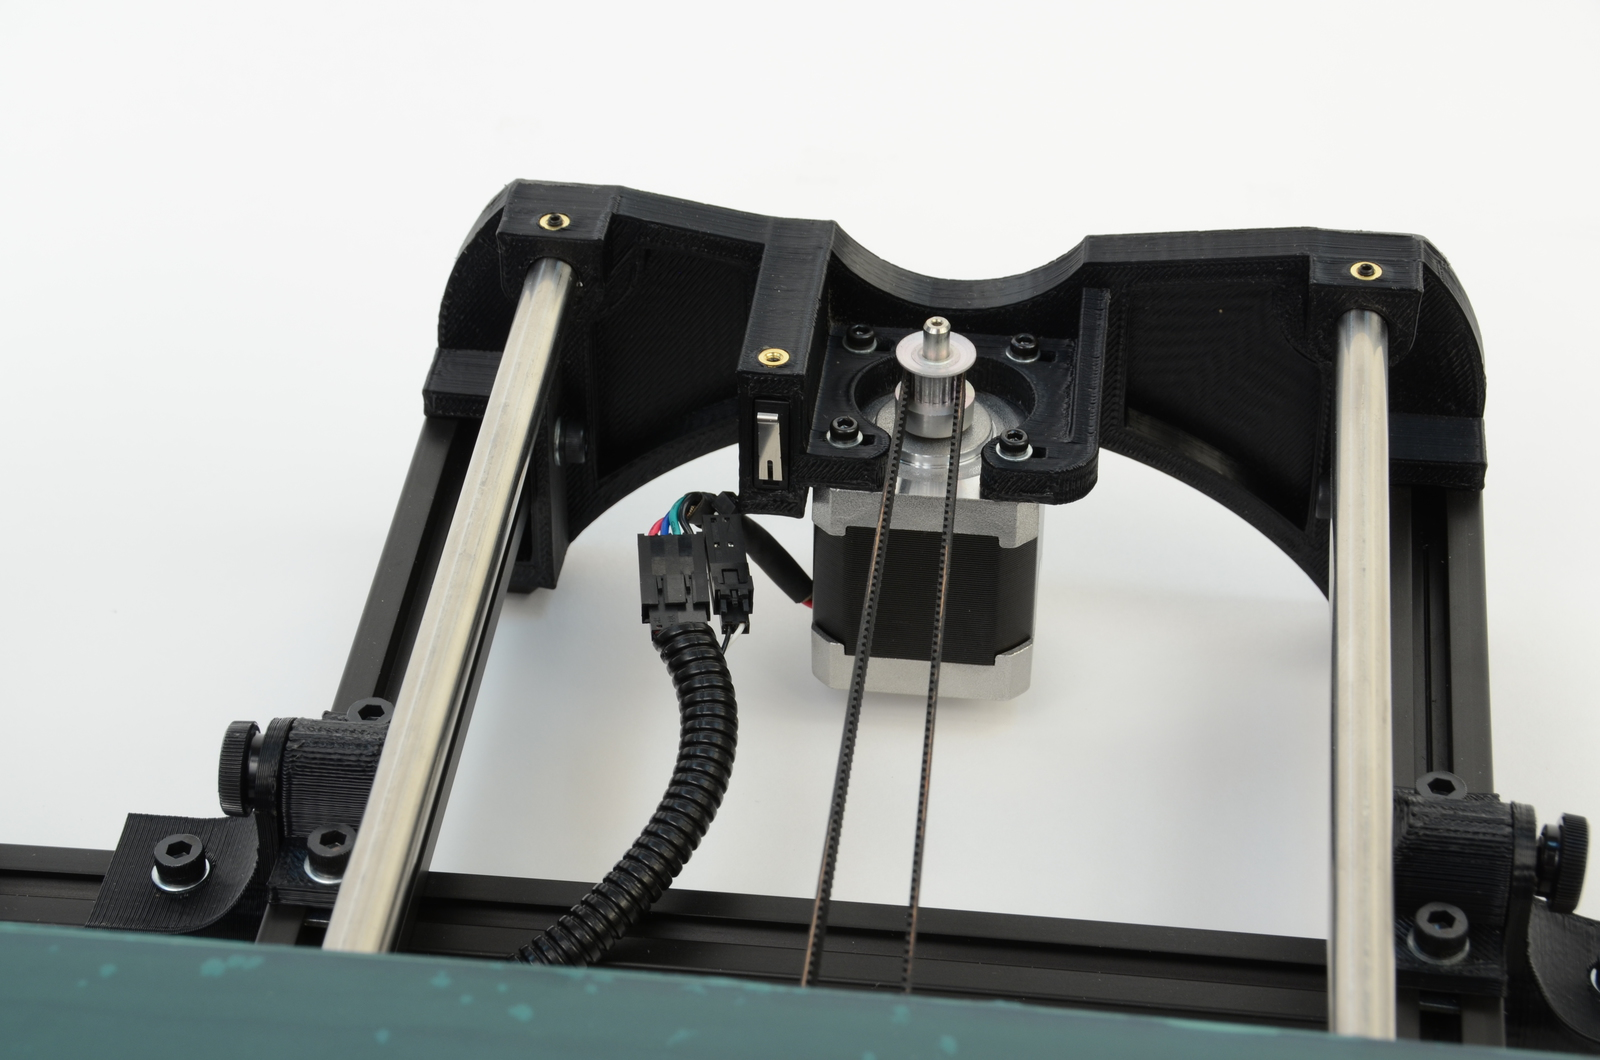
\includegraphics[keepaspectratio=true,angle=0,height=0.4\textheight,width=1.0\textwidth]{y_axis_connectors.JPG}
\caption{Connect the two connectors found at the rear of the Y axis}
\label{fig:Y_axis_connectors}
\end{figure}

\item Locate the two connectors to the left of the print bed. Connect the matching female and male large two pin heat bed connectors and the small two pin connectors (Fig. \ref{fig:bed_connectors}, page \pageref{fig:bed_connectors}).

\begin{figure}[p]
\centering
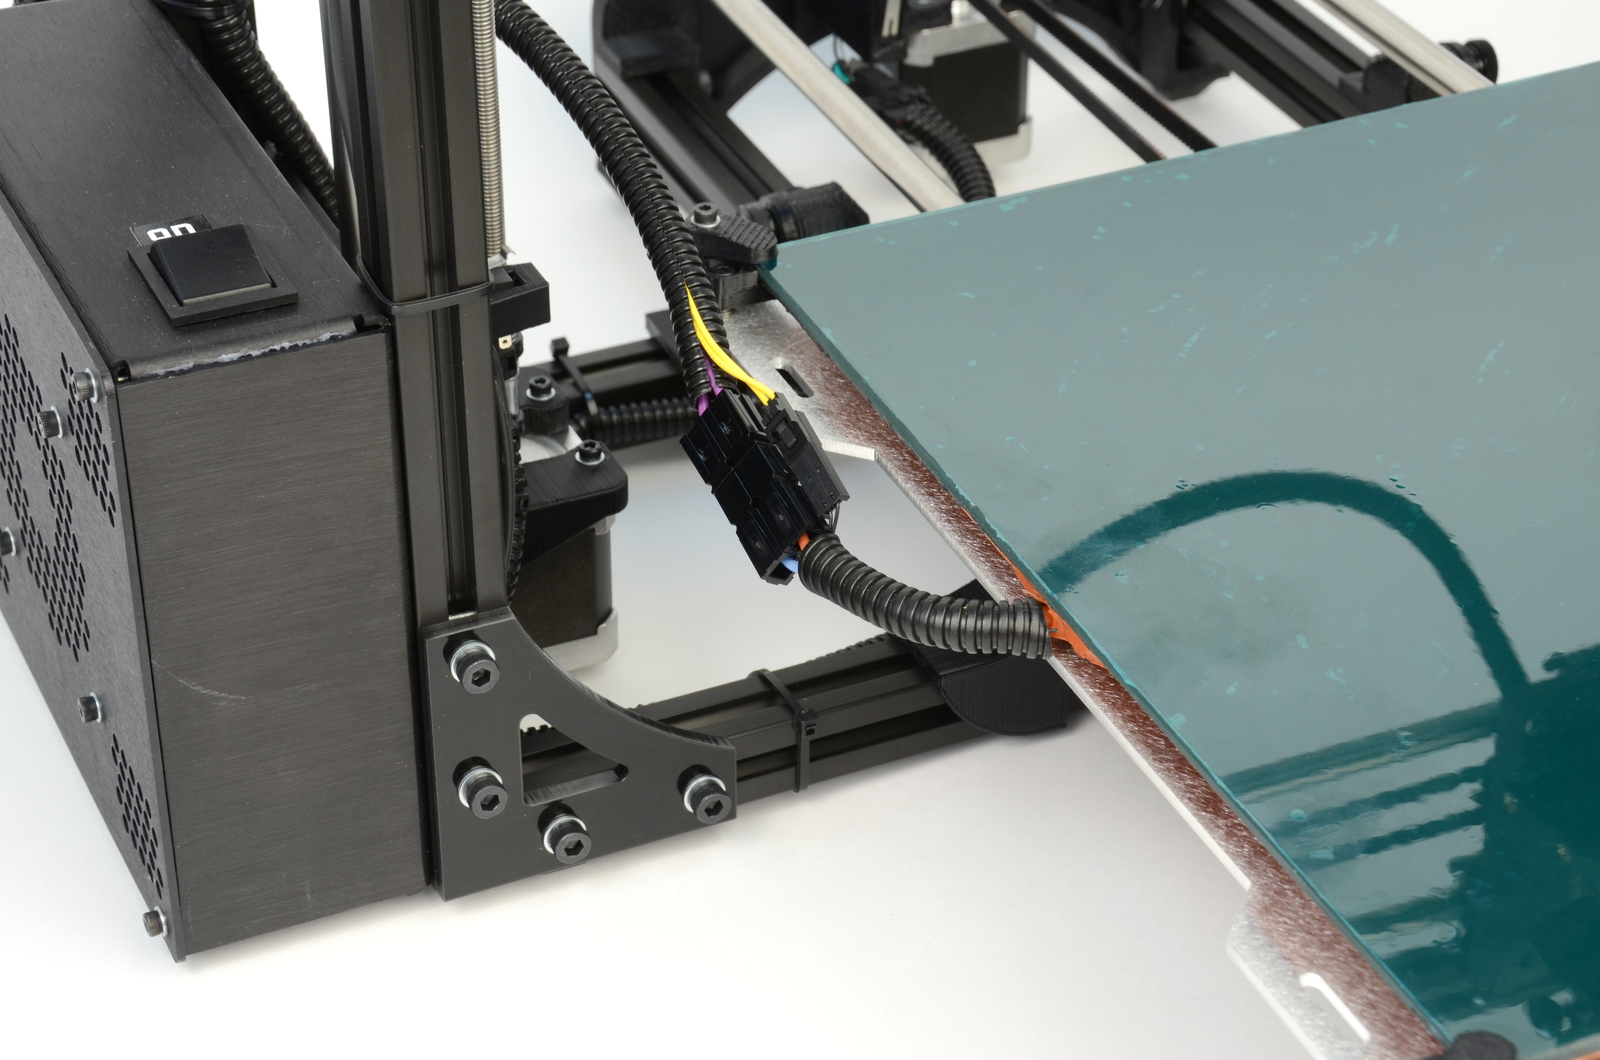
\includegraphics[keepaspectratio=true,angle=0,height=0.4\textheight,width=1.0\textwidth]{bed_connectors.JPG}
\caption{Connect the two connectors on the left of the print bed}
\label{fig:bed_connectors}
\end{figure}

\item Locate the two small black zip ties that are included in the documents bag (Fig. \ref{fig:bed_connectors_strain_relief}, page \pageref{fig:bed_connectors_strain_relief}). Wrap the two zip ties through the slot, located on the left rear of the aluminum bed plate, and around the print bed wires (Fig. \ref{fig:bed_connectors_strain_relief_done}, page \pageref{fig:bed_connectors_strain_relief_done}). Tighten the zip ties snug so the wire cannot move freely. Cut off the excess end of the zip ties with the needle nose pliers included in the tool bag.

%\begin{figure}[hp] CD forcing image placement
\begin{figure}[H]
\centering
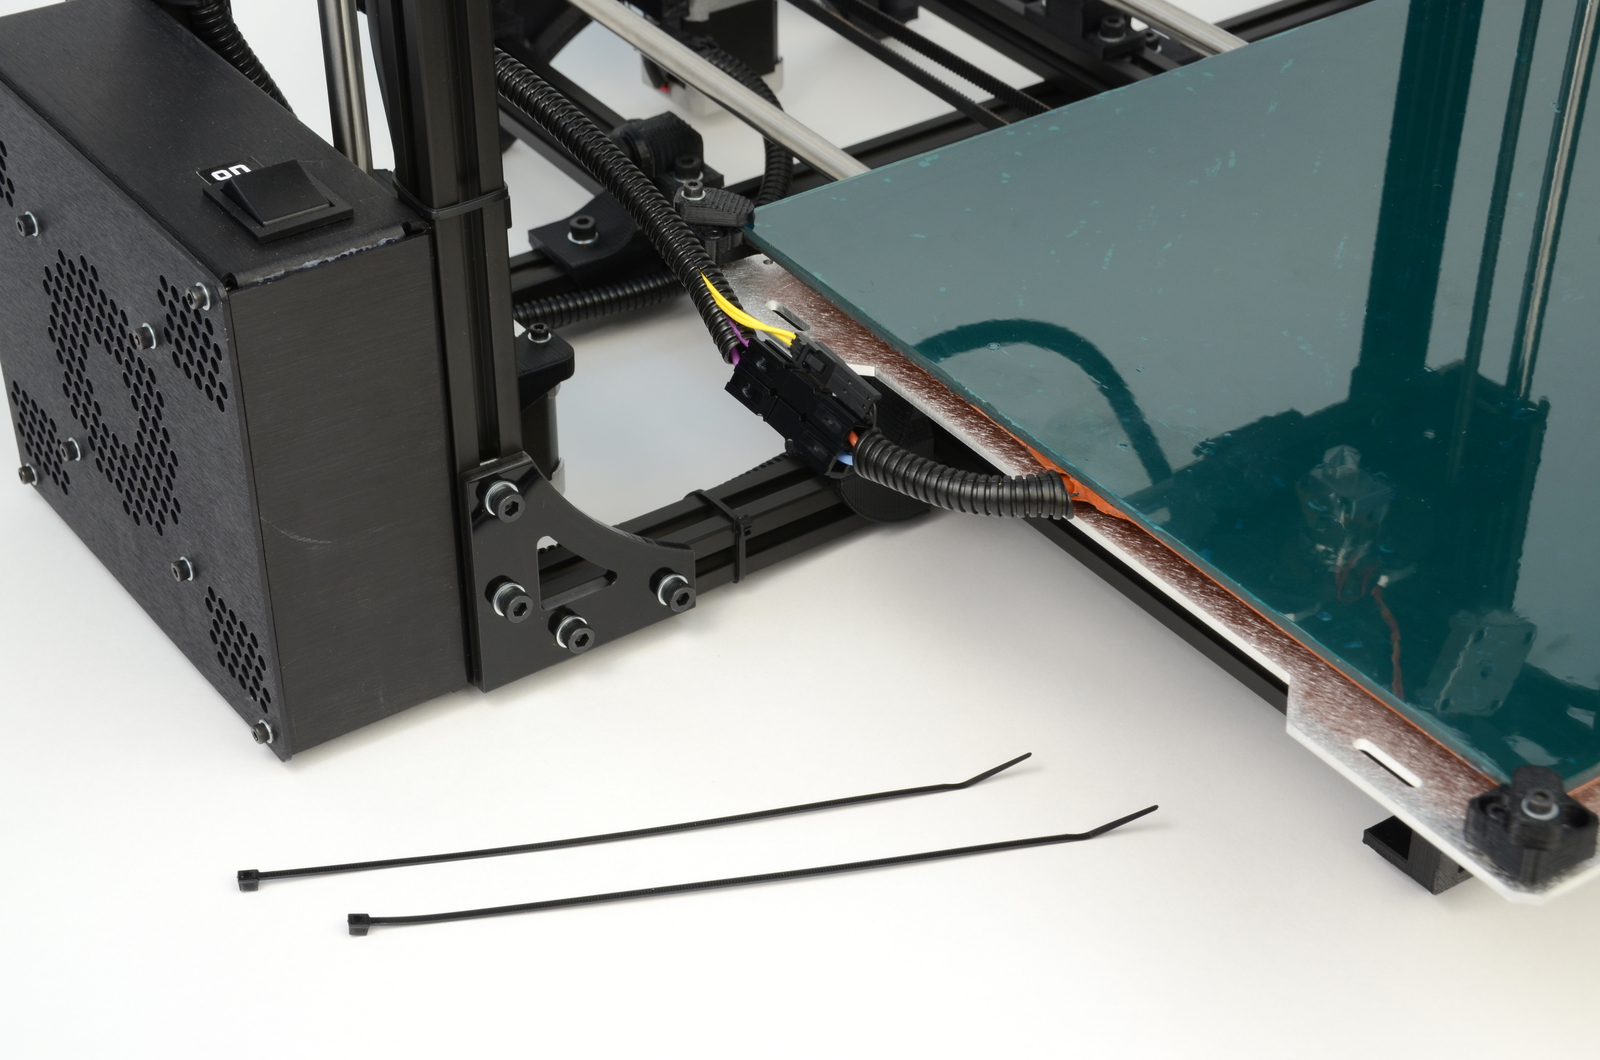
\includegraphics[keepaspectratio=true,angle=0,height=0.4\textheight,width=1.0\textwidth]{bed_connectors_strain_relief.JPG}
\caption{Locate the two zip ties found in the bag with the manual}
\label{fig:bed_connectors_strain_relief}
\end{figure}

%\begin{figure}[hp] CD forcing image placement
\begin{figure}[H]
\centering
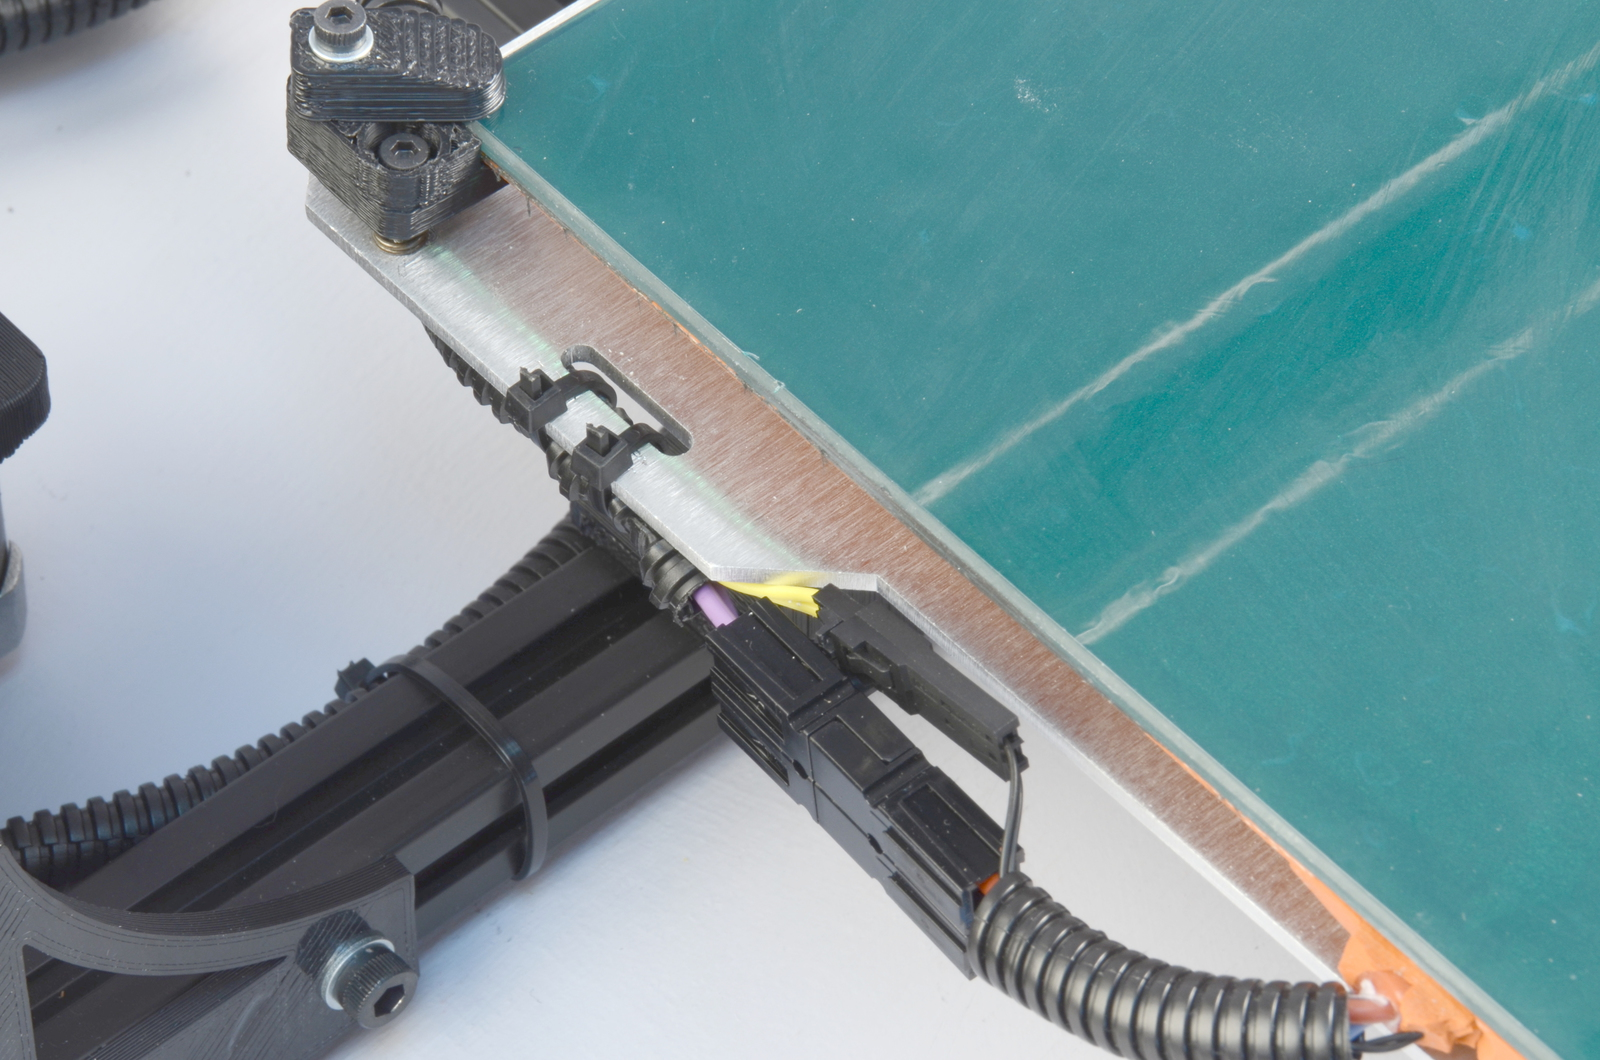
\includegraphics[keepaspectratio=true,angle=0,height=0.4\textheight,width=1.0\textwidth]{bed_connectors_strain_relief_done.JPG}
\caption{Tightly wrap the zip ties around the bed wires and through the strain relief slot}
\label{fig:bed_connectors_strain_relief_done}
\end{figure}

\item Move the X axis carriage over to the center of the smooth rods. Remove the foam from between the X axis carriage and the X axis ends. Locate the extruder toolhead screw from the accessories bag and place the extruder toolhead onto the X axis carriage. The extruder mount will slide into the bottom portion of the carriage and self center. Use the included 2.5mm driver to secure the extruder tool head onto the X axis carriage.
\begin{figure}[hp]
\centering
\includegraphics[keepaspectratio=true,angle=0,height=0.4\textheight,width=1.0\textwidth]{PIC_of_extruder mount installation.JPG}
\caption{Mount the extruder tool head}
\label{fig:PIC-of-initial-position}
\end{figure}

\item Connect the stepper motor and the hot end to the existing wiring harness. The connections are keyed and can only be connected in the correct orientation.
\begin{figure}[hp]
\centering
\includegraphics[keepaspectratio=true,angle=0,height=0.4\textheight,width=1.0\textwidth]{PIC_of_extruder_connections.JPG}
\caption{Extruder connections}
\label{fig:PIC_of_extruder_connections}
\end{figure}

\item Secure the wiring harness into the strain relief on the top left hand side of the X axis carriage. 
\begin{figure}[hp]
\centering
\includegraphics[keepaspectratio=true,angle=0,height=0.4\textheight,width=1.0\textwidth]{PIC_of_strain_relief.JPG}
\caption{Strain relief installation}
\label{fig:PIC_of_strain_relief}
\end{figure}

\item Now that the Y axis is mounted and the extruder tool head is installed you should set your printer on a stable, flat, and level surface large enough for extra space around the printer. Make sure your printer work space is clear of anything that could obstruct the movement of the printer. \textcolor{red}{Make sure there are no flammable fabrics or liquids near the printer space}. It is also best to not put your printer near a drafty window or air conditioner vent.

\index{power supply}
\index{USB cable}
\item Unwrap the power supply and USB cables.

\textcolor{red}{MAKE SURE THE POWER SUPPLY IS COMPLETELY UNPLUGGED BEFORE MOVING ON TO THE NEXT STEP}.

\index{electronics receptacles}
\item Locate the power supply and USB receptacles along the back of the TAZ electronics enclosure
(Fig. \ref{fig:electronics_plugs}, page \pageref{fig:electronics_plugs}). Locate the power supply and the included AC power cable (Fig. \ref{fig:power_supply}, page \pageref{fig:power_supply}). Locate the DC power cable plug on the power supply. Connect the DC locking plug into the DC connector on the TAZ electronics enclosure (Fig. \ref{fig:ps_plug}, page \pageref{fig:ps_plug}). The plug is keyed which may require rotating the plug until the keys line up and the plug can be pushed in. Once you have pushed in the plug turn the locking sleeve clockwise until it is tight against the electronics enclosure (Fig. \ref{fig:electronics_plugs_plugged-in}, page \pageref{fig:electronics_plugs_plugged-in}).
%\begin{figure}[hbt]
\begin{figure}[H]
\centering
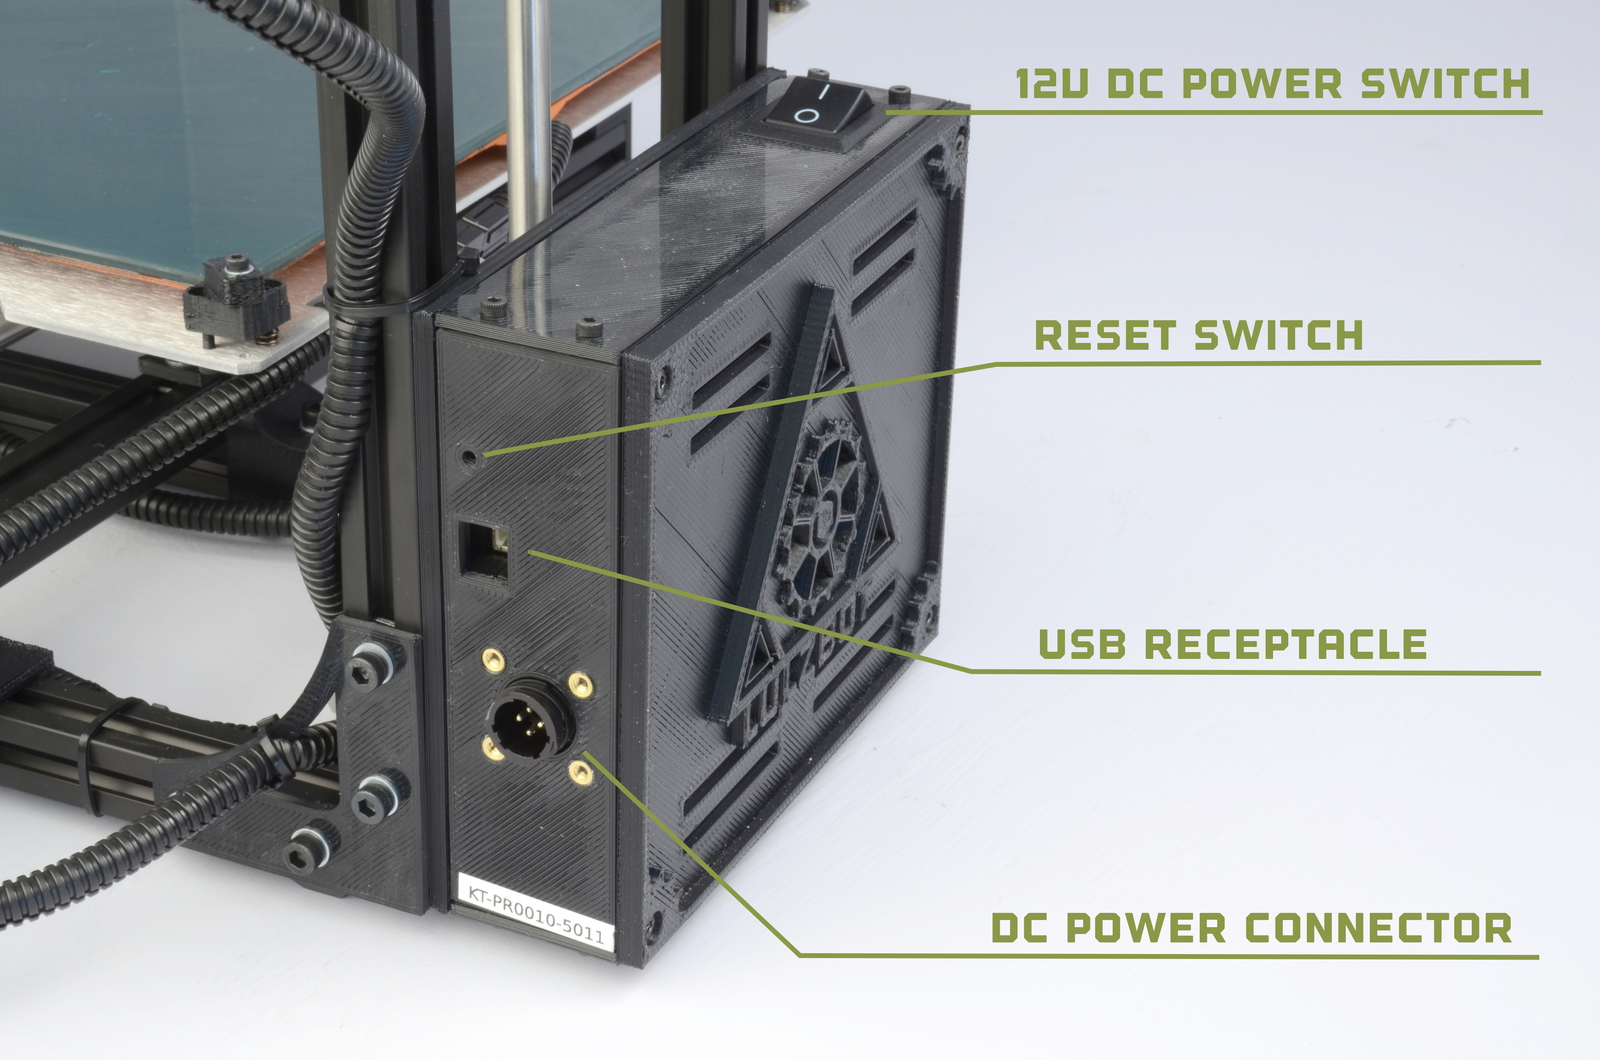
\includegraphics[keepaspectratio=true,angle=0,height=0.4\textheight,width=1.0\textwidth]{electronics_case_rec.JPG}
\caption{Power supply and USB receptacles}
\label{fig:electronics_plugs}
\end{figure}

%\begin{figure}[hp]
\begin{figure}[H]
\centering
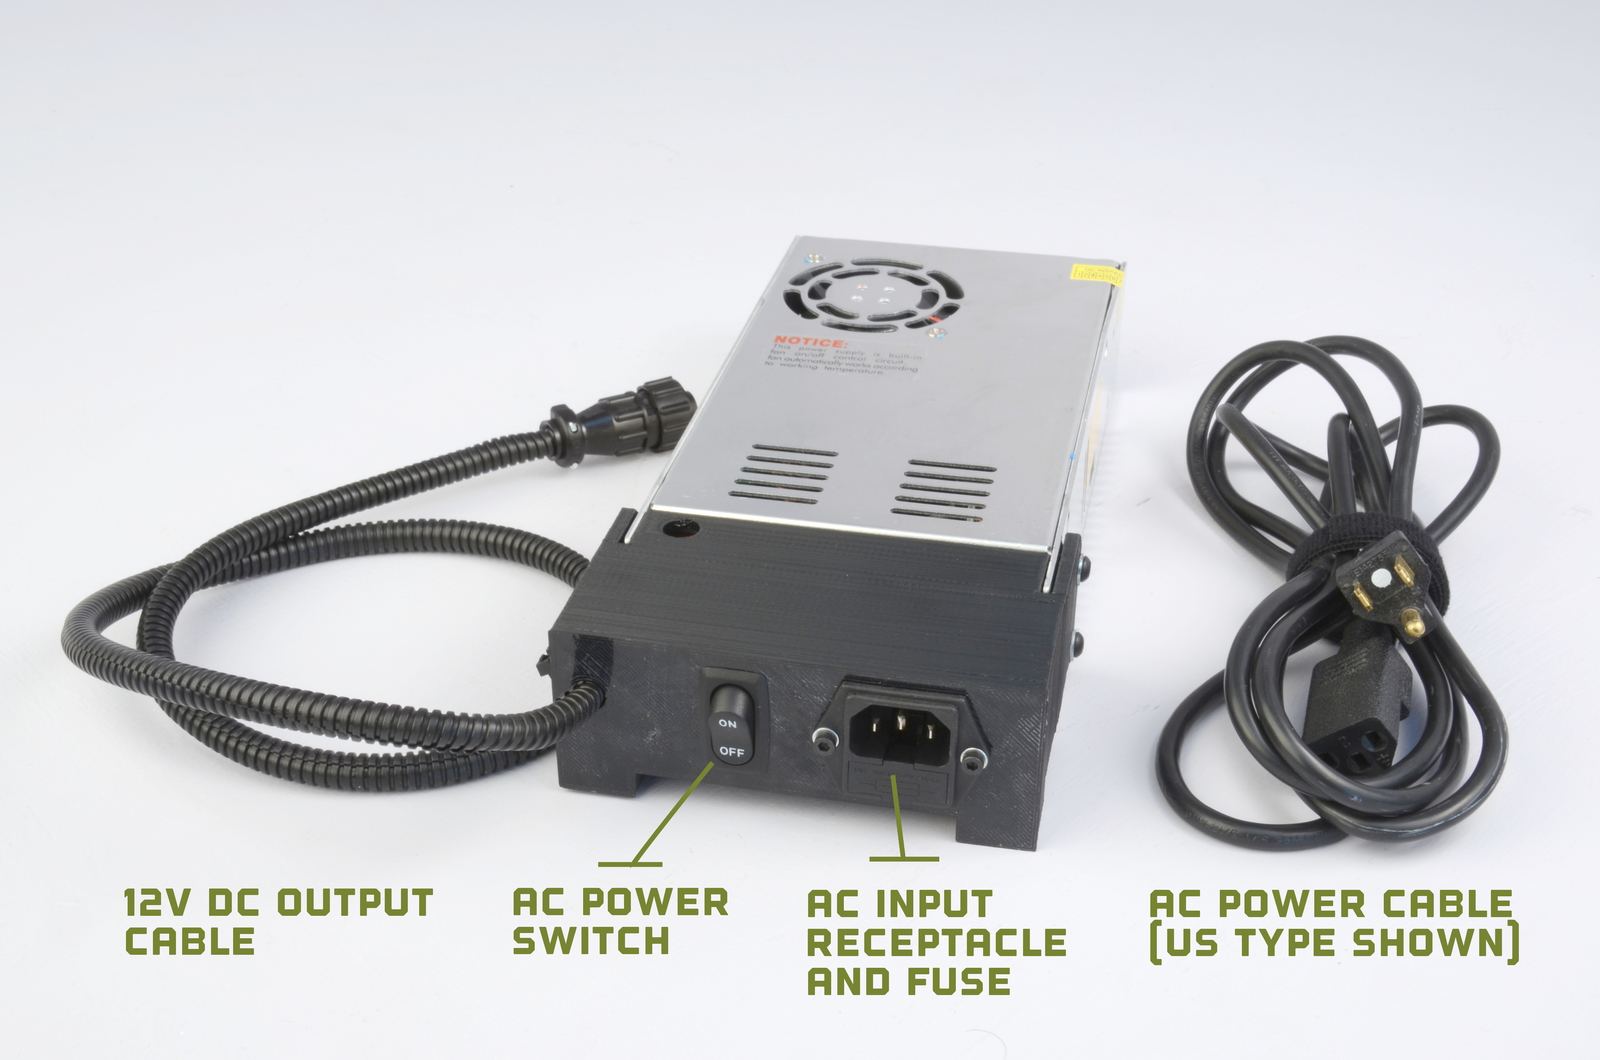
\includegraphics[keepaspectratio=true,angle=0,height=0.4\textheight,width=1.0\textwidth]{power_supply.JPG}
\caption{Power supply}
\label{fig:power_supply}
\end{figure}

%\begin{figure}[hp]
\begin{figure}[H]
\centering
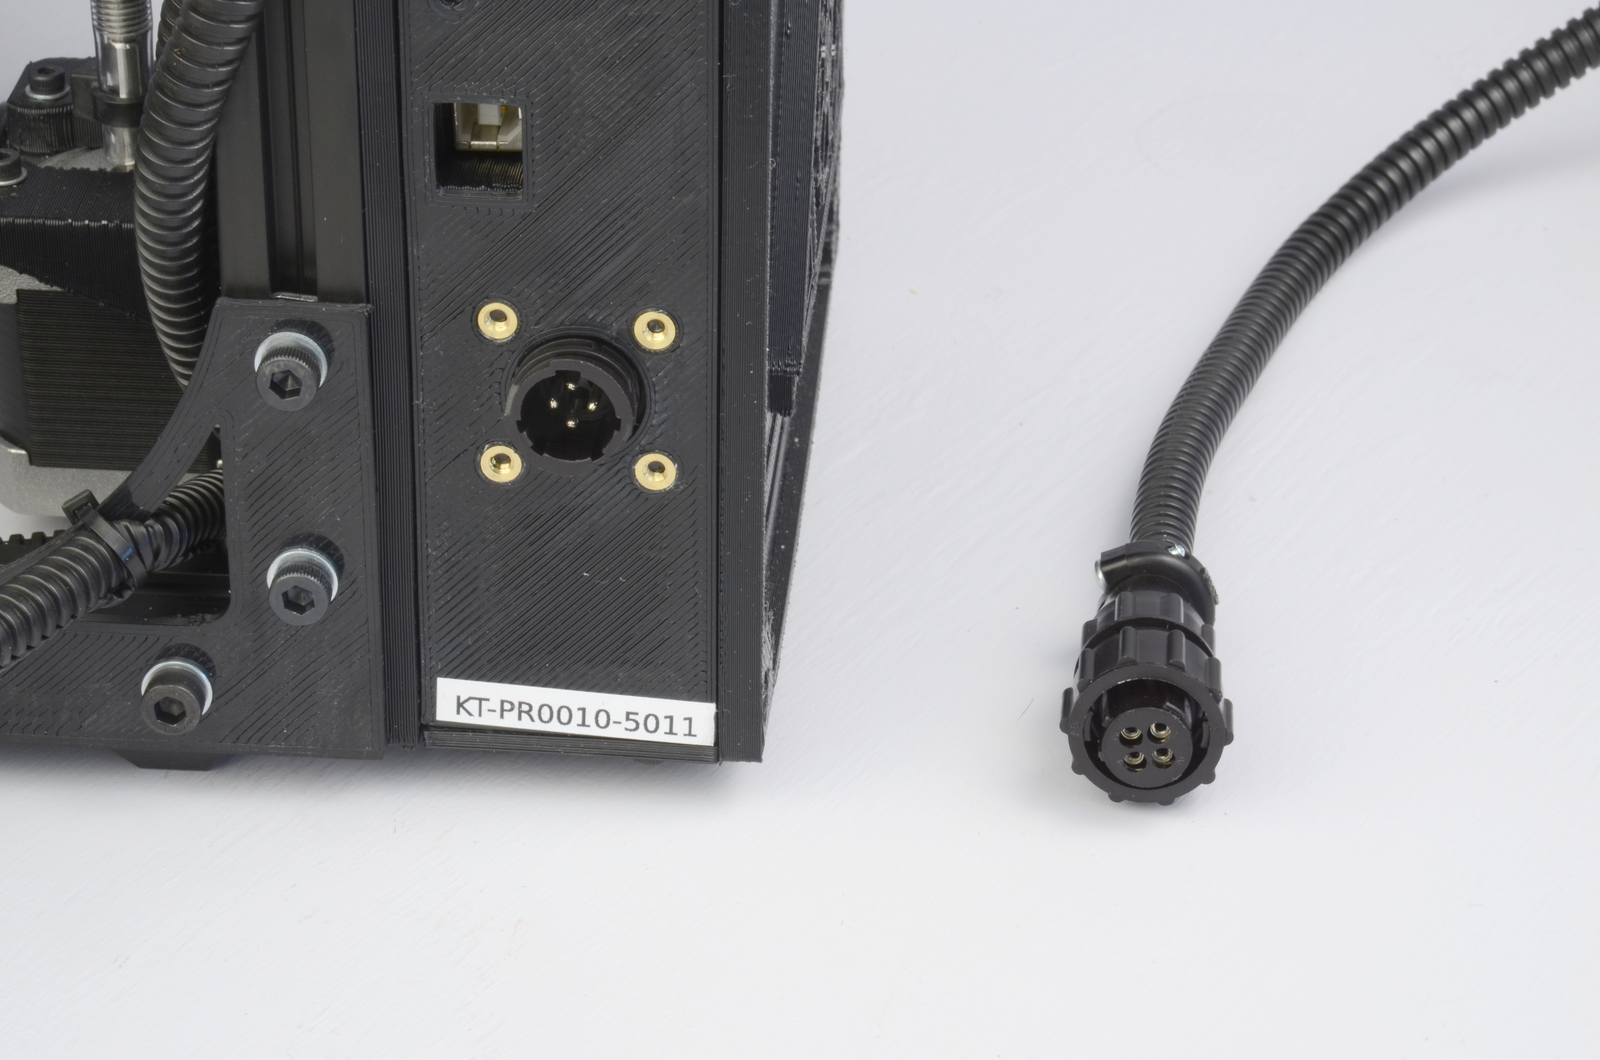
\includegraphics[keepaspectratio=true,angle=0,height=0.4\textheight,width=1.0\textwidth]{electronics_DC_connector.JPG}
\caption{12V DC Power supply plug and receptacle}
\label{fig:ps_plug}
\end{figure}

%\begin{figure}[hp]
\begin{figure}[H]
\centering
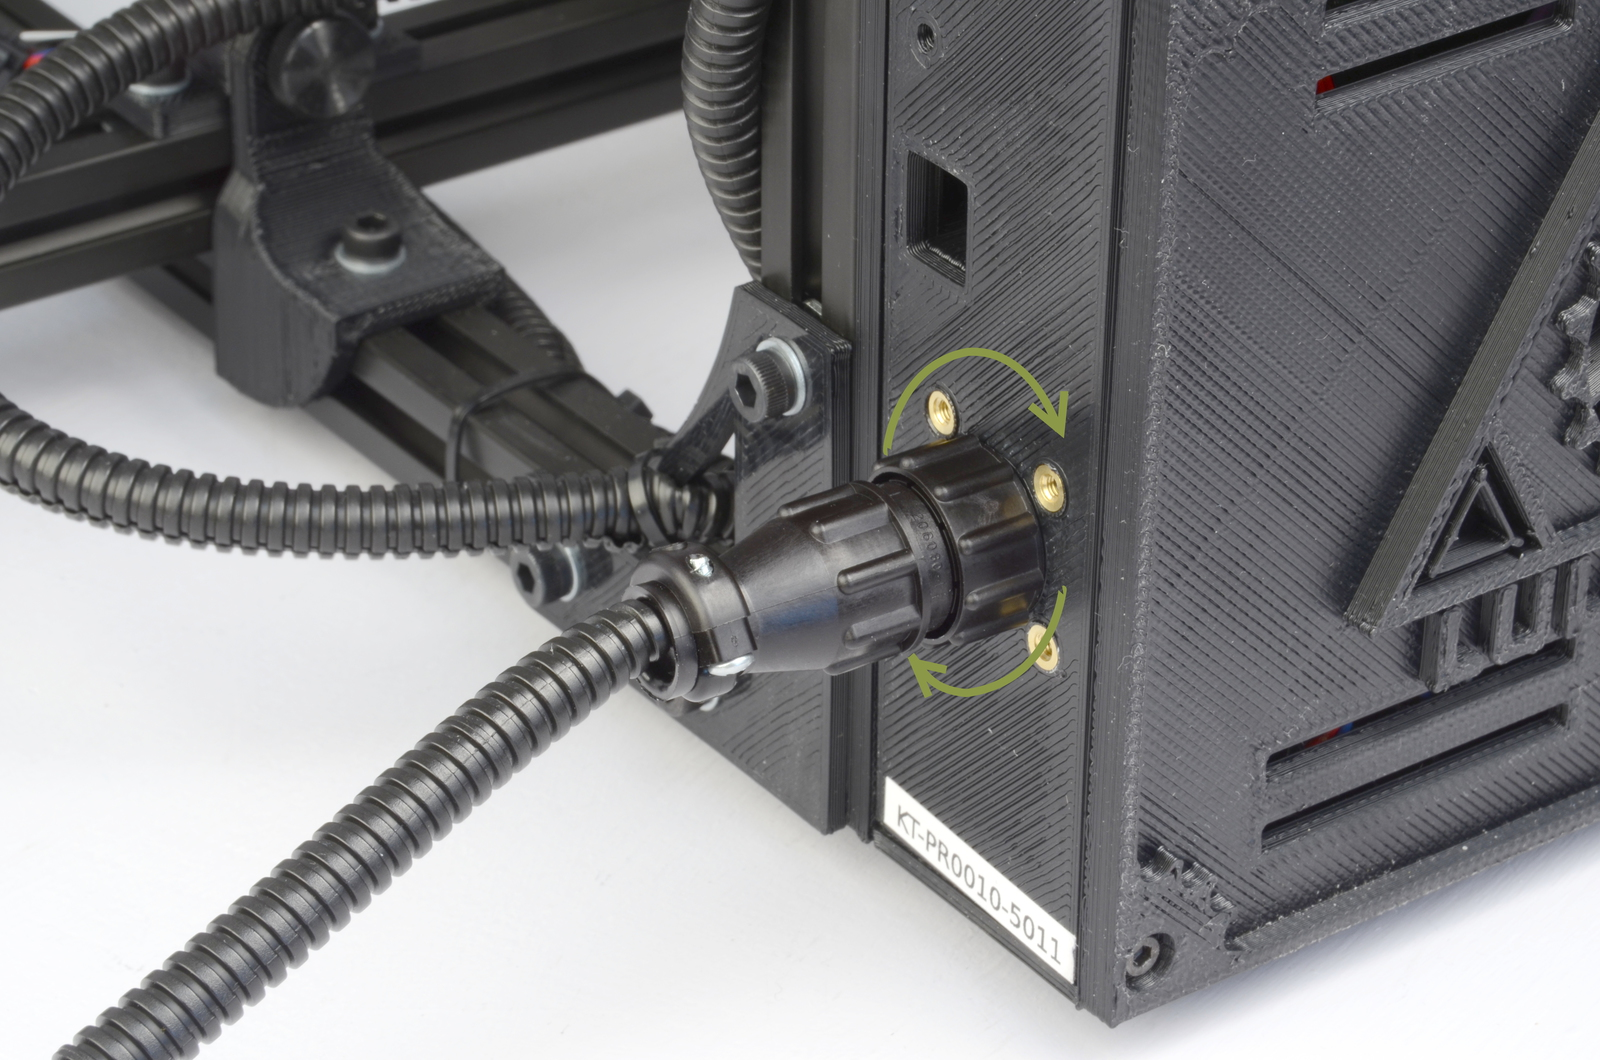
\includegraphics[keepaspectratio=true,angle=0,height=0.4\textheight,width=1.0\textwidth]{electronics_DC_connector_tight.JPG}
\caption{The power supply plug correctly plugged in}
\label{fig:electronics_plugs_plugged-in}
\end{figure}

\item Locate, on the right of the power supply, the red AC voltage switch. Depending on your location you will need to change the AC voltage switch to 115V or 230V. North America is generally 115V and the majority of other regions are 230V. You can find general voltage by country at \texttt{wikipedia.org/wiki/Mains\_electricity\_by\_country}.

\index{RAMBo}
\item Plug in the USB cable, B plug (square plug) side, into the USB receptacle on the printer electronics. Plug the other end of the USB cable, A plug side, into your computer.

\index{PTFE tube}
\item Locate the filament guide with attached PTFE tube
(Fig. \ref{fig:filament_guide}, page \pageref{fig:filament_guide}). The filament guide attaches to the filament guide mount which can be found on the top right side of the printer frame (Fig. \ref{fig:filament_guide_mount}, page \pageref{fig:filament_guide_mount}). The filament guide easily pops on to the guide mount as shown in figure \ref{fig:filament_guide_setting} (pg. \pageref{fig:filament_guide_setting}).
%\begin{figure}[hbt]
\begin{figure}[H]
\centering
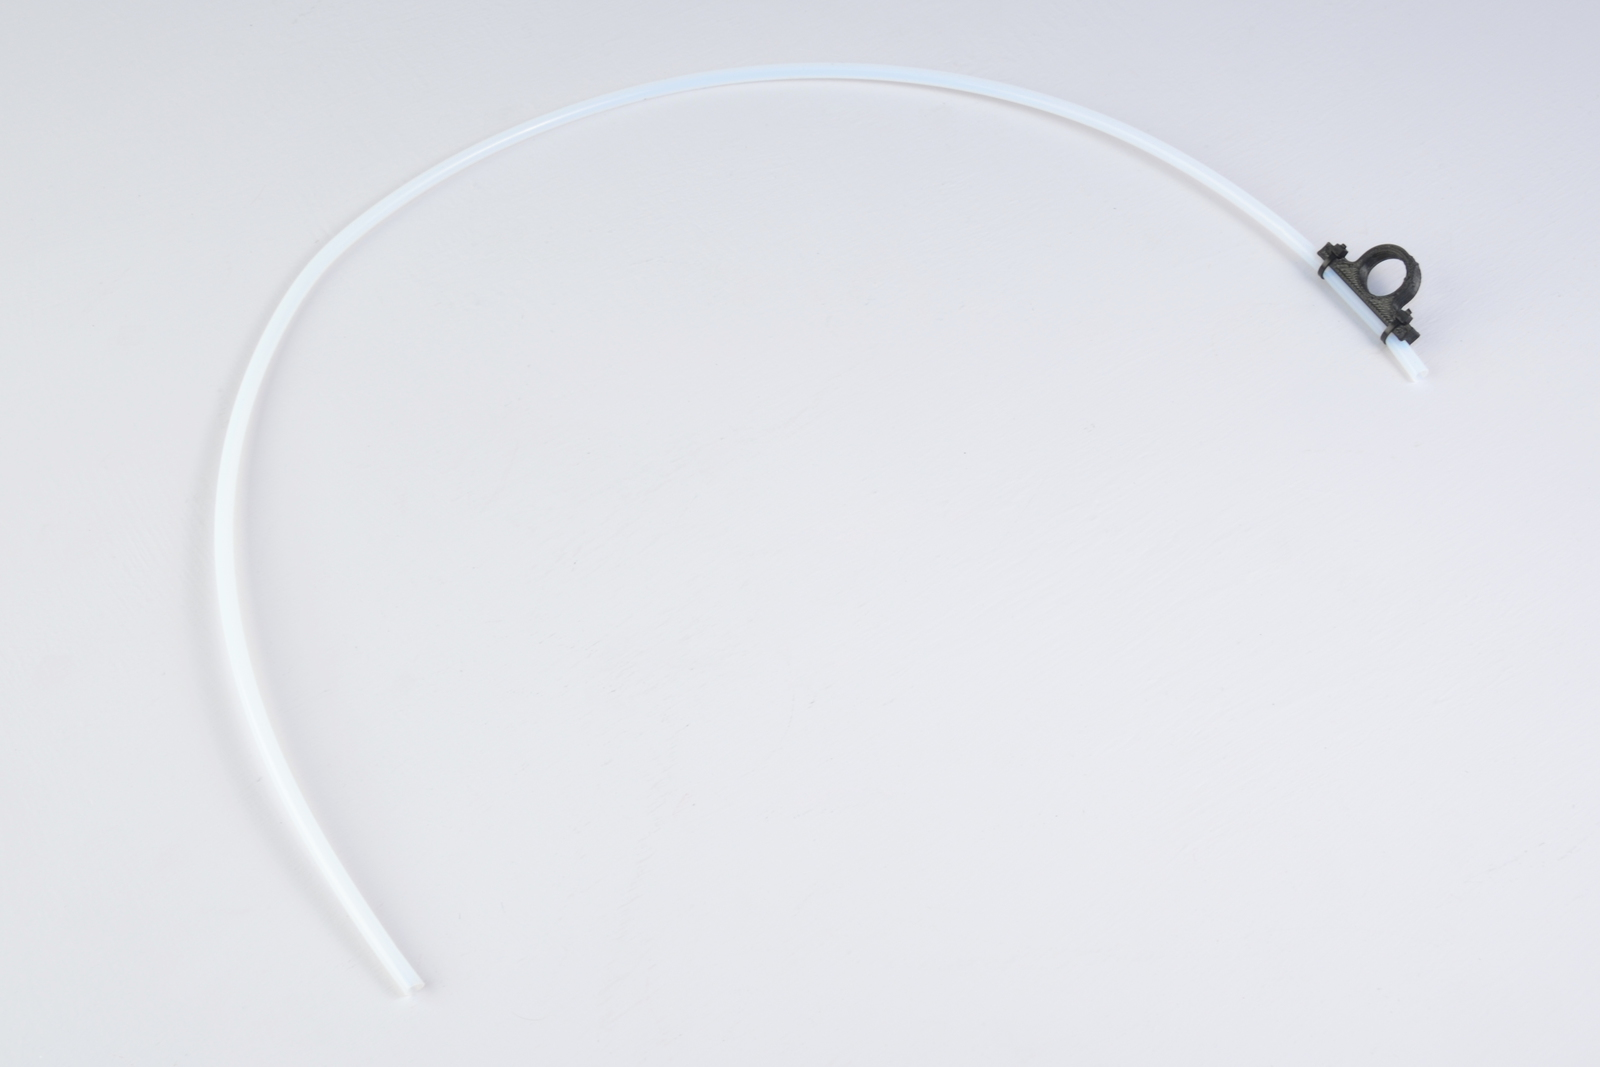
\includegraphics[keepaspectratio=true,angle=0,height=0.4\textheight,width=1.0\textwidth]{filament_guide.JPG}
\caption{Filament Guide}
\label{fig:filament_guide}
\end{figure}

%\begin{figure}[hbt]
\begin{figure}[H]
\centering
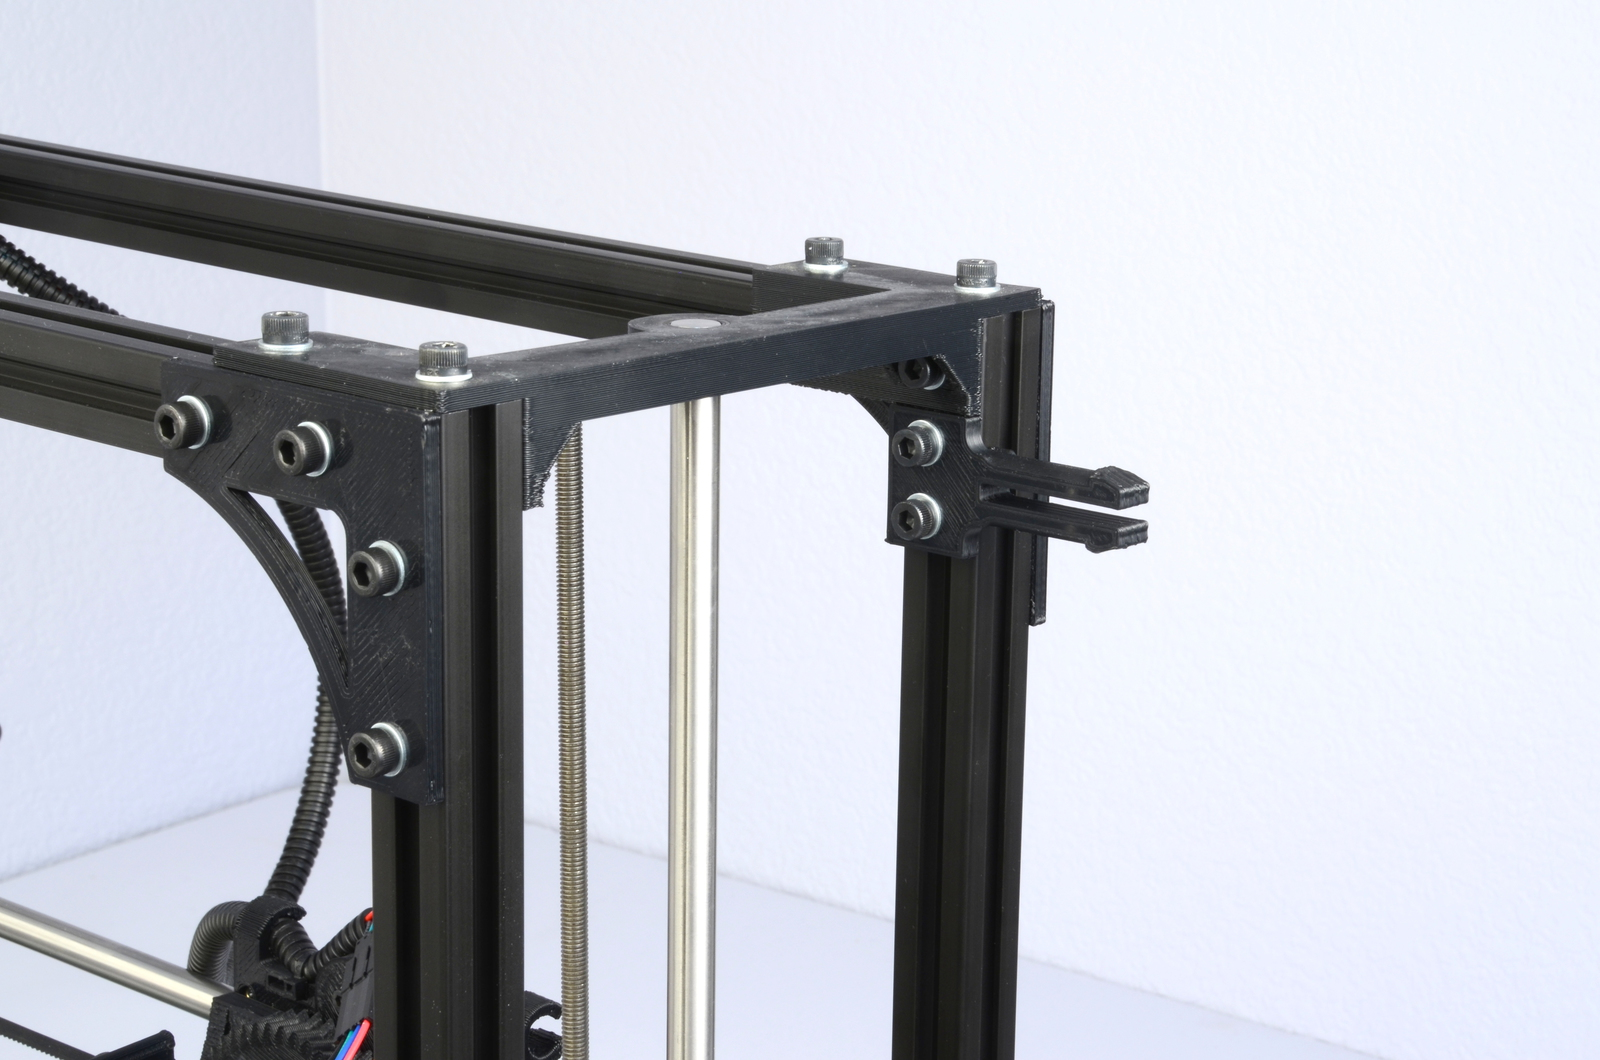
\includegraphics[keepaspectratio=true,angle=0,height=0.4\textheight,width=1.0\textwidth]{filament_guide_mount.JPG}
\caption{Filament Guide Mount}
\label{fig:filament_guide_mount}
\end{figure}

%\begin{figure}[hbt]
\begin{figure}[H]
\centering
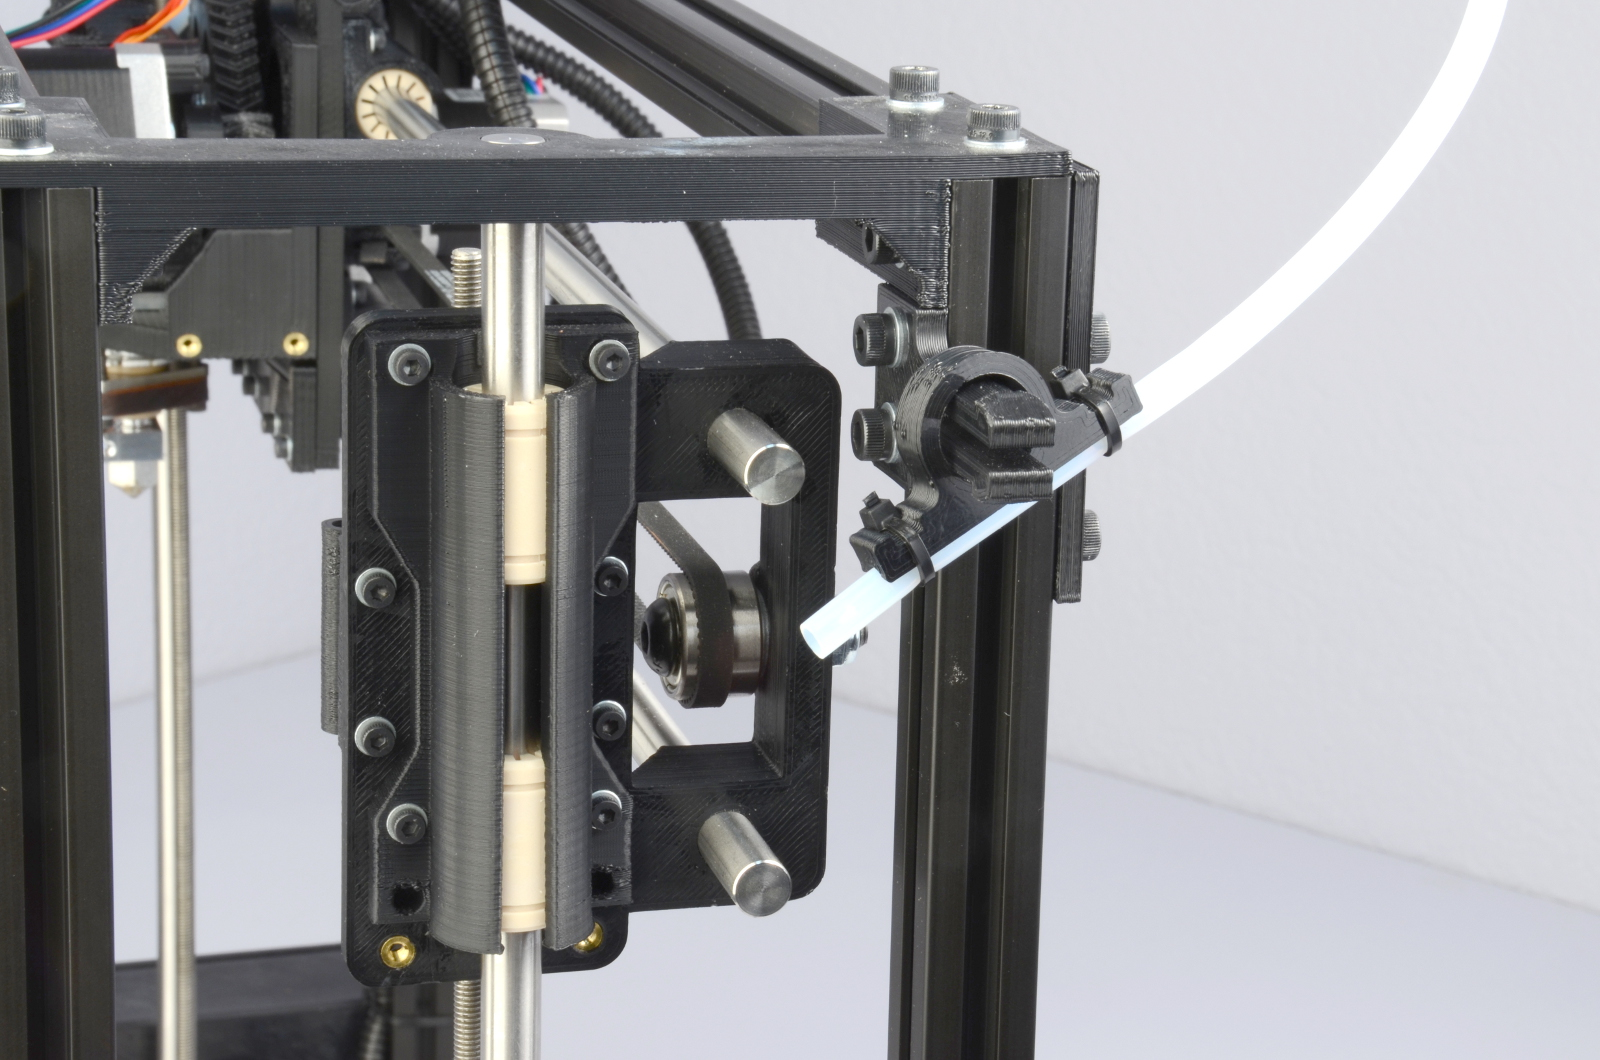
\includegraphics[keepaspectratio=true,angle=0,height=0.4\textheight,width=1.0\textwidth]{filament_guide_direction.JPG}
\caption{Filament Guide Setting}
\label{fig:filament_guide_setting}
\end{figure}

\index{end stops}
\glossary{End stops}{Mechanical or optical switches that are used to mark the 3 home (zero) positions.}
\item Your TAZ 3D printer is now setup and ready to start printing. Before moving forward you should become familiar with the TAZ Cartesian type system. The printer moves in three axes: X, Y, and Z (Fig. \ref{fig:axes}, page \pageref{fig:axes}). These three axes allow the tool head to move to any point within the print area. Note the location of the mechanical end stops which are small switches located at the home point of each axis (Fig. \ref{fig:endstops}, page \pageref{fig:endstops}). Each end stop switch allows the printer to find the 0, the origin, or starting point, of each axis. The mechanical end stops should never be blocked during the initial homing function or during a print.
%\begin{figure}[hbt]
\begin{figure}[H]
\centering
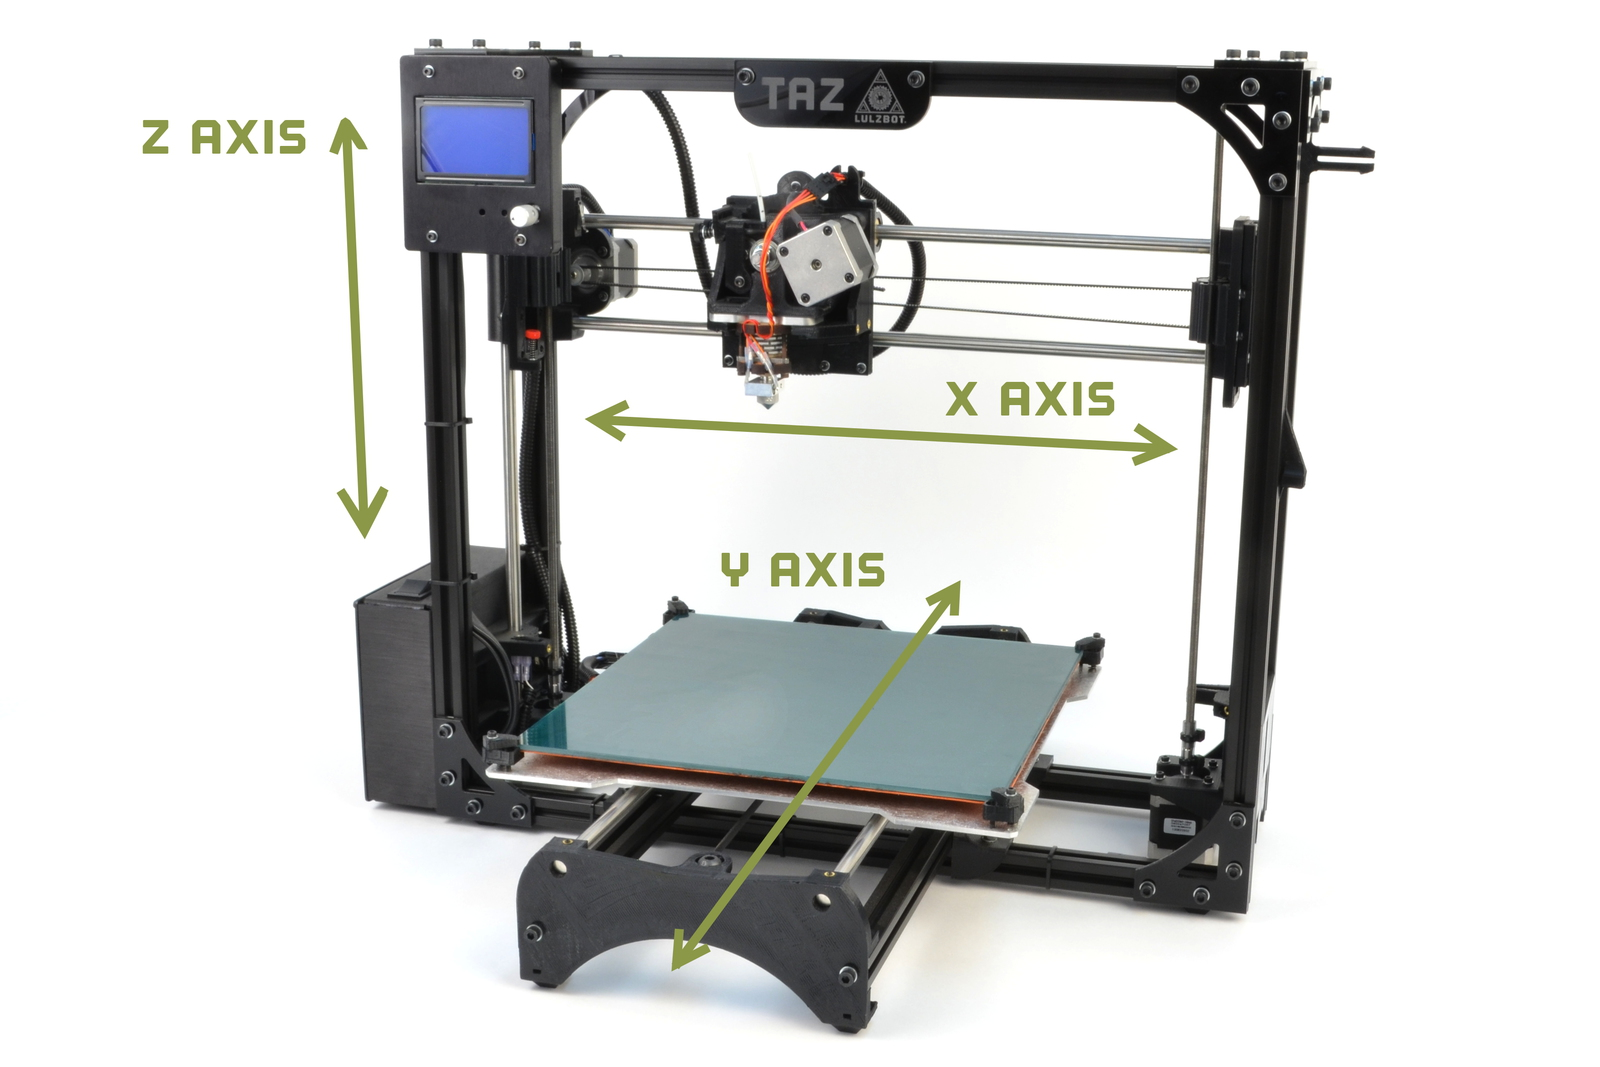
\includegraphics[keepaspectratio=true,angle=0,height=0.4\textheight,width=1.0\textwidth]{axes.JPG}
\caption{Axes movement directions}
\label{fig:axes}
\end{figure}

\begin{figure}[hp]
\centering
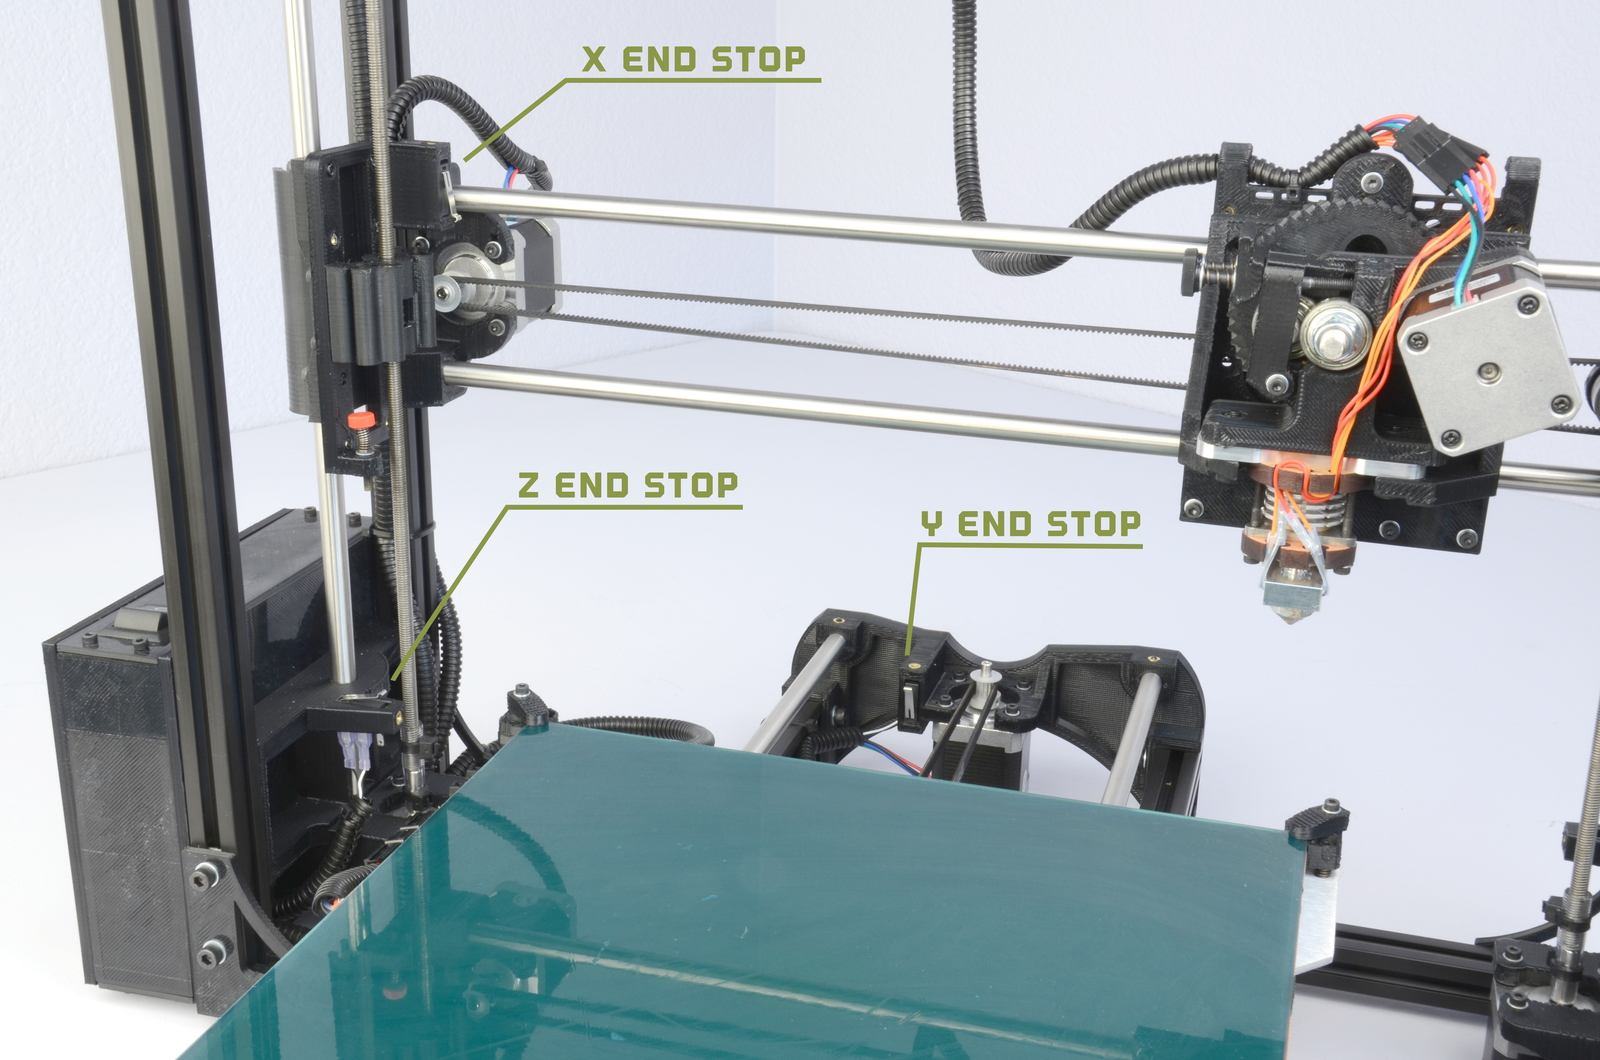
\includegraphics[keepaspectratio=true,angle=0,height=0.4\textheight,width=1.0\textwidth]{end_stop_switches.JPG}
\caption{End stop locations}
\label{fig:endstops}
\end{figure}

\end{enumerate}
}
\fi
%%% END SETUP %%%

%%% SOFTWARE %%%
\ifsoftware
\chapter{\emph{3D Printer Software}}
\thispagestyle{empty}
\markboth{3D Printer Software}{LulzBot\textsuperscript{\miniscule{\texttrademark}} TAZ User Manual}
{%
% Software.tex
%
% LulzBot® TAZ User Manual
%
% Copyright (C) 2015 Aleph Objects, Inc.
%
% This document is licensed under the Creative Commons Attribution 4.0
% International Public License (CC BY-SA 4.0) by Aleph Objects, Inc.
%

\section{\texttt{Software Overview}}
\index{software}

To operate your desktop 3D printer you will need to install a few software packages onto your PC. You will need a 3D printer host, an \texttt{.STL} to \texttt{.GCODE} generator, and optional CAD or 3D modeling software.

\texttt{Cura LulzBot\textsuperscript{\miniscule{\textregistered}} Edition is the recommended software for your LulzBot 3D printer.} Download Cura LulzBot Edition by visiting \texttt{LulzBot.com/Cura}.


\glossary{.GCODE}{The file extension for G-Code files}
\glossary{GCODE}{The common name for the most widely used CNC programming language.}
\glossary{CAD}{Computer Aided Design}

\index{GNU/Linux}
\index{OS X}
\index{Windows}
\index{operating system}
All of the following Free/Libre Software packages are available for GNU/Linux, Windows, and OS X. We highly recommend using these programs on GNU/Linux.

\section{\texttt{Software Types}}
\index{Printer Host}
\index{Slicing}
\index{Slicers}
\index{GCODE}
\index{g-code}

\begin{description}
\item{Printer Hosts} \hfill \\
Printer Host software is used to control the 3D printer. The program not only allows you to manually move the printer along all the axes, but set temperatures manually, send commands, and receive feedback/error messages from the onboard electronics. We recommend that new users start with Cura LulzBot\textsuperscript{\miniscule{\textregistered}} Edition as it includes a slicing engine as well.

\item{\texttt{Slicers}} \hfill \\
These programs take the 3-Dimensional model (typically STL/OBJ/etc) and determine the 3D printer toolpath based on the options selected. The slicing engine uses the nozzle diameter, movement speeds, layer height, and other variables to determine the coordinates where it needs to move, and the rates at which it will do so. This information is exported out of the program as a GCODE file. The GCODE file is a plain-text file with a series of text-based codes and a list of the complete X,Y, and Z-axis coordinates used for printing the 3D model. We recommend that new users start with Cura LulzBot Edition as it includes the printer host as well.

%Recommended Slicers:
%\begin{itemize}
%\item Cura LulzBot Edition
%\item Slic3r
%\item Skeinforge
%\item Sfact
%\end{itemize}

\end{description}

\index{download}
\index{driver}
\section{\texttt{Installing Drivers}}
GNU/Linux and OS X users will not need to install a driver to communicate with the LulzBot TAZ 3D printer. Windows users will need to install the drivers. Using Cura LulzBot Edition as your printer host and slicing software is recommended, as the drivers will automatically be installed during the Cura installation process. Download Cura LulzBot Edition by visiting \texttt{LulzBot.com/Cura}. The drivers can also be downloaded from \texttt{LulzBot.com/downloads}. A visual guide showing the driver installation process can be found in our download section as well.


\section{\texttt{CAD and 3D Modeling Software}}
\index{CAD}
\index{software}
\index{STL}

LulzBot is not distributing a CAD or 3D modeling software package. However, multiple Free/Libre Software packages are available. Other common non-free CAD and 3D modeling software are also capable of exporting the required \texttt{.STL} files.

On some CAD and 3D modeling software you will need to select millimeters as the output unit. If possible it is best to build your 3D design in metric units rather than imperial units. Cura requires .STL files sized in millimeters. If an .STL with inches as units is loaded into Cura, the model will be scaled much smaller than expected. You can scale the model by \texttt{25.40} to compensate. The software listed below outputs millimeters as the unit by default.

\subsection{\texttt{FreeCAD}}
\index{FreeCAD}
\index{GNU/Linux}
\index{Windows}
\index{OS X}
Website: \texttt{http://www.freecadweb.org/}

Although still in development, contains a full GUI for building CAD models. FreeCAD is capable of creating simple to complex designs. STL files can also easily be exported for use with 3D printing. FreeCAD is available for GNU/Linux, Windows, and OS X. The latest development version is recommended.

\subsection{\texttt{OpenSCAD}}
\index{OpenSCAD}
\index{GNU/Linux}
\index{Windows}
\index{OS X}
Website: \texttt{http://openscad.org}

OpenSCAD is different than FreeCAD in that it is script based. Rather than using a GUI to generate CAD designs, OpenSCAD CAD designs are created using script based renderings. Users with programming experience would find this useful. Also, OpenSCAD uses a simple script language that is easy for users with little or no programming experience to learn.

\subsection{\texttt{Blender}}
\index{Blender}
\index{GNU/Linux}
\index{Windows}
\index{OS X}
Website: \texttt{http://blender.org}

The most widely used Free/Libre Software 3D modeling software, Blender is well documented with tutorials available on the Blender.org website as well as found online.

\subsection{\texttt{Shapesmith}}
\index{Shapesmith}
Website: \texttt{http://shapesmith.net}

Shapesmith is a web-based 3D modeling software. This means there is no required software to get started designing models. Shapesmith is also a great choice for anyone starting out in CAD/ 3D modeling.

\section{\texttt{Alternative Printer Host Software}}
\index{Host}
\index{software}
\index{STL}

\subsection{\texttt{OctoPrint}}
\index{OctoPrint}
\index{GNU/Linux}
\index{Windows}
\index{OS X}
Website: \texttt{http://octoprint.org/}

Octoprint is a printer host that uses a web-based interface to access and control your 3D printer. Added web-cam functionality allows for time-lapse videos and a live stream. Octoprint will run on GNU/Linux, Windows, OS X based computers and can even run well on a Beagle Bone Black or a RaspberryPi (inexpensive business-card sized computers).

\subsection{\texttt{BotQueue}}
\index{BotQueue}
\index{GNU/Linux}
\index{OS X}
Website: \texttt{https://www.botqueue.com/}

BotQueue works well for those users wanting to have a web-based multiple 3D printer operation running off a queuing system.


\subsection{\texttt{MatterControl}}
\index{MatterControl}
%\index{GNU/Linux}
\index{Windows}
\index{OS X}
Website: \texttt{http://www.mattercontrol.com/}

MatterControl is another printer host that currently runs on GNU/Linux, Windows, and OS X. It features 2D and 3D model viewing, a print queue, and print file organization and searching.

\subsection{\texttt{Source Files}}
\index{Source Files}
Aleph Objects, Inc., the maker of the LulzBot\textsuperscript{\miniscule{\textregistered}} TAZ 3D printer, completely supports Free Software, Libre Innovation, and Open Source Hardware. Along with the LulzBot TAZ 3D printer being a Free Software and Open Source Hardware design, it has been tested to work with 100\% Free/Libre Software. Our source code and design files are hosted on:

\begin{description}
\item [LulzBot Download Server] \texttt{http://download.lulzbot.com}
\item [LulzBot Development Server] \texttt{http://devel.lulzbot.com}
\item [Aleph Objects Code Repository] \texttt{http://code.alephobjects.com}
\item [Aleph Objects Download Server] \texttt{http://download.alephobjects.com}
\item [Aleph Objects Development Server] \texttt{http://devel.alephobjects.com}
\end{description}

\glossary{Free Software}{Free Software (or Free/Libre Software) can be thought of as ``free as in free speech, not just free as in free beer'', although most Free Software is available for no cost. Free Software can be copied, modified and is freely available for download.}
\glossary{Libre Innovation}{Aleph Objects uses Free/Libre Software to build and improve Open Source Hardware so that everything we create is free to be viewed, copied, and/or modified by anyone.}
\glossary{Open Source Hardware}{Open source hardware is hardware whose design is made publicly available so that anyone can study, modify, distribute, make, and sell the design or hardware based on that design. The hardware source, the design from which it is made, is available in the preferred format for making modifications to it. For more information visit \texttt{http://www.oshwa.org/definition/}.}


}
\fi
%%% END SOFTWARE %%%

%%% FILAMENT %%%
\iffilament
\chapter{\emph{Loading Filament}}
\thispagestyle{empty}
\markboth{Loading Filament}{LulzBot\textsuperscript{\miniscule{\texttrademark}} TAZ User Manual}
{%
% Filament.tex
%
% LulzBot TAZ™ User Manual
%
% Copyright (C) 2015 Aleph Objects, Inc.
%
% This document is licensed under the Creative Commons Attribution 4.0
% International Public License (CC BY-SA 4.0) by Aleph Objects, Inc.
%

%%% Copy to Setup.tex, break at the point software is needed. %%%
\index{spool holder}
\index{filament arm}
\index{filament spool}
\index{spool}
\glossary{Spool}{Plastic filament coiled and stored on a plastic reel. Preferred over 1.75-mm filament due to improved feeding and better mounting options.}
\glossary{Filament}{Plastic material in a ``string'' like form, as it is fed to the printer.}
\glossary{ABS}{Acrylonitrile butadiene styrene thermoplastic. Usually extrudes at 230C.}
\glossary{PLA}{Polylactic acid is a corn-based biodegradable polymer. Usually extrudes at 185C.}
\glossary{HDPE}{High-density polyethylene.}
\glossary{Polycarbonate}{A strong and impact-resistant thermoplastic. Usually extrudes at ~300C.}
\glossary{HIPS}{High-impact polystyrene.}
\glossary{Laywoo-D3}{Wooden filament similar to PLA. Forty percent of its content consists of recycled wood. Usually prints at ~180C to 210C. Color can be changed by varying the extrusion temperature.}

Before you start printing you will need to load a reel of filament onto the filament arm. The filament arm is meant to work with 1-kg and 5-lb plastic filament reels but can be modified to work with other reel and spool types.

\begin{enumerate}

\item You will find the filament arm on the front right-hand side of the TAZ 3D printer (Figure \ref{fig:filament_arm}, page \pageref{fig:filament_arm}). Place the filament reel on the filament arm with the filament feeding counter-clockwise.

\begin{figure}[H]
\centering
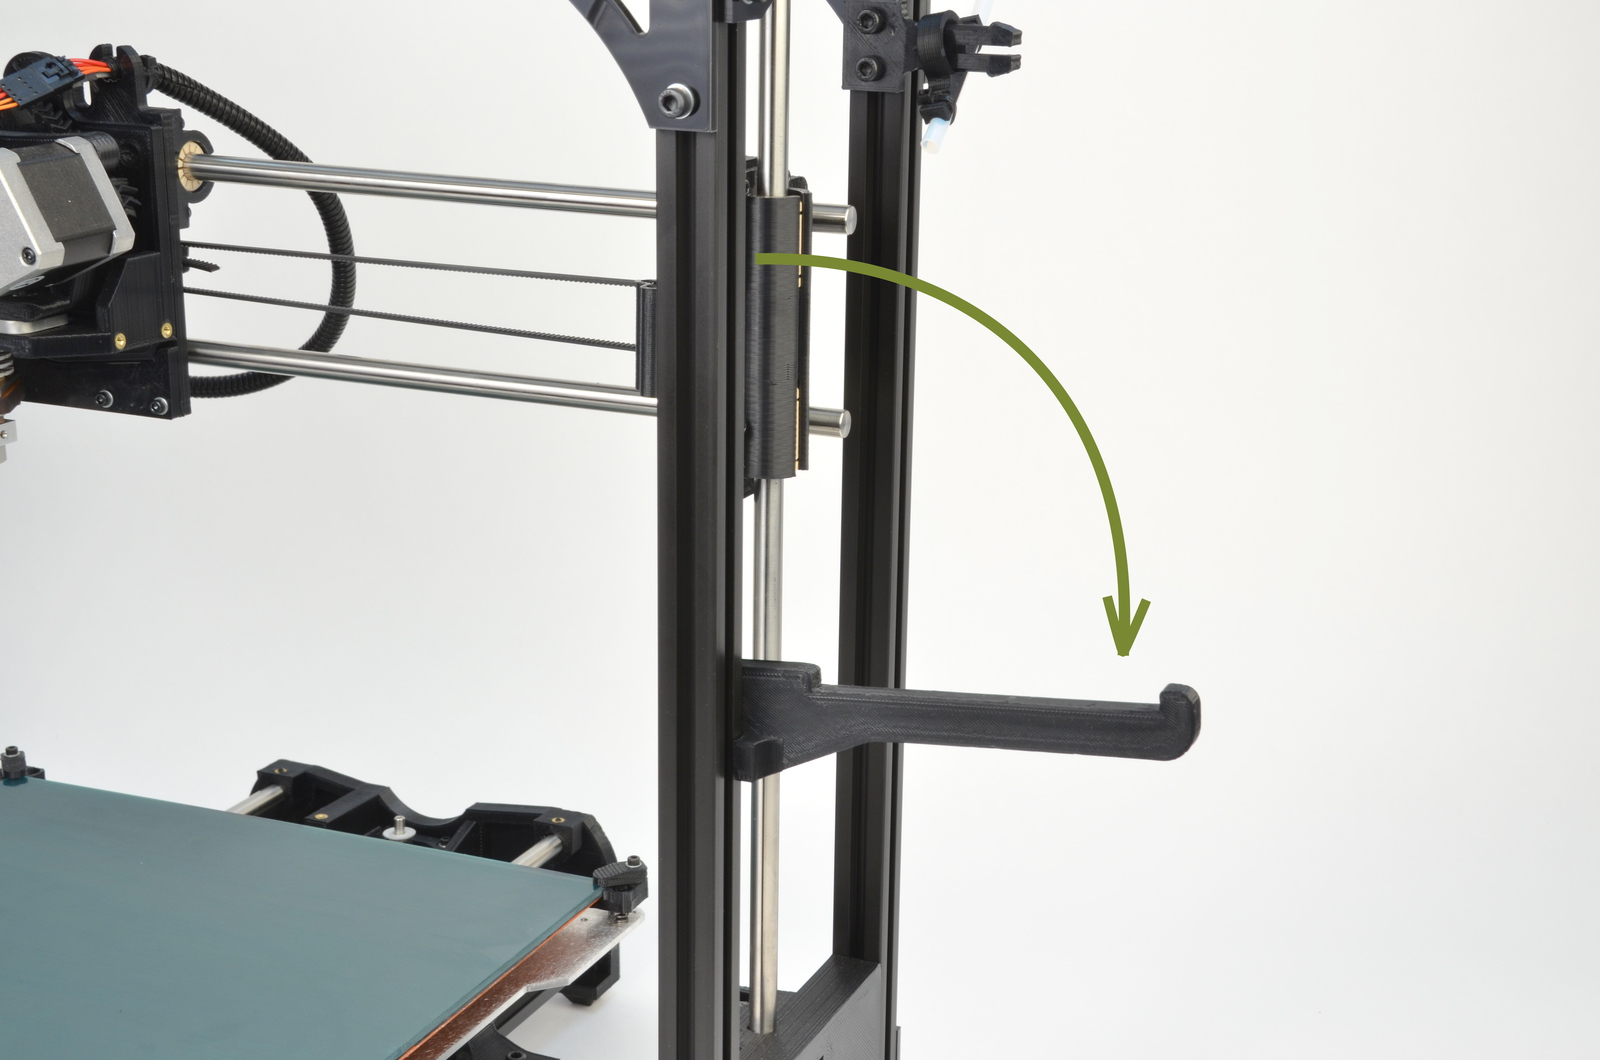
\includegraphics[keepaspectratio=true,angle=0,height=0.4\textheight,width=1.0\textwidth]{filament_arm.JPG}
\caption{Filament reel arm}
\label{fig:filament_arm}
\end{figure}

\index{feed tube}
\item Feed the end of the filament through the filament feed tube. The filament should now be threaded through the PTFE sleeve and exit near the extruder (Figure \ref{fig:filament_arm_loaded}, page \pageref{fig:filament_arm_loaded}).

\begin{figure}[H]
\centering
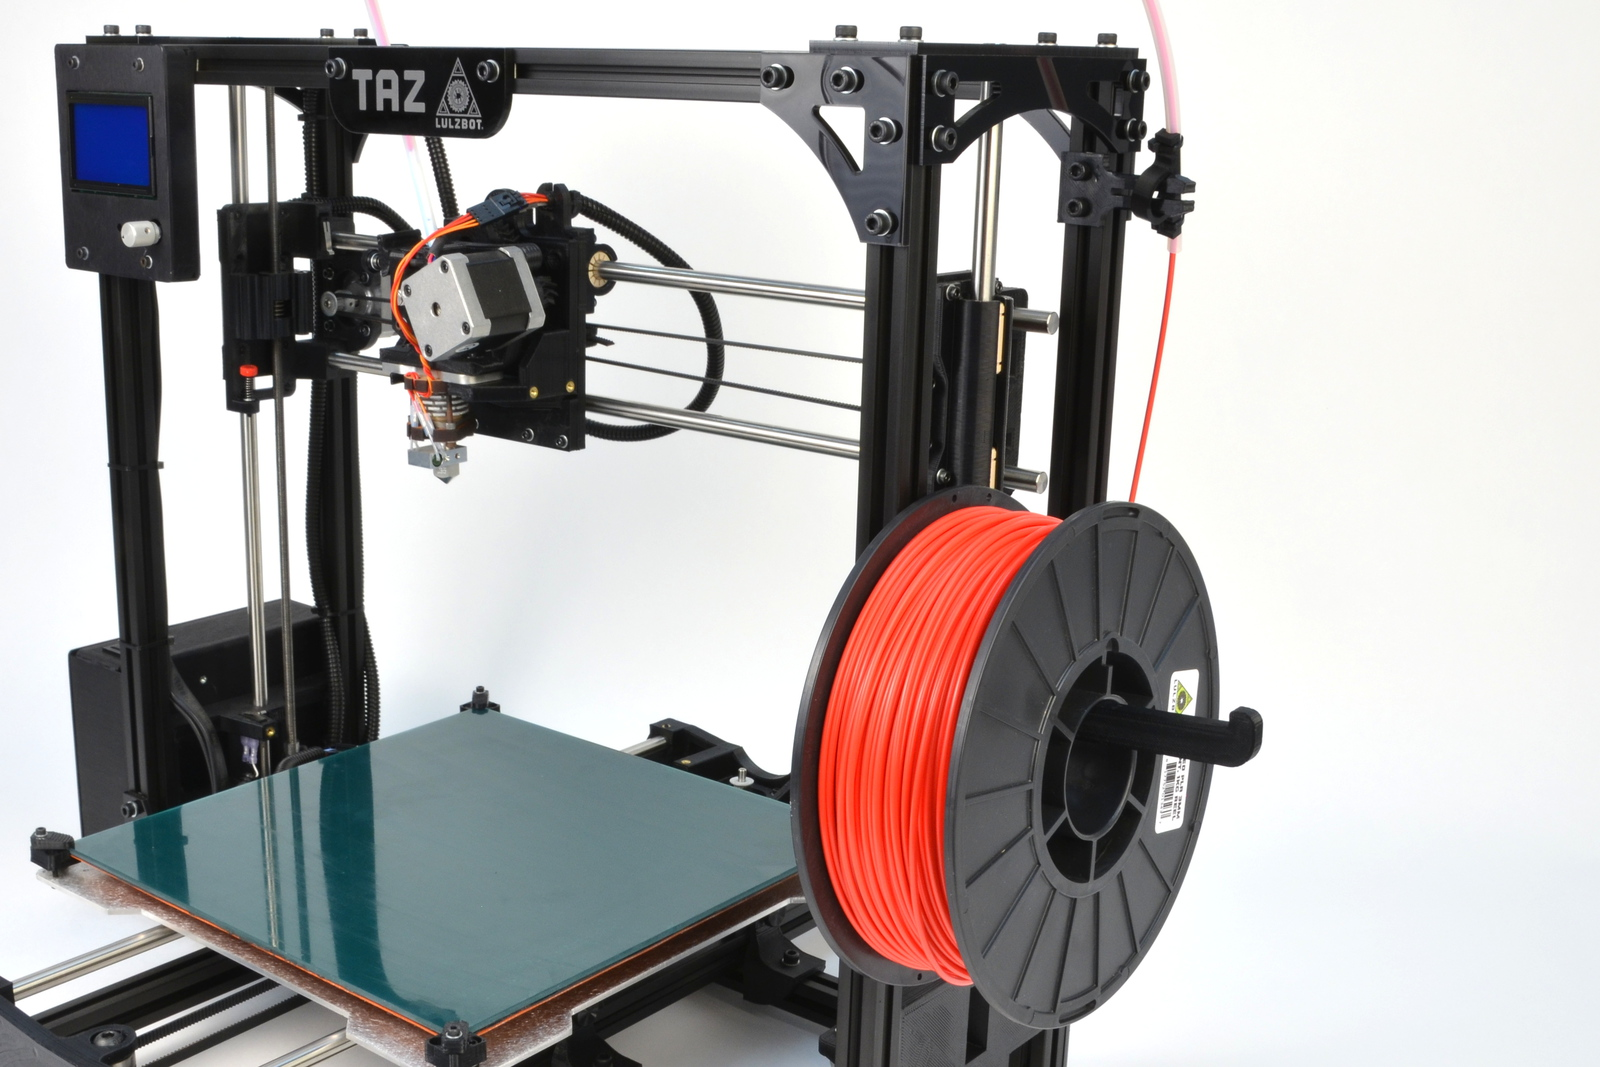
\includegraphics[keepaspectratio=true,angle=0,height=0.4\textheight,width=1.0\textwidth]{filament_arm_loaded.JPG}
\caption{Filament run through the guide}
\label{fig:filament_arm_loaded}
\end{figure}

\item Your filament reel is now mounted and ready for the next steps.

\item When changing filament, slide the opposite end of the filament through one of the holes in the hub of the filament spool. This will keep the filament from unwinding from the spool.

\end{enumerate}
}
\fi
%%% END FILAMENT %%%

%%% FIRSTPRINT %%%
\iffirstprint
\chapter{\emph{Your First 3D Print}}
\label{firstprint}
\thispagestyle{empty}
\markboth{Your First 3D Print}{LulzBot\textsuperscript{\miniscule{\texttrademark}} TAZ User Manual}
{\index{bed leveling}
\section{Bed Leveling}
Make sure you take the time to go through the following procedure to help ensure that your prints are consistent and trouble free. Make sure to first read the instructions for using the Printrun software. Connect to the printer as described in the Printrun software section. Once \texttt{Pronterface} is connected to the printer use the homing buttons to home the X and Y axis. \textcolor{red}{Do not use the \texttt{Home Z button} until after the \texttt{Z axis End stop} has been adjusted. Make sure that the red shipping clamps on the Z axis smooth rods have been removed before continuing.}

\subsection{Rough Adjustment of the Z Axis End Stop Trigger}
\index{end stop}
\begin{figure}[H]
\centering
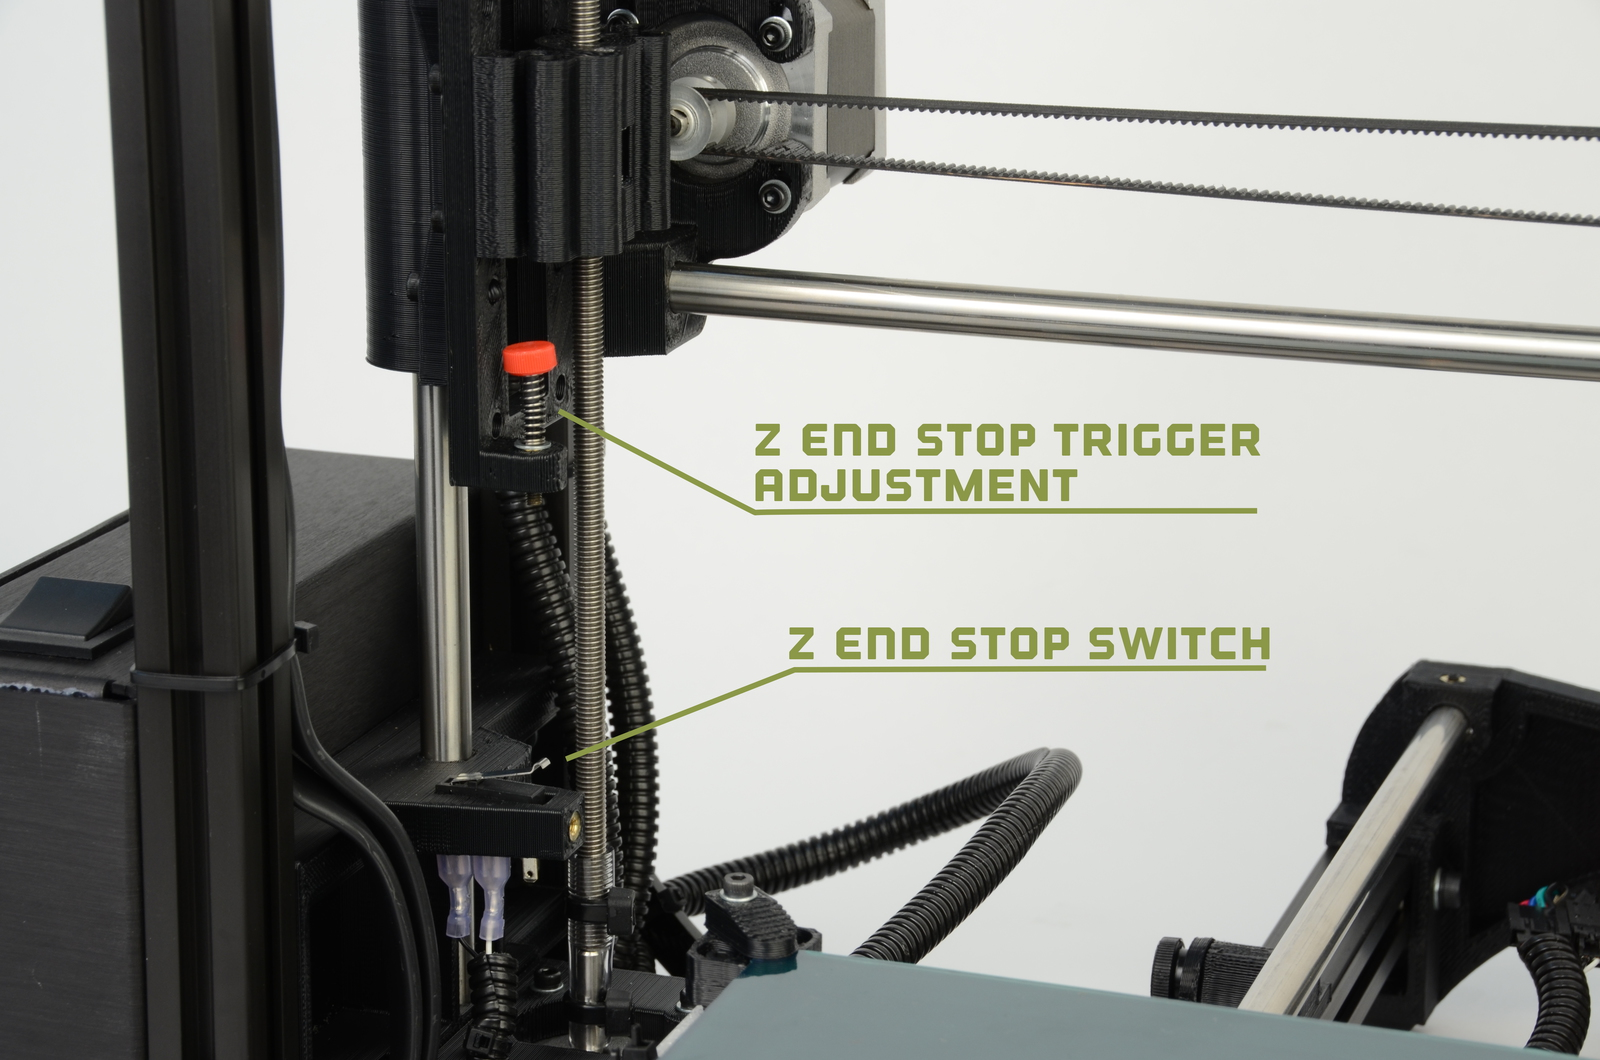
\includegraphics[keepaspectratio=true,angle=0,height=0.4\textheight,width=1.0\textwidth]{Z_end_stop_trigger.JPG}
\caption{Z end stop trigger}
\label{fig:Z_end_stop_trigger}
\end{figure}
To lower or raise the Z home height adjust the Z end stop trigger. The red end stop trigger is on the far left of the printer mounted on the X-axis motor mount. Before using the \texttt{home Z} button or the \texttt{home all} button you will need to adjust the \texttt{Z axis endstop trigger}. Once connected to the TAZ 3D printer in Pronterface, Rotate the \texttt{Z axis end stop trigger} clockwise to lower the bottom of the screw closer to the Z axis end stop. Once lowered by approximately 1cm, press the \texttt{HomeZ button} to home the Z axis. The hot end will approach the heated bed and should stop around a centimeter above the surface of the heated bed. While the Z axis is moving down pay attention to the Z axis movement and sound. The Z axis stepper motors should be moving in unison. If you notice a grinding sound stop, turn the printer off and before proceeding, make sure that the Z axis looks level in relation to the body of the TAZ 3D printer. Manually rotate one of the Z axis stepper motors by hand if needed to visually level the Z axis.

\index{z axis}
\subsection{Raising the Z Axis}
Use the \texttt{+Z 10 button} to move the Z axis up in \texttt{10mm} increments. \textcolor{red}{Commands sent in Pronterface will stack, so multiple movement button presses can potentially be harmful and cannot be stopped without powering down the 3D printer.} Keep an eye on the nozzle for the hot end. Raise the Z axis until the hot end nozzle is approximately 40-50mm away from the print bed.

\subsection{Verify Z Axis Leveling}
With the Z axis above the bed, use the included \texttt{150mm ruler} to measure the distance from the bottom of the \texttt{X axis} smooth rod and the top surface of the \texttt{Y axis} aluminum bed plate on the left side.
\begin{figure}[H]
\centering
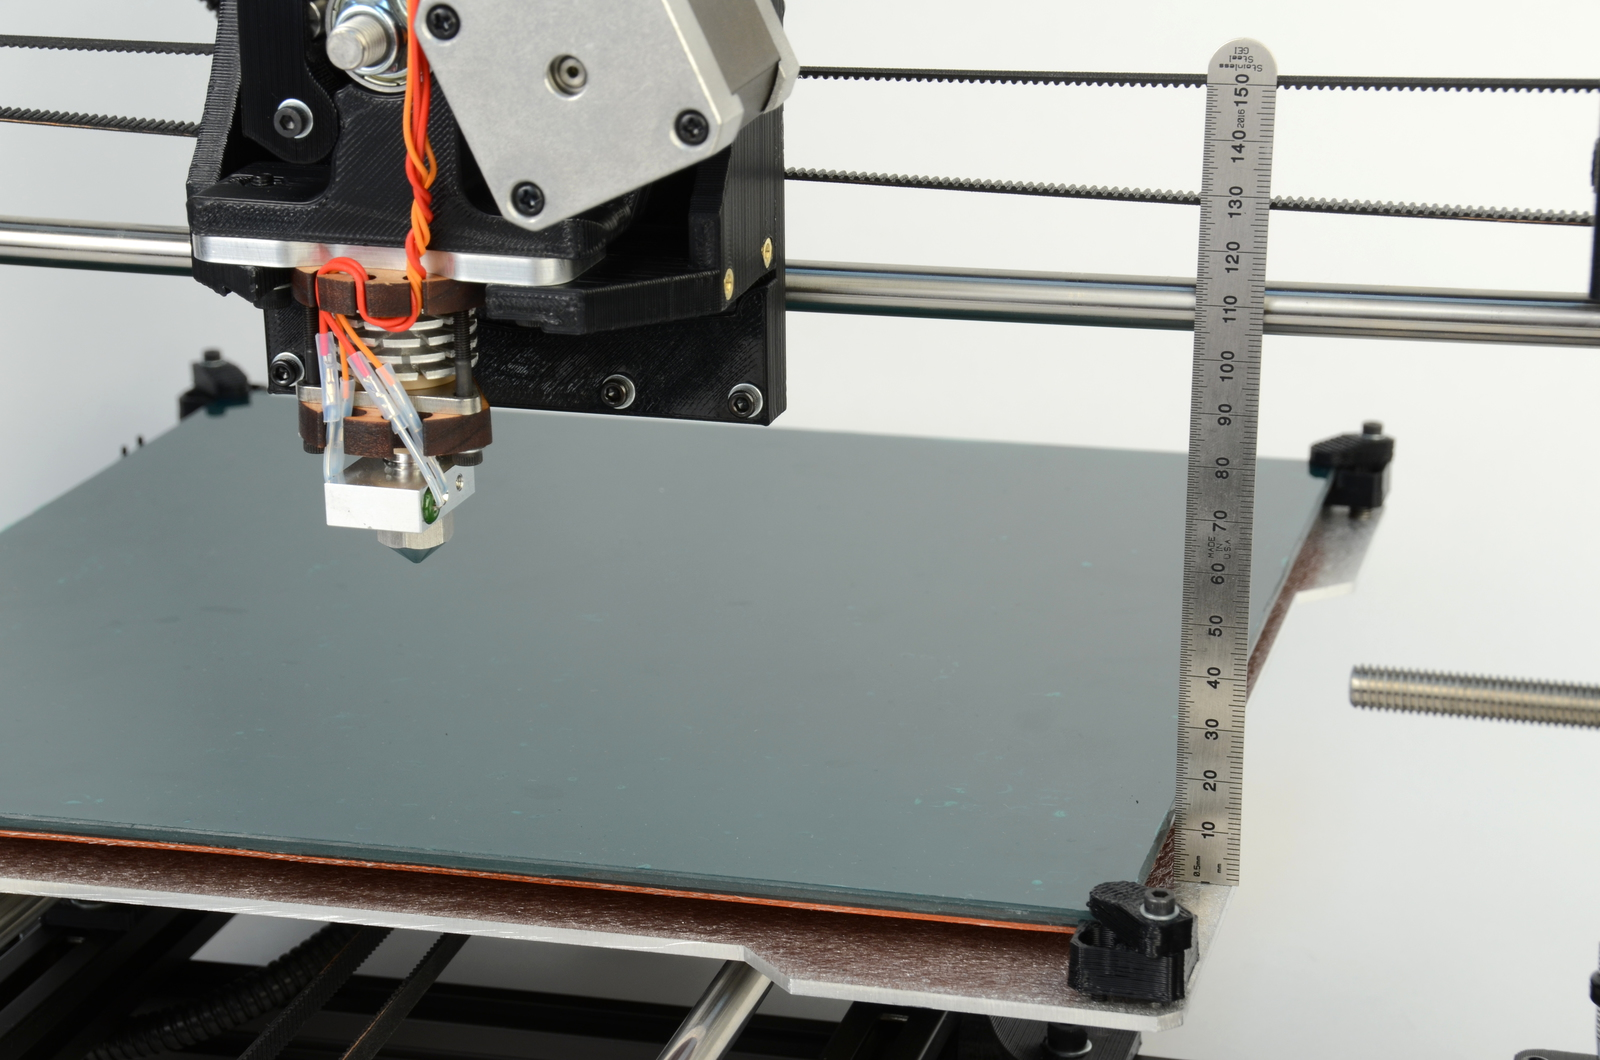
\includegraphics[keepaspectratio=true,angle=0,height=0.4\textheight,width=1.0\textwidth]{X-Y_axes_leveling_check.JPG}
\caption{Verifying the X and Y axis are square}
\label{fig:X-Y_axes_leveling_check}
\end{figure} 
Compare the distance measurement from the left side to the measurement on the right side. The distance measurement should be the same. If not, in Pronterface use the \texttt{Motors off} button to turn off the stepper motors on the TAZ 3D printer. Manually, by hand, turn the threaded rod on one side of the printer to raise or lower that side to match the measurement on the other side. If the Z axis has been adjusted measure again to confirm that the left and right side of the Z axis are level in relation to the Y axis aluminum plate.


\subsection{Fine Adjustment of the Z Axis End Stop}
\begin{comment}
\begin{figure}[H]
\centering
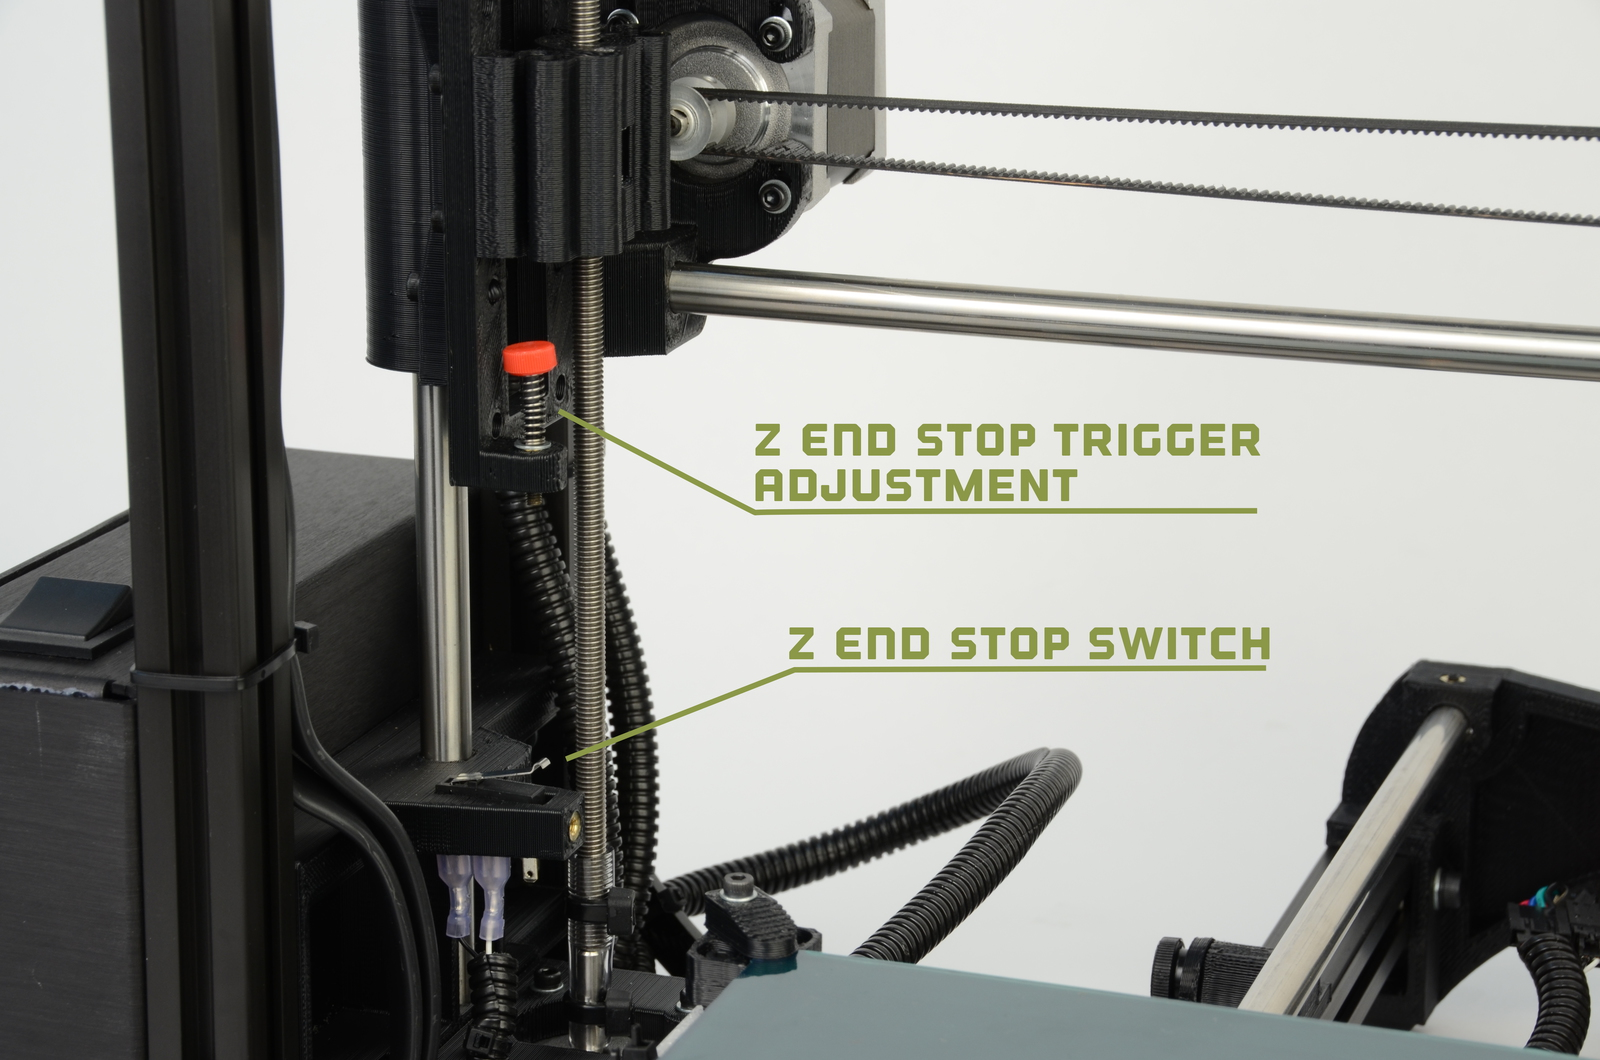
\includegraphics[keepaspectratio=true,angle=0,height=0.4\textheight,width=1.0\textwidth]{Z_end_stop_trigger.JPG}
\caption{Z end stop trigger}
\label{fig:Z_end_stop_trigger}
\end{figure}
\end{comment}
To lower or raise the Z home height adjust the Z end stop trigger. The red end stop trigger is on the far left of the printer mounted on the X-axis motor mount.
Adjust the \texttt{Z axis end stop trigger} by rotating the screw counter-clockwise to raise the tip of the screw. Raise the screw by roughly the same amount of the distance between the nozzle tip and the print surface. Press the \texttt{Home Z} button to home the Z axis. The tip of the nozzle should now be very close to the surface of the bed.

\subsection{Leveling the Print Bed}
Slide a thin piece of paper underneath the nozzle in the front left corner of the bed. Adjust the Z axis end stop and home the Z axis until the tip of the nozzle applies a firm pressure on the paper. Try to slide the paper from underneath the tip of the nozzle. It should not tear, but some resistance should be felt. Move the hot end nozzle tip over to the far side of the X axis by using the \texttt{+X 100 button}. As the X axis carriage approaches the end of the X axis use the \texttt{+X 10 button} and finally the \texttt{+X 1 button}. Once the tip of the nozzle is near the front right corner of the bed slide the same piece of paper under the nozzle and home the Z axis. To raise or lower the front right corner of the bed adjust the third screw from the left. Do not adjust the middle screw. Adjust the front right corner of the bed until the amount of tension felt when moving the piece of paper under the nozzle feels the same as the tension felt when doing the same thing on the front left corner. Repeat the same process using the \texttt{+Y button} to move the heated bed to place the nozzle on the rear right corner of the bed. Adjust the height of the bed using the same procedure as outlined above. Finally, move the X axis carriage over to the rear left corner of the bed and perform the same leveling procedure to adjust the last corner. The bed should now be almost perfectly level. We will check this in a later section. Use the controls in Printrun to raise the Z axis up 20mm, and move the X axis carriage over to the center of the X axis.

\section{Set Temperature}
\index{temperature}
%Make sure to first read the instructions for using the Printrun software. Connect to the printer as described in the Printrun software section
%%% XXX pageref going to \label not \section (page \pageref{Installing Printrun}).
Set the hot end and print surface for ABS or PLA plastic and turn both on. The temperature settings for ABS should be set at \texttt{230°C} for the hot end and \texttt{85°C} for print surface; for PLA they should be set at \texttt{185°C} for the hot end and \texttt{55°C} for print surface. Click the \texttt{Motors Off} button.
\glossary{Idler}{Refers to parts using a bearing (usually a 608ZZ) to add tension in belts or to add pressure against a rolling surface.}
\section{Load Filament}
\index{filament}
\index{hot end}

Once the hot end is heated to the correct temperature you will now need to load the plastic filament into the extruder.
\begin{figure}[hbt]
\centering
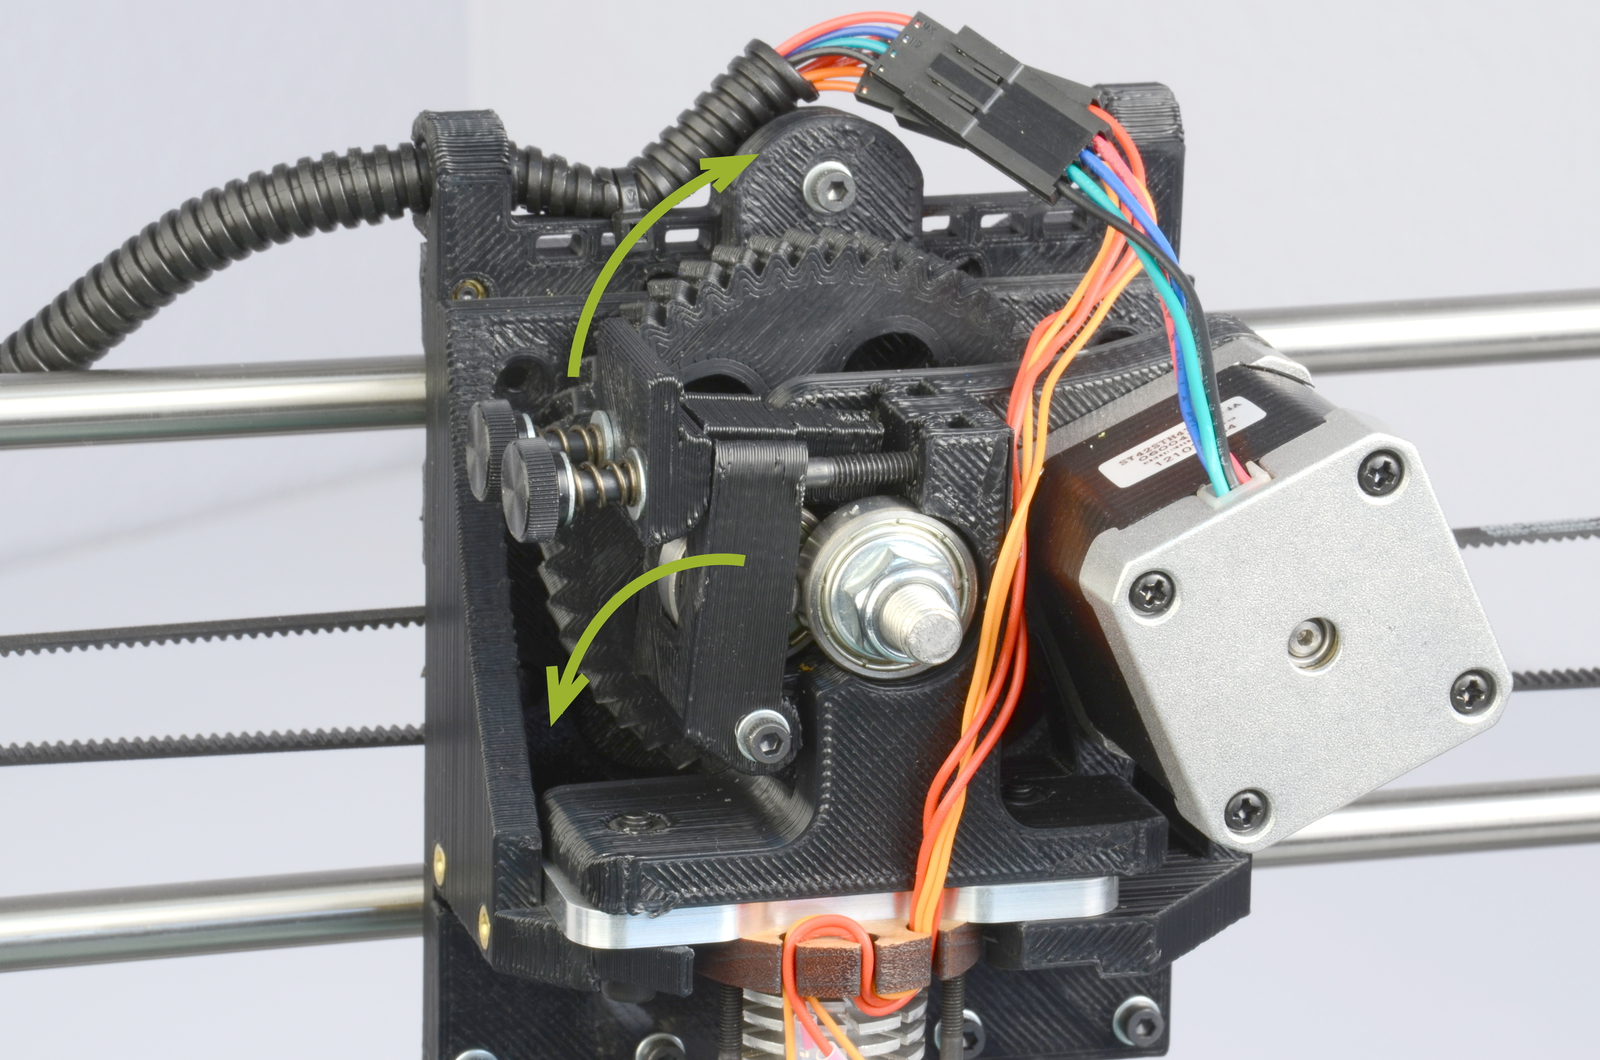
\includegraphics[keepaspectratio=true,angle=0,height=0.4\textheight,width=1.0\textwidth]{extruder_idler_release.JPG}
\caption{Extruder idler release}
\label{fig:extruder_idler_release}
\end{figure}
% update feed hole picture.
Gently squeeze both the idler screws and the plastic clip together and pull upwards to release the idler (Fig. \ref{fig:extruder_idler_release}, page \pageref{fig:extruder_idler_release}). The idler screws can be loosened if necessary. The idler can be rotated downwards allowing access to the hobbed bolt and filament feed hole(Fig. \ref{fig:extruder_filament_slot}, page \pageref{fig:extruder_filament_slot}). If the extruder has a small section of filament already loaded, you will need to remove the filament once the extruder idler has been opened, by gently pulling out the filament by hand once the hot end has reached extrusion temperature. From the previously installed filament reel, feed the end of the plastic filament into the filament feed hole
(Fig. \ref{fig:extruder_filament_slot}, page \pageref{fig:extruder_filament_slot}).
\begin{figure}[hbt]
\centering
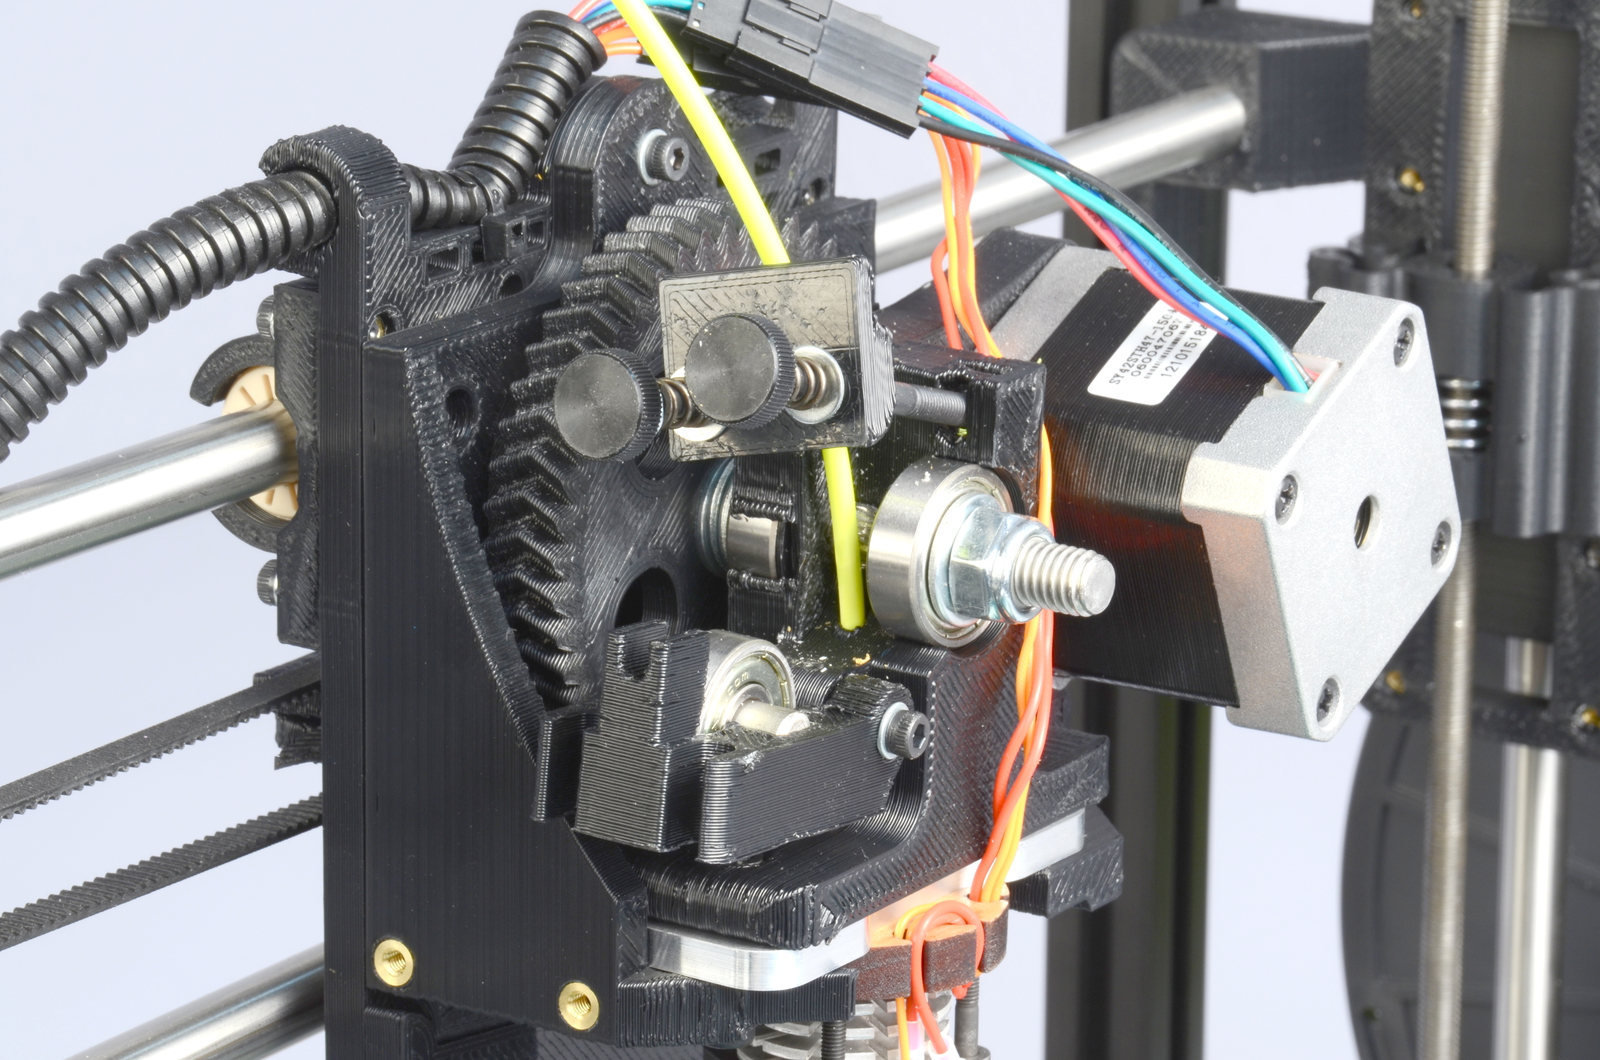
\includegraphics[keepaspectratio=true,angle=0,height=0.4\textheight,width=1.0\textwidth]{extruder_filament_slot.JPG}
\caption{Extruder filament slot}
\label{fig:extruder_filament_slot}
\end{figure}
Now you can push the filament through the extruder by slowly pushing the filament down into the hot end.

Once the filament extrudes a small amount out of the nozzle raise the idler and slide the two idler bolts and plate back into place. Tighten the two idler bolts if you previously loosened them. Tighten the two screws until they are finger tight, then tighten them slightly more. Now use the \texttt{Extrude} button in Printrun to test that the extruder is working properly. You may need to extrude 40-60mm of filament to fully prime the hot end. Adjust the tension on the two screws until you can reliably and repeatedly extrude roughly 40mm of filament.

\section{Home Printer}
Use the home buttons to home the X axis and then the Y axis. Next home the Z axis. When the Z axis is at home the nozzle tip should be right above the glass
(Fig. \ref{fig:nozzle_height}, page \pageref{fig:nozzle_height}). The image to the left, in figure \ref{fig:nozzle_height}, is the correct nozzle height.
\begin{figure}[p]
\centering
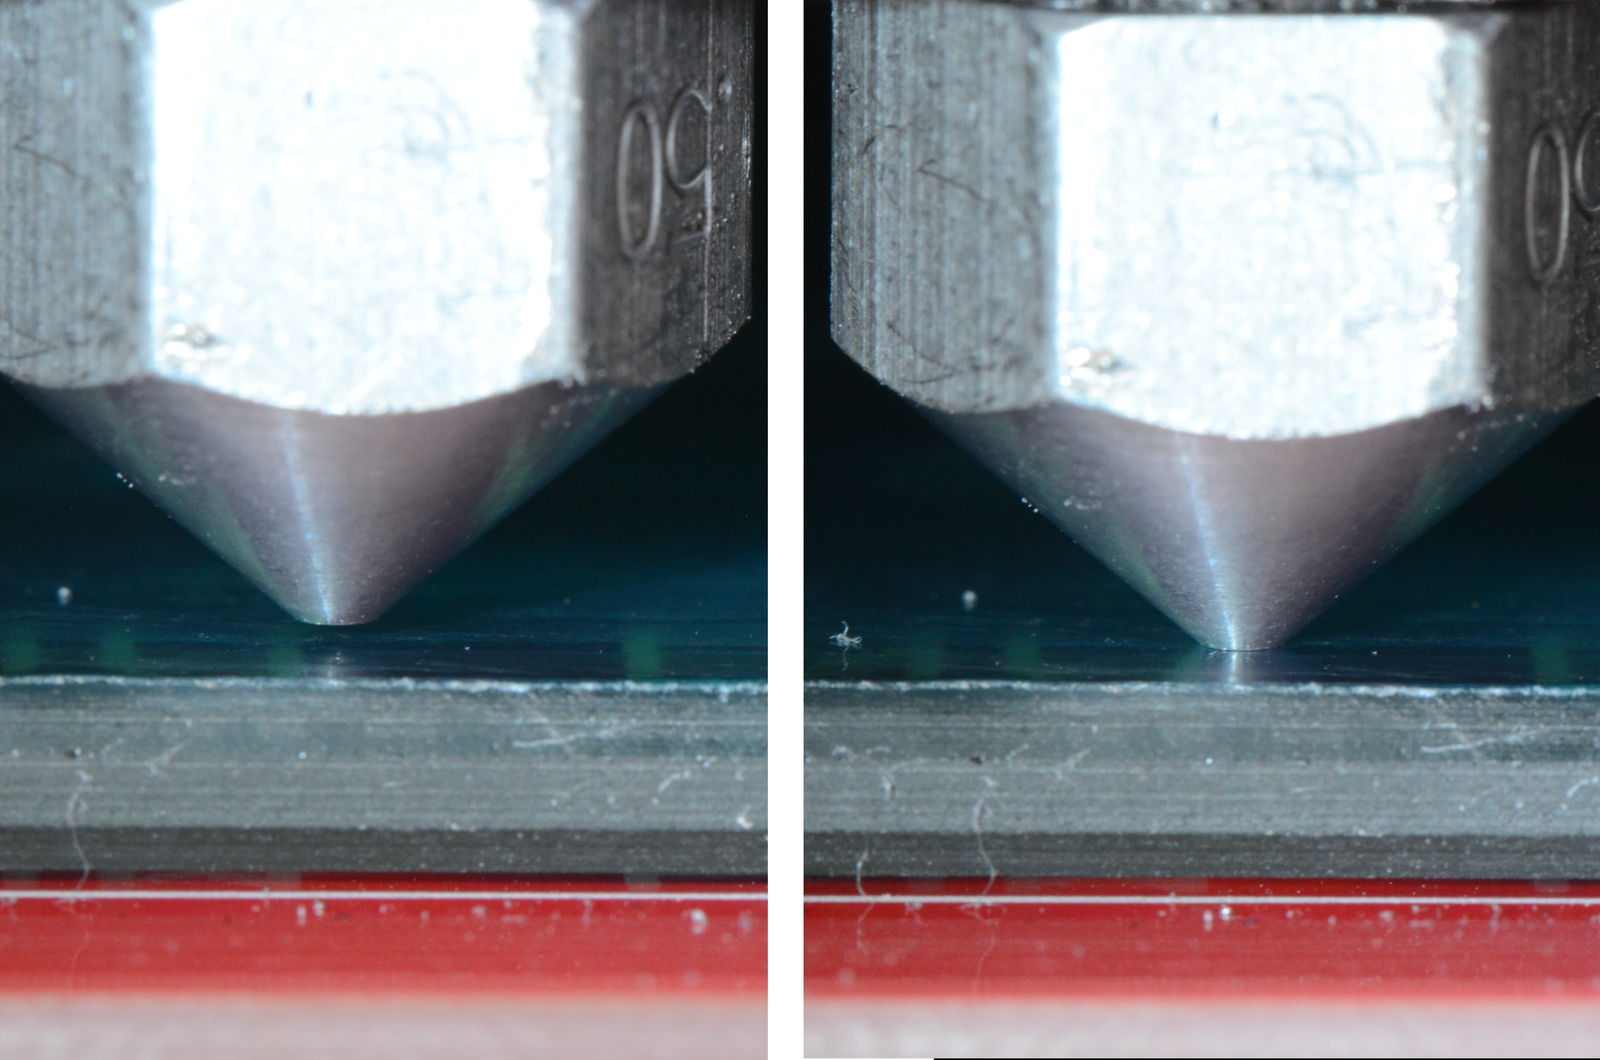
\includegraphics[keepaspectratio=true,angle=0,height=0.4\textheight,width=1.0\textwidth]{nozzle_height.jpg}
\caption{Nozzle height}
\label{fig:nozzle_height}
\end{figure}
\begin{figure}[p]
\centering
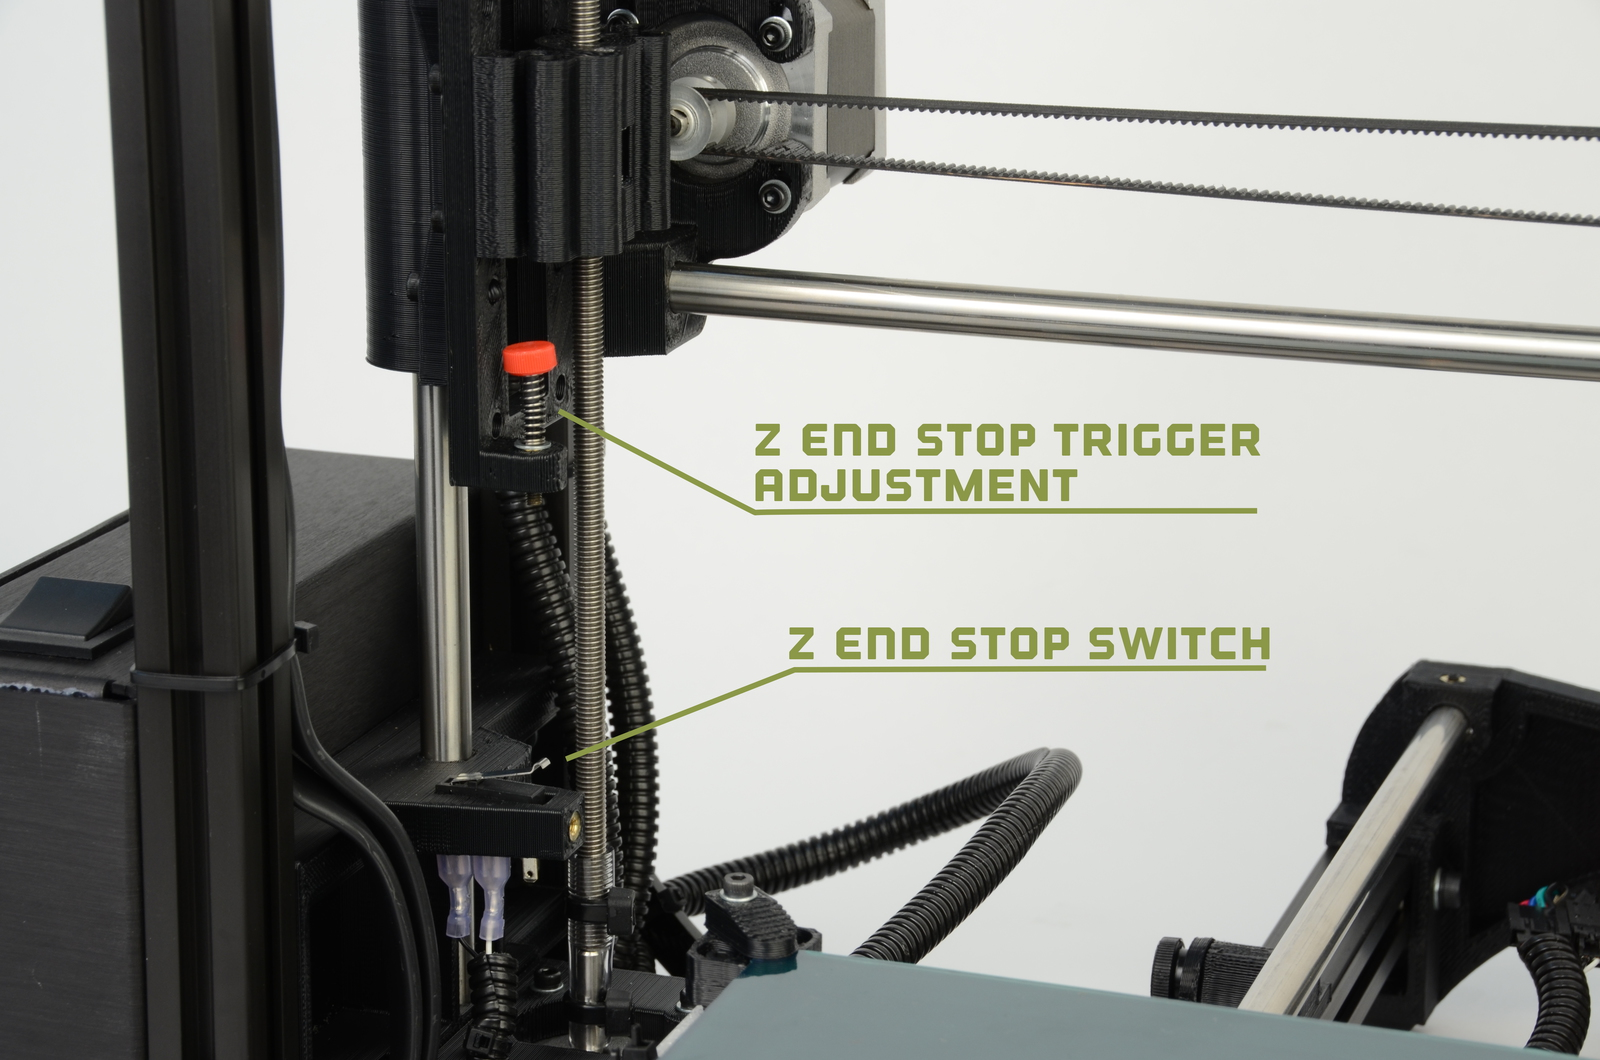
\includegraphics[keepaspectratio=true,angle=0,height=0.4\textheight,width=1.0\textwidth]{Z_end_stop_trigger.JPG}
\caption{Z end stop trigger}
\label{fig:Z_end_stop_trigger}
\end{figure}
The nozzle should not be pushing down on the print surface. To lower or raise the Z home height adjust the Z end stop trigger. The red end stop trigger is on the far left of the printer mounted on the X-axis motor mount.
(Fig. \ref{fig:Z_end_stop_trigger}, page \pageref{fig:Z_end_stop_trigger}).
The red end stop trigger can be lowered by turning clockwise and raised by turning counter-clockwise. Once you have homed the axes and the hot end and bed have reached the correct temperature it is time to print!

%fix image positioning, images for 5.3 get shoved underneath 5.4
\section{Z Print Height}
Load the \texttt{bed_level.gcode} file.
This file can be found at: \texttt{http://download.lulzbot.com/TAZ/calibration} . Once downloaded the file your computer, press the \texttt{Load file} button. Navigate through the file browser to the downloaded \texttt{bed\_level.gcode} file, highlight the file and select the \texttt{Open} button.

The .gcode file should appear in the Printrun G-Code viewer. Press the \texttt{Print} button to begin the print. When the print starts make sure the first layer is not printing too close or too far from the print bed. Note 
Figure \ref{fig:1st_layer_adhesion}, page \pageref{fig:1st_layer_adhesion},
\begin{figure}[hbt]
\centering
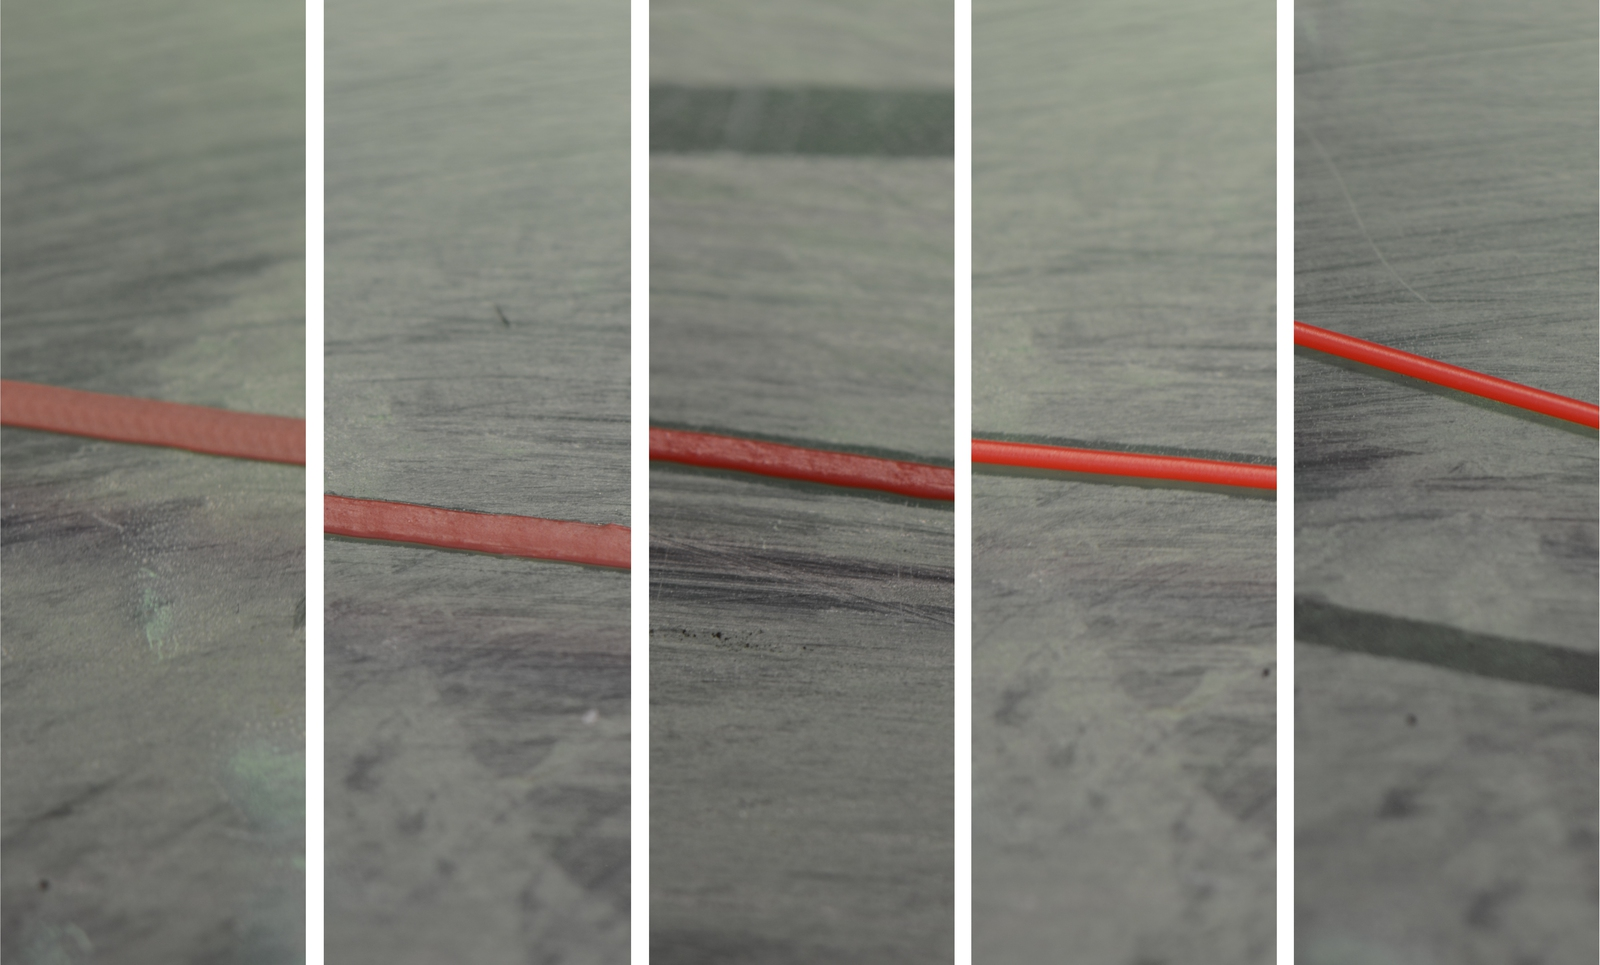
\includegraphics[keepaspectratio=true,angle=0,height=0.4\textheight,width=1.0\textwidth]{1st_layer_adhesion.jpg}
\caption{First layer adhesion}
\label{fig:1st_layer_adhesion}
\end{figure}
as an example of a good first layer adhesion. From left to right: very low, low, \emph{perfect}, high, very high. If the first layer is too high or low you can pause the print by pressing the \texttt{Pause} button. Adjust the Z end stop trigger. After making adjustments remove any printed material off the bed and home the axes and press \texttt{Restart} to restart the print. Measure the extrusion width, ideally the width would be the same in all areas of the bed. You would raise/lower a corner to minimize/increase the extrusion width to match the others. Once they are all consistent, the bed is level.

\section{Your First Octopus!}
Load the \texttt{octopus.gcode} file. This file can be found at:
\texttt{http://download.lulzbot.com/TAZ/novelties/}. Load the file in Pronterface, bring the hot end \texttt{(230C ABS/185C PLA))} and the heated bed \texttt{(85C ABS/60C PLA)} up to printing temperature. Once the printer is at the appropriate temperature, press the \texttt{Print} button to begin the print.

\section{Remove Part}
After the part is finished printing, the heated bed will automatically cool down to \texttt{60°C}. If you are printing PLA you will need to turn the heated bed off. Once the bed cools you can you pop the finished part off of the printed surface. To remove the printed part, use the clam knife included in your printer kit. Leather gloves are suggested to protect your hands from the clam knife blade. It is also safe practice to not place your hand behind the direction you are pushing the clam knife. Using the side of the clam knife blade pry up one side of the printed part. If your part is large you may need to pry at multiple points to pop the part off of the print surface. When removing parts take caution to not damage the PET film. If the film is cut or ripped it will peel from the glass and need to be replaced. Make sure to reset the heated bed to the correct temperature and allow it to heat up to the needed temperature before starting the next print.

}
\fi
%%% END FIRSTPRINT %%%

%%% MAINTENANCE %%%
\ifmaintenance
\chapter{\emph{Maintaining Your 3D Printer}}
\thispagestyle{empty}
\markboth{Maintaining Your 3D Printer}{LulzBot\textsuperscript{\miniscule{\texttrademark}} TAZ User Manual}
{\section{Overview}
\index{maintenance}
There is little maintenance needed in keeping your TAZ 3D printer running. Depending on your rate of use you will want to perform a quick check of your printer every 2-4 weeks. The following maintenance guide lines will keep your printer printing quality parts.

\section{Smooth Rods}
\index{smooth rods}
\index{bushings}
\index{lubricant}
Wipe the smooth steel rods with a clean rag or paper towel. The linear bushings leave a solid lubricant that builds up over time. If you begin hearing squeaking noises while the printer is printing, this is likely a sign that the smooth rods need to be cleaned. NOTE: never apply any lubricant or cleaning agent to the smooth rods; the bushings are self lubricating.

\section{Threaded Rods}
\index{threaded rods}
\index{grease}
Periodically, you will want to wipe down the threaded rods with silicone based grease. Never use any petroleum based grease, as it may compromise the plastic parts. Apply the silicone grease both above and below the X ends on the threaded rods and wipe down the threaded rods. Use pronterface to drive the Z axis up and down to help further distribute the lubricant.

\section{PET Sheets}
\index{PET sheet}
\index{glass}
\index{acetone}
After repeated use, the PET sheet print surface will begin to wear. Replacement PET sheets are available on \texttt{LulzBot.com}. To replace the PET print surface, peel off the worn PET sheet from the glass print surface. If there is any glue or plastic residue left on the glass surface, clean it with acetone or an alcohol based glass cleaner. Peel a corner of the clear plastic away from the green PET sheet and apply the corner of the PET to the corner of the glass. Align the PET sheet onto the glass. Using a paper towel begin slowly smoothing/applying the PET onto the glass while pulling back the clear sheet from underneath the PET. You can also spray glass cleaner onto the paper towel or the top side of the PET for a smoother application. After applying the PET sheet to the glass any bubbles can be pushed out or smoothed down using a credit card or stiff and dull piece of plastic.

\section{Hobbed Bolt}
\index{hobbed bolt}
\index{extruder jam}
The plastic filament is pulled through the extruder by a hobbed bolt. After repeated use, the teeth of the hobbed bolt can become filled with plastic. Using the brush or pick from the printer kit, clean out the hobbed bolt teeth. If an extruder jam ever occurs, remove the plastic filament from the extruder and clean out the hobbed bolt.

\section{Software}
\index{software}
\index{download}
Every quarter LulzBot will release a new stable version of the software. It is best to update the software every time a new version is released. The software is as important in printing quality parts as the hardware. Each quarterly software update can bring advances in print quality. The files are available at \texttt{http://download.lulzbot.com/TAZ/} . You can also find updated software versions in the Support/Downloads section of LulzBot.com.

\section{Belts}
\index{belts}
Over long periods or after extensive relocating of the printer you may need to re-tighten the belts on the TAZ 3D printer. For the X axis, using the 2.5mm hex driver, loosen one of the belt clamps. The belts clamps are located on the X axis carriage. To loosen the belt clamp, loosen the M3 screws on each side of the clamp. Using the needle nose pliers, pull the belt tight. While holding the belt tight, tighten down both M3 screws. The Y axis belt can be tightened in the same steps as the X axis with the belt clamps found on the bottom of the Y axis plate. Make sure not to over tighten the belts as this can cause unneeded stress on the printer.

\section{Hot End}
\index{hot end}
\index{acetone}
The hot end should be kept clean of extruded plastic by removing melted plastic strands with the tweezers. If melted plastic builds up on the hot end nozzle it can be cleaned with a paper towel soaked with acetone. Make sure the hot end is completely cool before attempting to clean the nozzle with acetone.


\section{Electronics}
\index{RAMBo}
\glossary{RAMBo}{[R]epRap [A)]duino-[M]ega compatible [M]other [Bo]ard. Designed by Joynnyr of Ultimachine.}
\index{electronics}
\index{fan}
The electronics case holding the RAMBo board may need to have dust blown out occasionally. Power down the printer and use the provided 2.5MM driver to remove the 4 M3 screws holding the lid to the enclosure. \textcolor{red}{The fan is mounted to the lid and connected to the RAMBo board. Be careful with the fan cable during removal}. Once removed use short bursts of compressed air to blow out any dust or debris. Plug in the lid fan paying attention to polarity and reattach the lid.
}
\fi
%%% END MAINTENANCE %%%

%%% ADVANCED %%%
\ifmaintenance
\chapter{\emph{Advanced Usage}}
\thispagestyle{empty}
\markboth{Advanced Usage}{LulzBot\textsuperscript{\miniscule{\texttrademark}} TAZ User Manual}
{%
% Advanced.tex
% Advanced Techniques
%
% LulzBot TAZ User Manual
%
% Copyright (C) 2015 Aleph Objects, Inc.
%
% This document is licensed under the Creative Commons Attribution 4.0
% International Public License (CC BY-SA 4.0) by Aleph Objects, Inc.
%
%

\section{Intro}
\index{advanced techniques}
\glossary{3D Printer}{Also referred to as additive manufacturing, is the process of fabricating objects from 3D model data, through the deposition of a material in accumulative layers.}
\glossary{Spool}{Plastic filament coiled and stored on a plastic reel. Preferred over 1.75-mm filament due to improved feeding and better mounting options.}
\glossary{Filament}{Plastic material in a "string" like form, as it is fed to the printer.}
\glossary{ABS}{Acrylonitrile butadiene styrene thermoplastic. Usually extrudes at 230C.}
\glossary{PLA}{Polylactic acid is a corn-based biodegradable polymer. Usually extrudes at 185C.}
\glossary{HDPE}{High-density polyethylene.}
\glossary{Polycarbonate}{A strong and impact-resistant thermoplastic. Usually extrudes at ~300C.}
\glossary{HIPS}{High-impact polystyrene.}
\glossary{Laywoo-D3}{Wooden filament similar to PLA. Forty percent of its content consists of recycled wood. Usually prints at ~180C to 210C. Color can be changed by varying the extrusion temperature.}
After you become familiar with printing using the default settings, a few advanced techniques may help in getting better and more consistent prints from the TAZ 3D printer. Some of these instructions are items and materials not included with the TAZ. With any of these additional items or materials, follow safety and usage guidelines as instructed by the manufacturer.

\section{Changing nozzles}
\index{nozzle}
\glossary{Nozzle}{The metal tip at the bottom of the hot end. It has a small hole where the plastic filament comes out of the printer.}
\index{high resolution}
%The TAZ 3D printer ships with a standard 0.35mm nozzle which allows small-layer resolution and up to 0.35mm layers. Although the 0.35mm nozzle will be perfect for most printing applications, LulzBot may also offer smaller or larger nozzle sizes in the future.
The TAZ 3D printer is available with a tool head equipped with either a 0.50mm or 0.35mm nozzle. The tool head with the 0.50mm nozzle diameter will print faster than the 0.35mm nozzle tool head. Due to the specific torque- 30 ft/lb- required to tighten the nozzle when removed we do not recommend removing the nozzle from the LulzBot Hexagon Hot End. Failure to properly tighten the nozzle to the specific recommended torque may lead to leaks or damage if over-tightened. Nozzle related issues may not be covered under warranty after nozzle changes. We recommend having the other nozzle diameter tool head/hot end on hand for quick, easy, and simple changes.
\glossary{Layer height}{The thickness of each individual deposited layer of the three-dimensional model when cut with a slicing program.}


\index{hot end}
\glossary{Hot end}{The hot end is the whole part where the plastic melts, including the nozzle, heater block, thermistor, and heat sink. The LulzBot\textsuperscript{\miniscule{\texttrademark}} Hexagon all-metal hot end comes standard on the TAZ 5.}
\index{threaded extension}
\glossary{Threaded extension}{Used to separate the heater block and nozzle from the PEEK insulator. The plastic filament passes through the threaded extension into the melting chamber.}
%\glossary{PEEK}{Polyether ether ketone: an organic polymer used to insulate the hot end due to its mechanical properties at elevated temperatures.}
%In most cases the nozzle is best changed when the hot end is slightly warm. NEVER try to remove the nozzle when the hot end is at extrusion temperature. At higher temperatures the threaded extension expands in the nozzle causing the nozzle to bind if turned. Heat the hot end to \texttt{160°C}. This will soften the plastic inside the hot end and allow the nozzle to be loosened off the threaded extension. Power off the printer and before it cools unscrew the nozzle. Take care when removing the nozzle while the hot end is hot. Wear leather gloves or use a towel to turn the nozzle off the hot end.

\index{wrench}
\index{heater block}
\glossary{Heater block}{Machined from aluminum, the heater block generates heat with a heater resistor and uses a thermistor to measure the temperature.}
\glossary{Thermistor}{A special type of resistor that changes resistance based on temperature. It is used to measure temperature on the nozzle and the heated bed.}
\glossary{Heater resistor}{A special type of resistor that is used to apply heat in a small area.}
%The LulzBot Hexagon does not currently have additional nozzle sizes. If a nozzle change is required you will need to tighten the nozzle to the recommended 30in/lb of torque. 

Prior to any modifications make sure the that printer is unplugged from both the wall and the computer. Use a 7mm wrench to turn the nozzle and a 18mm wrench to hold the heater block. A guide on assembling the LulzBot Hexagon hot end is available at \texttt{http://ohai-kit.alephobjects.com}

%\index{anti-seize}
%If you will be changing nozzles frequently we suggest reapplying a small amount of high temperature anti-seize compound to the inside threads of the nozzles. You will need an anti-seize capable of temperatures of at least \texttt{250°C}.

\section{ABS/Acetone Glue}
\label{sec:ABS/Acetone Glue}
\index{acetone}
\index{ABS}
\glossary{Acetone}{A colorless, volatile, flammable liquid ketone, (CH3)2CO, used as a solvent for ABS.}
Acetone is not included or required with the TAZ 3D printer. \textcolor{red}{Acetone and ABS solution is NOT recommended anymore, as the PEI print surface works well without it.}

\index{warping}
\index{bottle}
You may find that during printing, printed parts lift off the print surface on the corners. If you are seeing this turning on \texttt{Brim} in Cura or Slic3r will help increase the surface area of the print, improving part adhesion. If the corners of the part still lift, clean the PEI surface with IPA/ Isopropyl Alcohol and sand the surface with fine grit (2000-3000) sandpaper.

%\index{PET sheet}
%\glossary{PET}{Polyethylene terephthalate.}
%To apply the acetone/ABS mixture, put a small amount onto a paper towel. Now, rub the towel onto the cool PET print surface to apply a \emph{thin} layer of ABS. Generally only one thin layer of the acetone/ABS solution is needed. However, you can apply multiple coats if needed.

\section{Using 1.75mm filament}
\index{1.75mm filament}
\index{PTFE tube}
\glossary{PTFE}{Polytetrafluoroethylene is a synthetic fluoropolymer used in the Budaschnozzle for it's low coefficient of friction. The TAZ 5 does not use a hot end with a PTFE insert.}

Your TAZ 3D printer is set up to use 3mm plastic filament by default and may be capable of printing 1.75mm filament- your results may vary. More information can be found in our User Forums at: \texttt{https://forum.lulzbot.com/viewtopic.php?f=16\&t=1923}
}
\fi
%%% END ADVANCED %%%

%%% FAQ %%%
\iffaq
\chapter{\emph{FAQ}}
\thispagestyle{empty}
\markboth{FAQ}{LulzBot\textsuperscript{\miniscule{\texttrademark}} TAZ User Manual}
{%
% FAQ.tex
% Frequently Asked Questions
%
% LulzBot TAZ User Manual
%
% Copyright (C) 2015 Aleph Objects, Inc.
%
% This document is licensed under the Creative Commons Attribution 4.0
% International Public License (CC BY-SA 4.0) by Aleph Objects, Inc.
%

\section{Frequently Asked Questions (FAQ)}
\index{FAQ}
\begin{enumerate}
\item Our FAQ is available online in our Support Section at \texttt{https://www.lulzbot.com/support/faq}.
\end{enumerate}
}
\fi
%%% END FAQ %%%

%%% TROUBLESHOOTING %%%
\iftroubleshooting
\chapter{\emph{Troubleshooting}}
\thispagestyle{empty}
\markboth{Troubleshooting}{LulzBot\textsuperscript{\miniscule{\texttrademark}} TAZ User Manual}
{%!TEX root = Slic3r-Manual.tex

%!TEX root = Slic3r-Manual.tex

\subsection{Dimension Errors}
\label{sec:dimension_errors}
\index{Dimension Errors}

Your TAZ 3D printer has been calibrated and tested prior to leaving our Colorado factory: the steps/mm values for X, Y, and Z axes have been calculated according to your belts, pulleys and leadscrews. Please don't calibrate by trial-and-error: those values should be exact. Use our standard, known-good values already present in the firmware.

\subsubsection{Vertical dimensions}

If your vertical dimensions are wrong (i.e. along the Z axis) -and your object is usually shorter than expected- it means your nozzle is too low, thus the first layer is pressed too much on the print bed. To fix this, you might want to raise your Z endstop or increase the Z offset option in Slic3r.

If you encounter vertical dimensions that are half the expected height, make sure that you are using the appropriate firmware for your 3D printer. Instructions on firmware flashing can be found at: \texttt{https://www.LulzBot.com/Cura}.

\subsubsection{Horizontal dimensions}

The usual issue is about holes being too small. This usually only affects holes on the horizontal plane (XY). There are several reasons for this. Let's see them one by one:

\subsubsection{Plastic shrinkage}

Plastic \texttt{shrinks when cooling}. Different kinds of plastic exhibit different shrinkage rates, which might also depend on temperature. Because of such shrinkage, circular (or polygonal) holes laid by the extruder at the nominal diameter will end up smaller after cooling.

\subsubsection{More material is deposited in the inside}

When you extrude along a curve, more material per distance unit is deposited in the concave side. Such excessive material makes the internal radius shorter. A compensation algorithm\footnote{\texttt{http://reprap.org/wiki/ArcCompensation}} was proposed by Adrian Bowyer, and it was implemented in Slic3r some time ago but many users complained about holes being too large – it was removed thereafter since smaller holes are better than larger holes since they can be drilled.

\subsubsection{Curves are approximated by polygons}

STL files only contain meshes composed by flat triangles, so its planar sections can only contain polygonal shapes. For example, a circular hole is approximated by a polygon:

\begin{figure}[H]
\centering
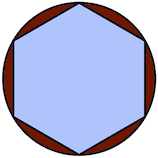
\includegraphics[keepaspectratio=true,width=0.33\textwidth]{troubleshooting/polygonal-hole.png}
\caption{Holes made through polygonal segments.}
\label{fig:polygonal-hole}
\end{figure}

Increasing the number of segments in your CAD before exporting the STL file will help reducing the error. OpenSCAD users might want to use the \texttt{polyhole()} function developed by nophead\footnote{\texttt{http://hydraraptor.blogspot.it/2011/02/polyholes.html}} that calculates the optimal number of segments.

\subsubsection{Filament tends to cut corners}

Since curves are approximated by polygons, there are sharp vertices at their vertices. However, plastic tends to make rounded corners, thus reducing the internal area of the hole even more.

\subsubsection{Z wobble}

Even if the dimensional accuracy of a single layer was correct, several stacked layers might make the hole smaller if they're not exactly aligned. Z wobble caused by mechanical issues will reduce hole size to the internal envelope of the stacked layers:

\begin{figure}[H]
\centering
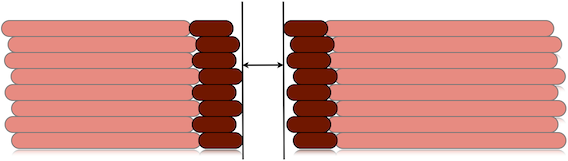
\includegraphics[keepaspectratio=true,width=1\textwidth]{troubleshooting/z-wobble.png}
\caption{Z wobble changing layer stacking.}
\label{fig:z-wobble}
\end{figure}

\subsubsection{Non-regular filament section}

Low-quality and medium-quality filaments are not very regular in diameter. If you measure their diameter along a single meter of them, you'll often find many different values (and many low-quality filaments are even not perfectly round in section). This continuous variation in diameter will produce irregular flow and the resulting hole will still be the internal envelope of all the layers:

\begin{figure}[H]
\centering
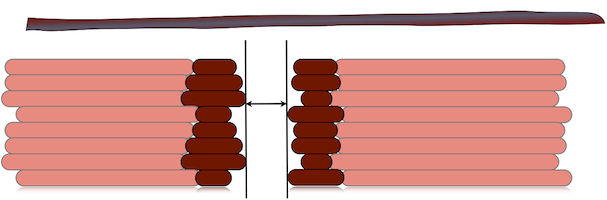
\includegraphics[keepaspectratio=true,width=1\textwidth]{troubleshooting/irregular-filament.png}
\caption{Variable filament diameter changing layer stacking.}
\label{fig:irregular-filament}
\end{figure}

\subsubsection{Backlash}

Backlash is a mechanical defect of one or more axes that basically reduces the amount of actual motion whenever a motor inverts its spinning direction. It's generally caused by loose belts. On printers with a moving bed, its axis (usually Y) is more subject to backlash because of inertia. So, if you get different dimension errors in X and Y, that's caused by backlash. You'll need to tighten your belts.

\subsubsection{Flow Math}
The above causes do not depend on Slic3r and, when possible, they need to be fixed before attempting any software solution.

That said, the flow math used in Slic3r plays a good role in making correct dimensions, since it tries to guess what the shape of the extruded material will be and how thick the extrusion will result on the horizontal plane given an amount of material. Being an approximation, it carries an error. The usual way to deal with these issues involves tuning the Extrusion Multiplier setting in order to increase/reduce the amount of plastic, thus making extrusions more or less thick. But this will also affect solid surfaces, so it's not the ideal solution.

For more exact dimensions you need to check the External Perimeters First option. Printing external perimeters first will prevent the shift caused by extrudate overlap. On the other hand, printing internal perimeters first hides seams better, so it's your take.

A new XY Size Compensation option was also introduced that allows to grow/shrink object shapes in order to compensate for the measured error. Supposing your holes are smaller by 0.1mm, you can just enter -0.05 in this option to get them compensated (negative sign means shrink inwards). This is not recommended.



%!TEX root = Slic3r-Manual.tex

\subsection{Z Wobble} % (fold)
\label{sec:z_wobble}
\index{Z Wobble}


Undulations in the walls of a print may be due to wobble in the Z axis.  A thorough analysis of the potential causes is given by whosawhatsis\footnote{\	exttt{http://goo.gl/iOYoK}} in his article "Taxonomy of Z axis artifacts in extrusion-based 3d printing"\footnote{http://goo.gl/ci9Gz}, however one point of particular interest for users of Slic3r is the wobble caused by motor steps not matching the pitch of the Z rods thread.  This can be addressed by ensuring the \texttt{Layer Height} setting is a multiple of the full step length.


The relevant part of the above paper is quoted here:

\quote{To avoid Z ribbing, you should always choose a layer height that is a multiple of your full-step length. To calculate the full-step length for the screws you're using, take the pitch of your screws (I recommend M6, with a pitch of 1mm) and divide by the number of full-steps per rotation on your motors (usually 200). Microsteps are not reliably accurate enough, so ignore them for this calculation (though using microstepping will still make them smoother and quieter). For my recommended M6 screws, this comes out to 5 microns. It's 4 microns for the M5 screws used by the i3, and 6.25 microns for the M8 screws used by most other repraps. A layer height of 200 microns (.2mm), for example, will work with any of these because 200 = 6.25 * 32 = 5 * 40 = 4 * 50.}


% subsection z_wobble (end)


\newpage

}
\fi
%%% END TROUBLESHOOTING %%%

%%% SOURCE %%%
\ifsource
\chapter{\emph{Hardware and Software Source Code}}
\thispagestyle{empty}
\markboth{Hardware and Software Source Code}{LulzBot\textsuperscript{\miniscule{\texttrademark}} TAZ User Manual}
{%
% Source.tex
% Where to get source code for the printer and manual.
%
% LulzBot TAZ User Manual
%
% Copyright (C) 2014 Aleph Objects, Inc.
%
% This document is licensed under the Creative Commons Attribution 4.0
% International Public License (CC BY-SA 4.0) by Aleph Objects, Inc.
%

\index{source code}
\index{download}
The LulzBot\textsuperscript{\miniscule{\texttrademark}} TAZ 3D printer is a free/libre hardware design. All of the source files are available at \texttt{http://download.lulzbot.com/TAZ} including:

\begin{itemize}
\index{latex}
\item The latest version of this document, with {\LaTeX} source code.

\index{STL}
\index{gcode}
\index{printed parts}
\item 3D models and print files for all of the printed parts in \texttt{.stl}, \texttt{.gcode}, and other original source files.

\index{calibration}
\index{novelties}
\item 3D calibration objects and random novelties.

\item Production file for calculating large print runs.

\index{electronics}
\item Design files for all electronics and machined parts.

\begin{itemize} % 2nd level
\index{Budaschnozzle}
\item Budaschnozzle hot end
\index{RAMBo}
\item RAMBo electronics
\item Various spec sheets
\end{itemize} % end 2nd level

\index{bill of materials}
\item Bill of materials including every part needed to build the printer.
\begin{itemize} % 2nd level
\item TAZ
\index{Budaschnozzle}
\item Budaschnozzle
\end{itemize} % end 2nd level

\index{hardware}
\item Drawings of components.
\begin{itemize} % 2nd level
\index{aluminum extrusions}
\item Aluminum extrusions
\item Budaschnozzle
\index{bed plate}
\item Bed plate
\end{itemize} % end 2nd level

\index{software}
\item Software binaries and source code for GNU/Linux and others. Also includes known good configuration files.
\begin{itemize} % 2nd level
\index{Slic3r}
\item Slic3r
\index{Printrun}
\item Printrun
\index{Marlin}
\item Marlin
\end{itemize} % end 2nd level

\end{itemize}

}
\fi
%%% END SOURCE %%%

%%% SUPPORT %%%
\ifsupport
\chapter{\emph{3D Printer Support}}
\thispagestyle{empty}
\markboth{3D Printer Support}{LulzBot\textsuperscript{\miniscule{\texttrademark}} TAZ User Manual}
{%
% Support.tex
% How to get technical support.
%
% LulzBot TAZ User Manual
%
% Copyright (C) 2014 Aleph Objects, Inc.
%
% This document is licensed under the Creative Commons Attribution 4.0
% International Public License (CC BY-SA 4.0) by Aleph Objects, Inc.
%

\section{LulzBot}
\index{technical support}
\setlength{\parindent}{0pt}
For common technical support questions for your TAZ 3D printer please visit \texttt{lulzbot.com/support}. Also, visit \texttt{forum.lulzbot.com} for support and tips from the LulzBot community. If you have further questions, e-mail our support team at \texttt{support@lulzbot.com}. Please completely read this manual before contacting for support questions or help. The latest version of this information guide is also available at \texttt{http://download.lulzbot.com}. You can also find more information including images, videos, and updated versions of this manual in the Support section of LulzBot.com.

\section{Community}
\index{community support}
\index{Freenode}
\index{IRC}
\index{RepRap}
\index{forums}
Community Support and Resources

\begin{itemize}

\item LulzBot forum: \texttt{forum.lulzbot.com}
\item IRC chat rooms on the \texttt{irc.freenode.net} server.
	\begin{itemize}
	\item \texttt{\#reprap}: Highly active community chat room where help can easily be found
	\item \texttt{\#slic3r}: Slic3r chat room where Slic3r developers and users can give help
	\end{itemize}
\item RepRap.org forums: \texttt{forums.reprap.org}

\end{itemize}
}
\fi
%%% END SUPPORT %%%

%%% CONTACT %%%
\ifcontact
\chapter{\emph{Contact Information}}
\thispagestyle{empty}
\markboth{Contact Information}{LulzBot\textsuperscript{\miniscule{\texttrademark}} TAZ User Manual}
{%
% Contact.tex
%
% LulzBot TAZ User Manual
%
% Copyright (C) 2014 Aleph Objects, Inc.
%
% This document is licensed under the Creative Commons Attribution 4.0
% International Public License (CC BY-SA 4.0) by Aleph Objects, Inc.
%

\section{Support}
\setlength{\parindent}{0pt}
Email: \texttt{support@LulzBot.com}

Phone: +1-970-377-1111 x610

\section{Sales}

Email: \texttt{sales@LulzBot.com}

Phone: +1-970-377-1111 x600

\section{Websites}

Aleph Objects, Inc., the makers of LulzBot 3D Printers:

\texttt{www.AlephObjects.com}


LulzBot 3D Printers and parts:

\texttt{www.LulzBot.com}

\texttt{forum.LulzBot.com}
}
\fi
%%% END CONTACT %%%

%%% END MAINMATTER %%%
%%% BEGIN BACKMATTER %%%
\backmatter

%%% INDEX %%%
\clearpage
\printindex
%%% END INDEX %%%

%%% GLOSSARY %%%
\renewcommand{\memgloterm}[1]{\textbf{#1}}
\renewcommand{\memglodesc}[1]{\textit{#1}}
\renewcommand{\memglonum}[1]{}

\clearpage
\printglossary
%%% END GLOSSARY %%%

%%% COLOPHON %%%
\ifcolophon
%%% skip a couple pages
\pagebreak{}
\thispagestyle{empty}
\begingroup 
\vfill\null 
\endgroup
\pagebreak{}
\thispagestyle{empty}
{%
% Colophon.tex
%
% LulzBot TAZ User Manual
%
% Copyright (C) 2014 Aleph Objects, Inc.
%
% This document is licensed under the Creative Commons Attribution 4.0
% International Public License (CC BY-SA 4.0) by Aleph Objects, Inc.
%

%%% COLOPHON %%%
\begin{vplace}
\centering
\emph{\LARGE Colophon}

\rule{0.5\textwidth}{0.4pt}\\[\baselineskip]

{\tiny Created with 100\% Free/Libre Software}

GNU/Linux

{\LaTeX} Memoir

% XXX surely a less dumb way to make some space :)
\rule{0\textwidth}{0pt}\\[\baselineskip]%
\rule{0.5\textwidth}{0.4pt}\\[\baselineskip]
\end{vplace}
%%% END COLOPHON %%%
}
\fi
%%% END COLOPHON %%%
%%% END BACKMATTER %%%

%%% BLANK PAGES Lulu requires minimum 68 pages %%%
\thispagestyle{empty}
\begingroup
\newpage
\mbox{}
\thispagestyle{empty}
\newpage
\mbox{}
\thispagestyle{empty}
\newpage
\mbox{}
\thispagestyle{empty}
\newpage
\mbox{}
\thispagestyle{empty}
\newpage
\mbox{}
\thispagestyle{empty}
\newpage
\endgroup
%%% END BLANK PAGE %%%

\end{document}

